%%%%%%%%%%%%%%%%
% Ph.D. thesis %
%%%%%%%%%%%%%%%%

%\documentclass[12pt,openright,twoside,letterpaper,onecolumn]{report} %% USE THIS FOR DOUBLE SIDED
\documentclass[12pt,openright,oneside,letterpaper,onecolumn]{report}  %% USE THIS FOR SINGLE SIDED

\includeonly{
	header,
	ack,
	intro,
	janus/janus,
	aspherical,
	2dsoft/2dsoft,
	brush/brush,
	pixel/pixel,
	conclusions
}

\newcommand{\comment}[1]{}

\newcommand{\thesistitle}{Self-organization in systems of anisotropic particles}
\newcommand{\thesisauthor}{William Leneal Miller III}
\newcommand{\thesisyear}{2012}

%%%
%%% Packages
%%%
%\usepackage[dvips]{epsfig}
\usepackage{amsmath}
\usepackage{amssymb}
\usepackage{named}
\usepackage{fancyhdr}
\usepackage{afterpage}
%\usepackage{subfigure}
\usepackage[config=altsf.cfg]{subfig}
\usepackage{graphicx}
\usepackage{color}
\usepackage[sort&compress,numbers]{natbib}
\usepackage{dcolumn}
\usepackage{multirow}
\usepackage{array}
%\usepackage{doi}
\usepackage[T1]{fontenc}

%
% We use the hyperref package and customize it for optimal PDF 
%
%\usepackage[dvipdfm,pdftitle={\thesistitle},pdfauthor={\thesisauthor},pdfpagemode={UseOutlines},letterpaper,bookmarks,bookmarksopen=true,pdfstartview={FitH},bookmarksnumbered=true,]{hyperref}
%\usepackage[pdftex,pdftitle={\thesistitle},pdfauthor={\thesisauthor},pdfpagemode={UseOutlines},letterpaper,bookmarks,bookmarksopen=true,pdfstartview={FitH},bookmarksnumbered=true,colorlinks,linkcolor=blue,citecolor=blue,urlcolor=blue,linktocpage]{hyperref}
\usepackage[pdftex,pdftitle={\thesistitle},pdfauthor={\thesisauthor},pdfpagemode={UseOutlines},letterpaper,bookmarks,bookmarksopen=true,pdfstartview={FitH},bookmarksnumbered=true,colorlinks,linkcolor=black,citecolor=black,urlcolor=black,linktocpage]{hyperref}

%%%
%%% Margins
%%%
\paperwidth=8.5in
\paperheight=11in

% 1in + hoffset + oddsidemargin + textwidth + marginparsep + marginparwidth
% For PhD at Columbia we have single side theses and 1.5in left margin
% The settings below leave 1.5 inch margin at the left and 1 inch at the right 
% for US Letter paper
\setlength{\hoffset}{0.0in}
\setlength{\oddsidemargin}{.25in}
\setlength{\textwidth}{6in}
\setlength{\evensidemargin}{.25in}

% 1in + voffset + topmargin + headheight + headsep + textheight + footskip 
% For PhD thesis we also need an extra inch at the bottom
% 1inch = 72 pt
\setlength{\voffset}{0.0in}
\setlength{\topmargin}{.0in}
\setlength{\headheight}{14pt}
\setlength{\headsep}{22pt}
\setlength{\textheight}{8.5in}
\setlength{\footskip}{0pt}

\newcommand{\inbox}[1]{\multicolumn{1}{|>{\centering}m{0.12\textwidth}|}{#1}}
\newcommand{\edit}[1]{#1}

%%%
%%% Spacing
%%%
\newcommand{\singlespace}{\renewcommand{\baselinestretch}{1.15} \small \normalsize}
\newcommand{\oneandhalfspace}{\renewcommand{\baselinestretch}{1.3} \small \normalsize}
\newcommand{\doublespace}{\renewcommand{\baselinestretch}{1.5} \small \normalsize}
\newcommand{\normalspace}{\doublespace}
\footnotesep=1\baselineskip

%%%
%%% Counters depth
%%%
\setcounter{secnumdepth}{3}
\setcounter{tocdepth}{3}

%%%
%%% Title page.
%%%
\newcommand{\thesistitlepage}{
    \singlespace
    \thispagestyle{empty}
    \begin{center}
        {\large\textcolor{white}{.}\\[4cm]
		\textbf{\thesistitle} \\[1cm]
        \thesisauthor \\[6cm]
        %\textbf{\LARGE \thesistitle} \\[1cm]
        %\textbf{\LARGE \thesisauthor} \\[8cm]
        Submitted in partial fulfillment of the \\
        requirements for the degree \\
        of Doctor of Philosophy \\
		under the Executive Committee \\
        of the Graduate School of Arts and Sciences \\[2cm]
        COLUMBIA UNIVERSITY \\[5mm]
        %\textbf{\Large COLUMBIA UNIVERSITY} \\[5mm]
        \thesisyear}
    \end{center}
    \clearpage
	\normalspace
}
%%%
%%% Copyright page.
%%%
\newcommand{\thesiscopyrightpage}{
    \thispagestyle{empty}
    \strut \vfill
    \begin{center}
      \copyright \thesisyear \\
      \thesisauthor \\
      All Rights Reserved
    \end{center}
    \cleardoublepage
}

%%%
%%% Abstract page.
%%%
\newcommand{\thesisabstract}{
    \thispagestyle{empty}
    \begin{center}
    \textbf{ABSTRACT} \\[5mm]
     \textbf{\thesistitle} \\[5mm]
     \textbf{\thesisauthor} \\[1cm]
    \end{center}
    This dissertation presents studies on self-organization in soft matter systems.
A wide variety of systems is studied, with the goal of understanding both the nonequilibrium and the equilibrium properties of this important process.

In Chapter~\ref{chap:janus}, we study the self-assembly of asymmetric Janus colloidal particles.
We identify and systematically describe the effect of the ratio of hydrophobic to hydrophilic surface area on the nonequilibrium processes and structure formation.

In Chapter~\ref{chap:aspherical}, we examine systems of hard, aspherical particles.
We demonstrate that the thermodynamics of self-organization of a system of these aspherical particle (either a system of identical particles or a polydisperse system of different-shaped particles) is well-predicted by a simple relationship between the crystallization pressure and two measures of particle asphericity borrowed from other fields.

In Chapter~\ref{chap:2dsoft}, we shift focus to systems of soft particles in two dimensions and on the surface of a sphere.
Soft particles are particles with a finite interaction potential at zero distance; such particles exhibit a surprisingly large variety of ordered structures at equilibrium.
A similar phenomenon is seen when the study is extended to soft particles on the surface of a sphere.

In Chapter~\ref{chap:brush}, we study the free energy of two-component polymer brush systems in which polymers of different length are patterned in alternating stripes of specified widths on the surface of a cylinder.
We present the dependence of the free energy on the polymer lengths and stripe width and a qualitative explanation of its functional form.

Finally, in Chapter~\ref{chap:pixel}, we approach the reverse self-assembly problem.
That is, we describe an algorithm for answering the reverse (and much more difficult) question, ``Given a specific desired target self-assembled structure, what interparticle interactions will yield a system which will self-assemble into that structure?''
We also describe a new model of interparticle interaction which should be able to generate interparticle interaction geometries with a high degree of flexibility.



%\section*{Hierarchical self-assembly of asymmetric Janus particles}
% From dumbbells to FCC crystals, we  study the self-assembly pathway
% of amphiphatic, spherical colloidal particles as a function of the size of the hydrophobic region using  molecular dynamics simulations.  Specifically, we analyze
% how local inter-particle interactions correlate to the final self-assembled aggregate and how they affect the dynamical pathway of structure formation.
% We present a detailed diagram separating the many phases that we find for different sizes of the hydrophobic area, and uncover a narrow region where particles self-assemble into hollow, faceted
% cages that could potentially find interesting engineering applications.
%
%\section*{Phase behavior of hard aspherical particles}
%We use numerical simulations to understand how random deviations from the ideal spherical shape affect the ability of hard particles to form
%fcc crystalline structures. Using a system of hard spheres as a reference,
%we determine the fluid-solid coexistence pressures of both shape-polydisperse and monodisperse systems of aspherical hard particles.
%We find that when particles are sufficiently isotropic,  the coexistence  pressure can be predicted from
%a linear relation involving the product of two simple geometric parameters characterizing the asphericity  of the particles.
%Finally, our results allow us to gain direct insight into the crystallizability limits of these systems by rationalizing
%empirical data obtained for analogous monodisperse systems~\cite{disorder1}.
%
%We use numerical simulations to study the crystallization of monodisperse systems of  hard aspherical particles.
%We find that particle shape and crystallizability can be easily related to each other when particles are
%characterized in terms of two simple and experimentally accessible order parameters: one based on the
%particle surface-to-volume ratio, and the other on the angular distribution of the
%perturbations away from the ideal spherical shape. We present a phase diagram obtained by exploring the
%crystallizability of  487 different particle  shapes across the two-order-parameter spectrum. Finally, we
%consider the physical properties of the crystalline structures accessible to aspherical particles, and
%discuss limits and relevance of our results.
%
%\section*{Exploiting Classical Nucleation Theory for reverse self-assembly}
%In this paper we introduce a new method to design interparticle interactions to target arbitrary crystal structures via the process of self-assembly.
%We show that it is possible   to exploit the curvature of the crystal nucleation free-energy barrier to sample and select optimal
%interparticle interactions for self-assembly into a desired structure.
%We apply this method to find interactions to target two simple crystal structures: a crystal with simple cubic symmetry
%and a two-dimensional plane with square symmetry embedded in a three-dimensional space.
%Finally, we discuss the potential and limits of our method and
%propose a general model by which a functionally infinite number of different interaction geometries may be constructed
%and to which our reverse self-assembly method could in principle be applied.
%
%\section*{Two-dimensional packing of soft particles and the soft generalized Thomson problem}
%We perform numerical simulations of \edit{a model of} purely repulsive
% soft colloidal particles interacting via a generalized elastic potential and
%constrained to a two-dimensional plane and to the surface of a spherical shell.
%For the planar case, we compute the phase diagram in terms of the system's rescaled density and temperature.
%We find that a large number of ordered phases becomes accessible at low temperatures as the density of the system
%increases, and we study systematically how structural variety depends on the functional shape
%of the pair potential.
%For the spherical case, we revisit the generalized Thomson problem for small numbers of particles $N\leq12$
%and identify, enumerate and compare the minimal energy polyhedra established by the location of the
%particles to those of the corresponding electrostatic system.
%
%\section*{Free energy of alternating two-component polymer brushes on cylindrical templates}
%We use computer simulations to investigate the stability of a two-component polymer brush de-mixing
%on a curved template into phases of different morphological properties. It has been previously shown via molecular dynamics simulations that immiscible chains having different length and anchored to a cylindrical template will phase separate into striped phases of different widths oriented perpendicularly to the cylindrical axis.
%We calculate free energy differences for a variety of stripe widths, and extract simple relationships between the sizes of the two polymers, $N_1$ and $N_2$, and the free energy dependence on the stripe width.
%We explain these relationships using simple physical arguments based upon previous theoretical work on the free energy of polymer brushes.
%

    \cleardoublepage
}

\renewcommand\bibname{References}

%%%
%%% Miscellaneous
%%%
\newcommand{\draft}{
    \renewcommand{\normalspace}{\singlespace}
    \normalspace
    \chapter*{Draft. Version \today}
\clearpage }


\begin{document}

% For the first pages we do not have numbering 
\pagestyle{empty}

\thesistitlepage
\thesiscopyrightpage

\thesisabstract

% In the "roman-numbered" section of the thesis, we have numbers at the bottom
% and we have to reduce the textheight of the text to make space for the number

\pagenumbering{roman}
\pagestyle{plain}

\setlength{\footskip}{0.5in}

\setcounter{tocdepth}{2}
\renewcommand{\contentsname}{Table of Contents}
\tableofcontents
\cleardoublepage

\listoffigures
\cleardoublepage

%\listoftables 
%\cleardoublepage

%%%
%%% Acknowledgments
%%%
~\\[1in] % hack to put space at top.
\textbf{\Huge Acknowledgments}\\

\noindent 
First, I would like to thank my advisor, Prof. Angelo Cacciuto, for giving me the honor of being his first graduate student and being a never-ending source of ideas and knowledge.
Angelo always encouraged me to work hard and tackle interesting problems with his enthusiasm and support; working with him has been a pleasure, and I honestly can't imagine a better mentor. 
I hope that this dissertation will effectively convey the exciting work we did together.

I am also grateful to my defense committee: Prof. Bruce Berne and Prof. David Reichman, who have served on my graduate committee for the past five years and provided insightful feedback on my second-year defense and original research proposal, and, along with Prof. Luis Campos and Prof. Sanat Kumar, have taken the time out of their incredibly busy schedules to read my dissertation and attend my defense.

Scientific research is a collaborative effort, and I have benefited from exceptional collaboration with other members of the Cacciuto group.
In particular, I had the privilege of working extensively with Dr. Behnaz Bozorgui Katherine Klymko, Dr. Josep P\`{a}mies, and Maya Sen.
I would also like to thank Leo PeBenito and Clarion Tung, with whom my collaboration has been less direct but no less valuable, and especially An{\dj}ela \v{S}ari\'{c} -- for large parts of the past four years, the two of us have \textit{been} the Cacciuto group. 

I would like to thank my many friends here at Columbia.
They made graduate school much more enjoyable, and I wish them all the best as they transition from school to the real world.

\newpage
I want to express my sincere gratitude to my family.
They have always been my strongest supporters, and have always been there for me unconditionally; my academic success would not have been possible without the encouragement my parents have given me since I was a child.

Finally, of course, I am thankful to Christine Vanos.
Graduate school isn't easy, but she made it much easier, and I'm looking forward to spending the rest of my life with her.

%\hspace{0.7\textwidth}{\today} \\
\hspace{0.7\textwidth}William L. Miller

\cleardoublepage

%%%
%%% Dedication page
%%%
\thispagestyle{plain}
\strut \vfill
\centerline{\Large 
\textit{For my family}
}
\vfill \strut
\cleardoublepage

%\draft   % Generates a draft version in single-space

%%%
%%% BODY
%%%
\pagestyle{headings}
\pagenumbering{arabic}

%
% In the "arabic" section of the thesis, we do not have numbers at  the
% bottom and we want to use the full length of the page to avoid vbox
% underfulls. We use the fancyheaders package to adapt the headers
% according to the  Columbia requirements.
%
\setlength{\textheight}{8.5in}
\setlength{\footskip}{0in}

% We change the pagestyle 
\fancypagestyle{plain} {%
\fancyhf{}
\fancyhead[LE,RO]{\thepage}
\fancyhead[RE,LO]{\textsl \leftmark}
\renewcommand{\headrulewidth}{0pt}
}
\pagestyle{plain}

%\chapter{Introduction}
\label{section:intro}
\chapter{Introduction}
\label{chap:intro}

\section{Soft matter physics}\label{sec:softmatt}

Broadly speaking, the results presented in this dissertation involve those physical systems in which nontrivial collective behavior emerges from the competition among hydrophobicity, entropy, and elasticity.
These systems are a subset of the broad field of soft matter physics, also referred to as complex fluids.
In general, soft matter physics revolves around materials in which their constituents have a size in the range $10$ nm -- $1$ $\mu$m, their dynamics are mostly diffusive, and thermal fluctuations play an important role -- that is, the relevant energy scales of important physical behaviors of these systems are comparable with the thermal energy at room temperature: roughly $0.6$ kcal$\cdot$mol$^{-1}$.
I will be primarily concerned with colloids and polymers; other systems such as liquids, gels, and biological materials (such as membranes) are also included in this field.

Soft materials exhibit a number of characteristics not seen in ``hard'' condensed matter.
One of the most important is the formation of mesoscopic structures, which are intermediate in scale between the individual components (e.g. colloids or polymers) and the bulk, macroscopic system.
Soft matter systems also tend to undergo large fluctuations due to their relatively low energy density, and their most interesting equilibrium properties tend to be dominated by entropy rather than energy.
The result is that soft matter systems often exhibit unique behaviors which are difficult to predict.

An example of such complicated dynamics is in the crystallization of binary systems of hard colloids; that is, systems containing hard, purely repulsive spheres of two different sizes~\cite{FrenkelNatMat}.
Because these particles cannot overlap and interact only via their hard repulsions, the energy in such systems is by definition zero.
However, a wide range of three-dimensional crystalline structures is found, depending on the relative sizes and concentrations of the two components; these interesting effects must necessarily be due solely to the configurational entropy of the system.

Over the last fifty years, a large effort has been devoted to establishing the theoretical and numerical tools with which to characterize and predict the phase behavior of complex fluids.
Most studies have focused on systems where the effective interactions between the main components are solely dependent on the interparticle separation.
However, recent advances in synthesis of nanoparticles~\cite{DeVries,Schnablegger,Hong,Weller,Hobbie,weitz,pine,mitragotri} have allowed for unprecedented control over the  shape and surface chemistry of colloidal particles;
it has also become feasible to engineer interactions between star polymers or dendrimers by controlling their overall chemical and topological properties~\cite{mladek}.
The result is an unlimited number of potential building blocks whose organization, either from a dilute fluid by aggregation due to interparticle attractions or from a dense fluid by an externally-applied pressure, have the potential to form a large variety of structures with novel functional, mechanical, and optical properties.

\section{Self-organization}

This dissertation deals with the process by which these mesoscopic and/or the full macroscopic structures form.
The work presented is the result of Monte Carlo and molecular dynamics simulations on a wide variety of systems representing a small subset of the variety described above, directed at studying the ways in which the details of interparticle interactions affect how self-organization occurs.

This self-organization of structures can be considered as divided between two broad situations: formation of macroscopic structures, which can be modeled by classical nucleation theory, and aggregation into mesoscopic structures, which is described in the framework of self-assembly theory.

\subsection{Classical nucleation theory}\label{sec:CNT}

Although the generic features of particle aggregation can be described, at least phenomenologically, in terms of simple thermodynamic arguments~\cite{Israelachvili, Zhang, Leckband, Nagarajan, glotzer2}, the details of the self-organization process are far from being understood, even in the simple case of aggregation of isotropic particles into macroscopic three-dimensional crystals.
For more complex particles, it is difficult to predict, \textit{a priori}, the equilibrium self-assembled state, and, even more interestingly, the nonequilibrium pathways associated with it.~\cite{Hong2}.

The thermodynamics of crystal formation can be described, to a first approximation, within the framework of classical nucleation theory (CNT).
In this theory, the nucleation and eventual crystallization of a system is described as a simple interplay between two competing thermodynamic forces; however,
it includes some fairly severe approximations which make it applicable only for a qualitative understanding of the process.

Consider a system of $N$ particles interacting via some potential.
Within this system is a roughly spherical nucleus of $n$ crystalline particles surrounded by a fluid of the remaining $(N-n)$ particles (note that for small $n$, the approximation of a spherical shape is a poor one).
Figure~\ref{fig:xtal} shows an illustration of this system.
There are two major contributions to the free energy of this nucleus: the free energy gain associated with the formation of the more stable crystal phase, and the free energy cost due to the interface between the fluid and the solid phase.
Below I will focus on these two terms in more detail.
\begin{figure}
	\begin{center}
		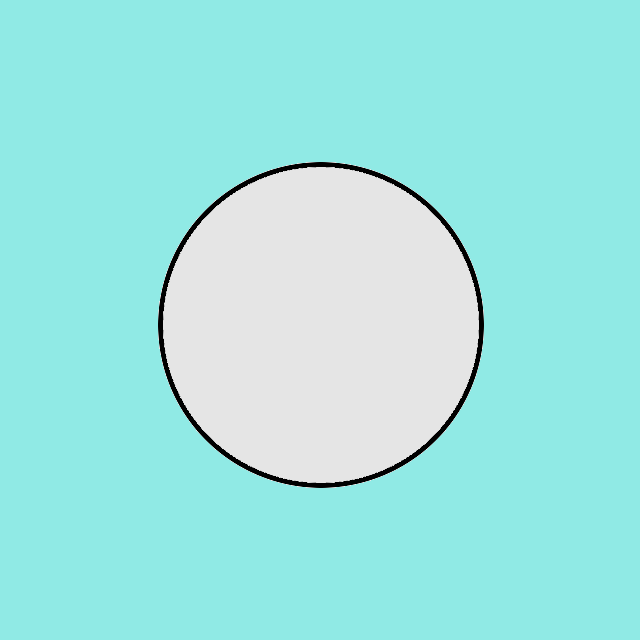
\includegraphics[width=0.4\textwidth]{xtal.png}
		\put(-117.5,80){\LARGE{Crystal}}
		\put(-110,15){\LARGE{Fluid}}
	\end{center}
	\caption[An illustration of a spherical crystal in the presence of a fluid]{An illustration of the system considered in classical nucleation theory; a spherical crystal embedded in a fluid phase.  The dark border indicates the interface.}\label{fig:xtal}
\end{figure}

%\subsection{The free energy gain due to organization}

For a typical scenario of a system of particles interacting via a short-ranged attractive potential, at sufficiently large density $\rho$, the free energy associated with the growth of the crystal is favorable because the chemical potential difference, $\Delta \mu$, between the fluid and crystalline phases becomes negative.
The condition that $\Delta \mu < 0$ is generally due to a combination of several factors; the most obvious contribution is a direct consequence of favorable interparticle energetics.
A particle in a crystal has, on average, more neighbors than one in the fluid, and thus, crystallization leads to an energy gain.
However, a favorable $\Delta \mu$ may also arise in systems featuring purely repulsive interparticle interactions, and the origin of this effect is more subtle.

For illustration, consider a system of hard spheres.
These particle interact via the potential
\begin{equation}V = \begin{cases} \infty & \textrm{if } r < r_0 \\ 0 & \textrm{otherwise}\end{cases}\,,\end{equation}
where $r$ is the distance between particles and $r_0$ is the particle diameter; therefore, as in the example system discussed in Section~\ref{sec:softmatt}, their phase bahavior is completely determined by their configurational entropy -- the interaction energy within such a system is by definition always zero.
However, very early computer simulations~\cite{Wood,Alder} showed that even these simple systems showed a transition from a fluid to a stable, face-centered cubic (fcc) crystal.

The existence of a stable crystalline phase for hard spheres implies that beyond some density $\rho$, the configurational entropy of the ordered, crystalline phase is higher than that of a disordered phase.
However, intuition and a simple consideration of the system neglecting the correlation between particles due to their excluded-volume (repulsive) interactions in the hard sphere system leads one to the conclusion that the disordered phases is higher in entropy at every density.
This indicates that excluded-volume effects must be vital for this transition, and indeed, it is clear that such effects must be important at high $\rho$.

At high enough density $\rho$, the disordered fluid phase becomes over-compressed -- the particles can no longer easily diffuse past each other and the system becomes stuck in a disordered but ``jammed'' state.
The key to understanding the existence of the crystalline state of hard spheres then is that the amount of free volume available to each particle in a fcc crystal is larger than that avilable to each particle in an over-compressed fluid.
Each particle in the crystal is therefore a bit freer to move than the particles in the disordered fluid -- and so the system has a slightly higher configurational entropy.

Thus, even in purely repulsive systems such as hard spheres, when the density $\rho$ is large enough, the free energy of crystalization, $\Delta \mu$, is negative, due to the gain in configurational entropy upon self-organization.

This negative $\Delta \mu$ results in a linear decrease of the Gibbs free energy with the number of crystalline particles in the interior of the nucleus; for large-enough spherical nuclei, it is approximately
\begin{equation}\Delta G_{\mu} (r) \simeq \frac{4}{3} \pi r^3 \rho \Delta \mu \,,\end{equation}
where $r$ is the radius of the nucleus and $\rho$ is the crystal density.
The chemical potential difference $\Delta\mu$ can easily be determined numerically; however, what is important for this qualitative understanding of classical nucleation is that in order for crystal nucleation to occur, $\Delta \mu$ must be negative.

%\subsection{Interfacial free energy}

The second major term in the full free energetic description of crystal nucleation is the free energy cost associated with the creation of an interface between the crystal nucleus and the fluid phase.
One can think of this term as arising from the loss of entropy of a particle bound to the surface versus one in the fluid, without benefit of a full complement of favorable interactions with neighbors (for attractive particles) or the full configurational entropy gain of increased free volume (for purely repulsive ones) experienced by a particle in the interior.
It is described by the surface tension $\gamma$, a quantity the value of which, like $\Delta \mu$, is unimportant for our purposes except that it must be positive.
The interfacial free energy is then the product of the surface area times the surface tension
\begin{equation}\Delta G_{\gamma} (r) = A \gamma = 4 \pi r^2 \gamma \,.\end{equation}

%\subsection{Consequences and limitations of CNT}
We thus find the total Gibbs free energy of the crystal nucleus, as a function of the nucleus size $r$,
\begin{equation}\Delta G \simeq \frac{4}{3} \pi r^3 \rho \Delta \mu + 4 \pi r^2 \gamma \,.\end{equation}
Taking the derivative of this quantity and setting the result equal to zero, a local maximum in the free energy is located at
\begin{equation}r^* \simeq \frac{2 \gamma}{\rho \left|\Delta \mu \right|} \,,\end{equation}
or, in terms of the number of particles in the cluster,
\begin{equation}n^* \simeq V_c \rho \simeq \frac{4}{3} \pi \left(r^*\right)^3 \rho \simeq \frac{32 \pi}{3 \rho}\left(\frac{\gamma}{\left|\Delta \mu\right|}\right)^3\,\,\,.\end{equation}

This is termed the ``critical nucleus size'', and represents a transition point: $50\%$ of particles of size $r^*$ would be expected to melt back to the fluid phase, and $50\%$ would be expected to grow into very large crystals.
In fact, in this approximation, nuclei larger than $r^*$ would be expected to grow until they included every particle in the system.

\begin{figure}
	\begin{center}
		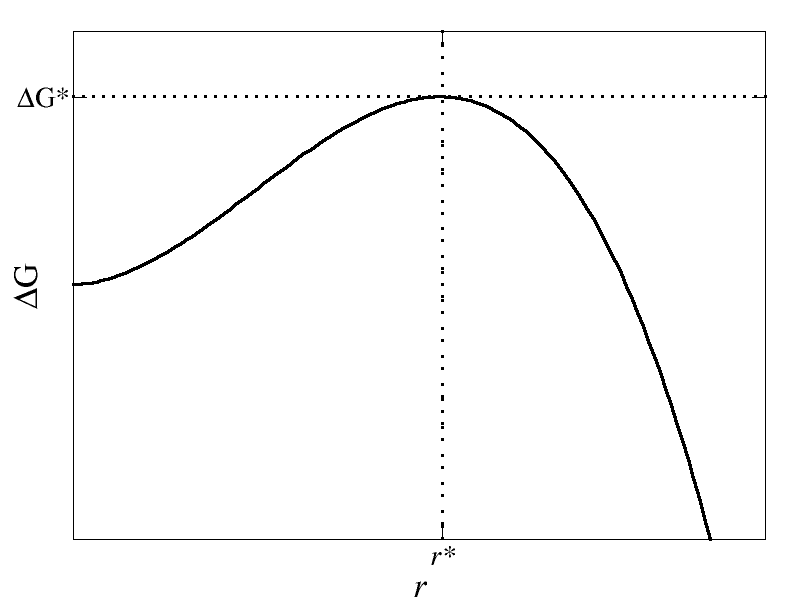
\includegraphics[width=0.6\textwidth]{CNT.png}
	\end{center}
	\caption[$\Delta G$ vs. $r$ in classical nucleation theory]{A plot of $\Delta G$ vs. $r$ for a crystal nucleus surrounded by a fluid.  The critical nucleus is at the point where the dotted lines, indicating $\Delta G^*$ and $r^*$, cross.}\label{fig:CNT}
\end{figure}

Plugging the critical radius $r^*$ into the expression for $\Delta G$ derived above yields the free energy cost of the critical nucleus,
\begin{equation}\Delta G^* \simeq \frac{16 \pi \gamma^3}{\rho^2 \Delta \mu^2}\,.\label{eq:dGCNT}\end{equation}
An illustration of the form of this free energy landscape is plotted in Figure~\ref{fig:CNT}.

In order for large, crystalline aggregates to form via classical nucleation, a balance must be achieved in $\Delta G^*$; because the rate of crystal nucleation $\tau \propto e^{-\beta \Delta G^*}$ (where $\beta \equiv \left(k_{\textrm {B}}T\right)^{-1}$), if it is too large, a critical nucleus will not be observed over experimentally relevant timescales, and thus the barrier will never be crossed in practice.
However, if $\Delta G^*$ is too small, several critical nuclei will occur throughout the system.
While it may be possible for these disparate nuclei to coalesce into a single large crystalline cluster, the segregation of the system into several small clusters can make it more difficult for a large cluster to form.

In general, the handles by which we can affect $\Delta G^*$, as expressed in equation~\ref{eq:dGCNT}, are indirect and through $\Delta \mu$ and $\gamma$ -- in particular, their values will depend on the temperature and concentration of the surrounding fluid, and these parameters can in principle be adjusted by altering the position in $\rho-T$ phase space so that $\Delta G^*$ will have some ``optimal'' value at which one crystal will form on an experimentally-accessible time scale.
Chapter~\ref{chap:pixel} explores other methods for adjusting $\Delta G^*$.

Finally, a comment regarding the problems with the approximations involved with CNT.
As briefly mentioned above, the assumption of a spherical nucleus breaks down for small nuclei; furthermore, the substitution of $n = \frac{4}{3} \pi r^3 \rho$ relies on the nucleus being large and homogeneous, and the surface tension $\gamma$ may have a weak dependence on the curvature of the surface and thus the size of the nucleus.

One last important assumption that is made in CNT and is not necessarily valid for any system is that the symmetry of the crystalline nucleus is the equilibrium structure of the final macroscopic crystal.
For example, the equilibrium structure of a crystalline hard sphere system is fcc; however, during the nucleation process, the forming nucleus contains other crystal structures; particularly, a not-insignificant fraction of hexagonal close-packed (hcp) defects, in a structure referred to as random-stacked close-packed (rhcp)~\cite{auerthesis}.

\subsection{Self-assembly and the critical micellar concentration}\label{sec:cmc}
Classical nucleation theory deals with the formation of macroscopic crystals from a fluid phase; when systems form several finite-sized mesoscopic structures, a different theoretical framework becomes more appropriate.
Several biological structures are formed in this way, including viral capsids and biological membranes.

For example, biological membranes are formed by self-assembly of lipids: amphiphilic molecules with hydrophilic head groups and hydrophobic tails consisting of hydrocarbon chains.
When these molecules are placed in water, the hydrocarbon tails will aggregate together due to their hydrophobicity, forming specific structures.

Amphiphilic molecules tend to be shaped roughly like a truncated cone, with the hydrophilic head group representing the base of the cone and the hydrocarbon tails representing the tip -- thus, when they self-assemble, they can form various shapes depending on their aspect ratio, $\xi = \frac{V}{ah}$, where $V$, $a$, and $h$ are the volume, base area, and height of this cone, respectively.
When $\xi = \frac{1}{3}$ (a cone) the equilibrium structure is a sphere, and when $\xi =1$ (a cylinder), a lamellar, planar structure is formed.  These lamellar structures can then stack, with their hydrophobic surface facing each other, to form planar bilayers.
When $\xi$ is slightly less than $1$, these bilayers curve and can loop back on themselves, forming vesicles with hydrophobic surfaces on both the exterior and interior; value of $\xi$ between $\frac{1}{3}$ and $1$ form various non-spherical micelles.

Self-assembly of micellar structures sets in at a defined concentration of monomers known as the critical micellar concentration (cmc), $c^*$.
It can be approximately calculated as follows.

Consider a system of $N$ lipids in a volume $V$.
They self-assemble into aggregates of size $\alpha$, defined as the number of molecules in the aggregate; the number of molecules in aggregates of size $\alpha$ is $N_\alpha$, and the number of such aggregates is $n_\alpha = \frac{N_\alpha}{\alpha}$.
The partition function for non-interacting micelles is given by
\begin{equation}
Q^{\textrm {(id)}} = \prod_{\alpha = 1}{N} \frac{1}{n_\alpha!} \left(\frac{V q_\alpha^{\textrm {int}}}{\Lambda_\alpha^3}\right)^{n_\alpha} \,,
\end{equation}
where $q_\alpha^{\textrm {int}}$ is the internal partition function of an aggregate of size $\alpha$.
Given this, the chemical potential per lipid molecule in an aggregate of size $\alpha$ is
\begin{equation}
\mu_\alpha = \frac{k_{\textrm B} T}{\alpha} \ln\left(\frac{x_\alpha}{\alpha}\right) + \epsilon_\alpha \,,
\end{equation}
where $x_\alpha = \frac{N_\alpha}{N}$ is the mole fraction of the lipids that belong to aggregates of size $\alpha$ and $\epsilon_\alpha = -\frac{k_{\textrm B}T}{\alpha}\ln \left(\frac{q_\alpha^{\textrm {int}} v}{\lambda_\alpha^3}\right)$, where $v$ is the volume per lipid molecule.

If all aggregates are in equilibrium, then all of these chemical potentials are equal, $\mu_\alpha = \mu$ for all $\alpha$.
Then
\begin{equation}
x_{\alpha} = \alpha x_1^\alpha e^{(\alpha(\epsilon_1-\epsilon_\alpha)/k_{\textrm B}T)} \,,\label{cmc1}
\end{equation}
where $k_{\textrm {B}}$ is the Boltzmann constant ($k_{\textrm {B}} \simeq 1.38 \times 10^{-23} \textrm{J} \cdot \textrm{K}^{-1}$) and $T$ is the system temperature.

The cmc, $x_c$, is defined as the mole fraction at which the total mole fraction of aggregates with $\alpha \geq 2$ is equal to $x_1$,
\begin{equation}\sum_{\alpha \geq 2} x_\alpha = x - x_1 = x_1\,.\end{equation}
If the geometry of the lipids is such that a micelle of a specific size $\alpha^*$ is favored, then $\epsilon_\alpha$ will have a minimum at that value $\alpha = \alpha^*$, so that $\frac{\partial \epsilon_{\alpha^*}}{\partial \alpha} = 0$.
\begin{equation}\sum_{\alpha \geq 2} x_\alpha \simeq x_{\alpha^*} = x_1 = \frac{x_c}{2}\,.\label{cmc2}\end{equation}
Subsituting Equation~\ref{cmc1} into Equation~\ref{cmc2} yields an expression for the cmc,
\begin{equation}
	x_c \simeq 2 e^{\beta(\epsilon_{\alpha^*}-\epsilon_1)} \,. 
\end{equation}
This is the approximate mole fraction at which half of the lipid molecules in the system are members of an aggegrate of size $\alpha^*$.

It is important to note that the calculation of the cmc considers only thermodynamic factors, and does not consider kinetic ones at all.
If most of the particles in the system are members of aggregates, the primary process by which large aggregates form from smaller ones is Ostwald ripening,
which requires the dissolution of a smaller aggregate followed by the deposition of its component particles on the surfaces of others.

However, if the equilibrium aggregate size is $\alpha^*$, there will be some range of aggregate sizes smaller than $\alpha^*$ for which the free energy of the aggregates is lower than the free energy of individual particles.
Thus, the dissolution of these aggregates incurs a free energetic penalty; it is possible for the system to become trapped in a metastable state in which some or all of the aggregates in the system are smaller than the equilibrium size $\alpha^*$, because these aggregates will not dissolve to allow for the growth of others over experimentally accessible timescales.

\section{Exploring ``anisotropy space''}\label{sec:anisotropy}
Whether we are considering aggregation of particles into macroscopic three-dimensional crystals or finite-sized clusters, the shape and the interaction patterns between the single components greatly affects the structure of the final aggregates.

The advances in particle synthesis mentioned above have led to the opening of a vast, multidimensional space of particle anisotropy.
In order to fully explore the possibilities for self-organization in this new space, exploration outside of the traditional $\rho-T$ phase diagram is required.
Following \citeauthor{glotzer}~\cite{glotzer}, I will refer to this multidimensional phase space as ``anisotropy space''.

Every chapter of this dissertation, and indeed much of the work in the field of soft matter physics, can be thought of as exploration along one or more axes in anisotropy space.
For example, in Chapter~\ref{chap:janus}, we explore the axis of degree of hydrophobicity in a system of asymmetric Janus particle, from 0\% (purely repulsive spheres) to 100\% (particles with an isotropic attractive potential).
In Chapter~\ref{chap:aspherical}, we introduce two anisotropy axes, labeled $A$ and $q$, which allow us to characterize aspherical particles with respect to purely isotropic hard spheres.

Most work in this field involves exploration of of the forward self-organization problem; that is, one or more axes of anisotropy are chosen, and the effect of that anisotropy on the behavior of systems of those particles is determined.
Chapter~\ref{chap:pixel} attempts to address the reverse problem: given a defined set of anisotropy axes (in this case, interaction energy and patch size), this work attempts to find the region or regions in phase space which will yield desired system behavior, such as self-organization into a specified target structure.

In principle, anisotropy space is infinite; even the region of anisotropy space accessible by current particle synthesis methods (or found in nature) is very large.
Thus, an important part of the challenge in exploring this space is identifying which regions of the space are both experimentally accessible and likely to yield nontrivial results.
In the case of this dissertation, ``nontrivial results'' generally means crystallization that in some way differs (for example, in thermodynamics, mechanism, or crystal structure) from that of the relevant isotropic reference -- most often, some approximation of a hard sphere.

\begin{figure}	
	\begin{center}
		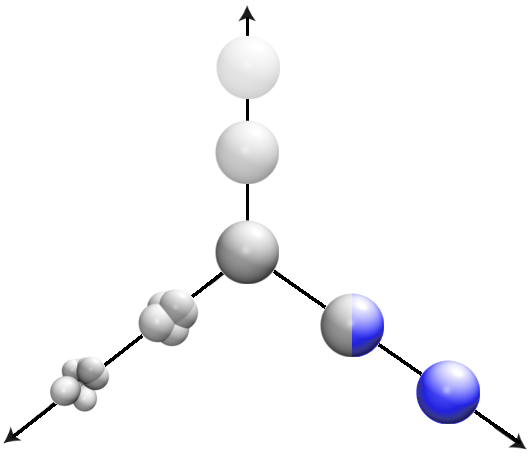
\includegraphics[width=0.6\textwidth]{anisotropyspace.png}
		\put(-133,212){(c)}
		\put(-260,22){(b)}
		\put(-15,20){(a)}
	\end{center}
	\caption[Anisotropy space]{An illustrated example of anisotropy space, with a hard sphere as the origin (``zero anisotropy'') and axes of (a) degree of hydrophobicity (Chapter~\ref{chap:janus}), (b) asphericity (Chapter~\ref{chap:aspherical}), and (c) softness (Chapter~\ref{chap:2dsoft}) (figure adapted from \citeauthor{glotzer}~\cite{glotzer}).}
\end{figure}


\section{Frequently-used numerical methods}
In this section, I will briefly describe two methods that are used frequently throughout this work.
First, a method by which crystalline order can be differentiated from the surrounding fluid will be discussed; next, an algorithm for calculating free energy differences with respect to a reference state is demonstrated.

\subsection{Measuring crystalline order using spherical harmonics: $\bar {\bf q}_l$}\label{sec:orderparamdesc}

The crystallinity of a system can be measured quantitatively using a local bond-order parameter originally introduced by Steinhardt \textit{et al.}~\cite{ronchetti} and used, for example, in~\cite{tenwolde,auer} and many others.
This method uses $l$-fold symmetric spherical harmonics to numerically differentiate crystal structures of that symmetry (most commonly, $l=6$, so that body-centered cubic [bcc], fcc, or hcp structures are detected) from the fluid.

For a given particle $i$, we define $q_l(i)$ as follows:
\begin{equation}
	q_l(i) = \left(\frac{4 \pi}{13} \sum_{m=-l}^{l} \left| q_{lm}(i) \right|^2\right)^{1/2} \,,
\end{equation}
where
\begin{equation}
	q_{lm}(i) = \frac{1}{N_b(i)} \sum_{j=1}^{N_b(i)}Y_{lm}\left(\hat{\bf r}_{ij}\right) \,.
\end{equation}
The sum in this equation is over all neighboring particles $j$ of particle $i$, where a particle is defined as ``neighboring'' if it is within some cutoff $r_q$ of particle $i$; $N_b(i)$ is the number of such neighboring particles to particle $i$.
$Y_{lm}\left(\hat{\bf r}_{ij}\right)$ is the $m$-component spherical harmonic evaluated for the normalized vector $\hat{\bf r}_{ij}$ from particle $i$ to particle $j$.

This parameter, $q_l(i)$, is sensitive to the degree of orientational correlations between vectors joining neighboring particles -- in a fluid, there are no preferred orientations and so the correlations decay rapidly, whereas in a crystal, the vectors are strongly correlated.
We can thus calculate a quantitative measure of the degree of crystallinity, and define two particles as ``connected'' within a crystalline structure if the correlation between neighboring particles,
\begin{equation}
	{\bf q}_l(i)\cdot{\bf q}_l(j) = \sum_{m=-l}^l q_{lm}(i) \cdot q_{lm}^*(j) \,,
	\label{eq:orderparam}
\end{equation}
is greater than some cutoff value $q_{\textrm {cut}}$.
Alternatively, the values of ${\bf q}_l(i) \cdot {\bf q}_l(j)$ can be averaged, for each particle $i$, over all neighbors $j$, yielding a single value $\bar q_l(i)$ -- comparing the result to a cutoff $q_{\textrm {cut}}$ allows particle $i$ to be defined as ``crystalline'' or ``non-crystalline.''
The number of connected particles to particle $i$ is denoted $N_X(i)$.
Figure~\ref{fig:q6dist} shows distributions of $q_6$, $q_4$, and $N_X$ values in liquid, bcc, and fcc systems, in order to illustrate the power of these measures for delineating crystalline vs. noncrystalline systems.

\begin{figure}
	\begin{center}
		\subfloat[]{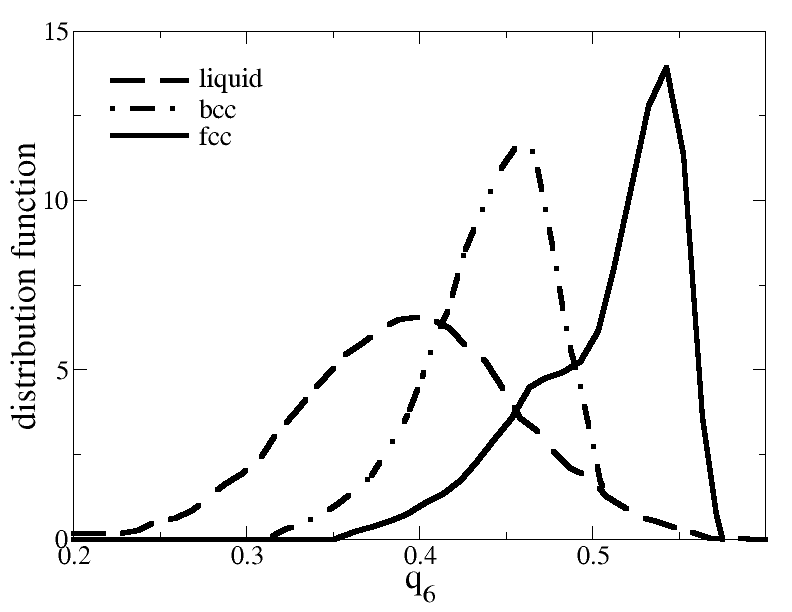
\includegraphics[width=0.6\textwidth]{q61.png}\label{q61dist}}

		\subfloat[]{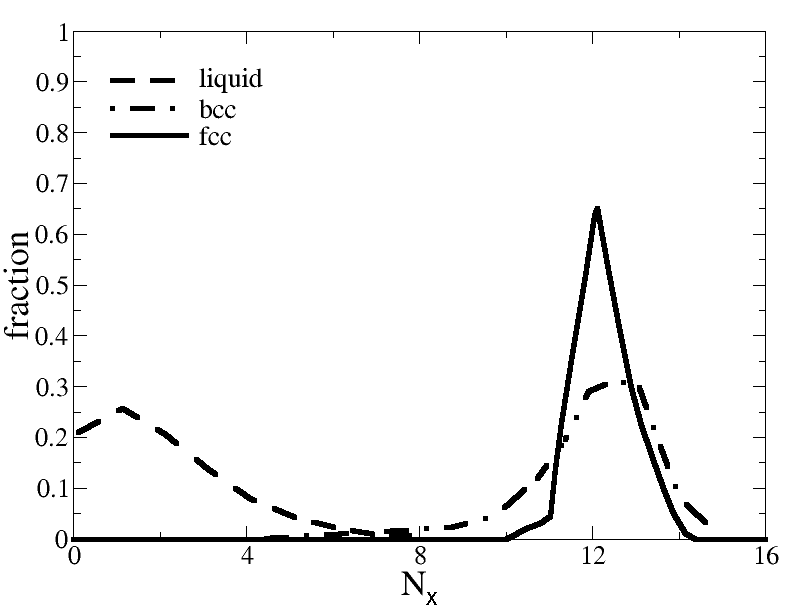
\includegraphics[width=0.6\textwidth]{q62.png}\label{q62dist}}
	\end{center}
	\caption[The distribution of $q_6$ and $N_X$ for liquid, bcc, and fcc systems]{The distribution of~\subref{q61dist} $q_6$ and~\subref{q62dist} $N_X$ for liquid, bcc, and fcc systems (figures created from data in \citeauthor{tenwolde2}~\cite{tenwolde2}).  While the $q_6$ values are different for the three systems, note that the number of connections $N_X$ is the strongest distinguisher between crystalline and noncrystalline systems, due to the fact that it accounts for relative orientation between neighboring particles.}\label{fig:q6dist}
\end{figure}

This order parameter will be used extensively throughout this dissertation.
In most cases, the six-fold symmetric $q_6$ will be used; in Chapter~\ref{chap:pixel}, $q_4$ is used, and some comments will be presented on the use of $q_4$ and $q_6$ values to differentiate between crystals of four- and six-fold symmetry.

\subsection{Calculating free energies: thermodynamic integration}\label{sec:thermint}
It is often desirable to compute the free energy of a system with respect to some reference.
One method for doing so, and the one that will be used in this dissertation (particularly, Chapter~\ref{chap:brush}), is thermodynamic integration~\cite{FrenkelBook}.

The Helmholtz free energy, $F$, is related to the canonical partition function $Q$ as follows:
\begin{align}	
	F &= - k_{\textrm B} T \ln Q(N, V, T) \notag \\
	&\equiv -k_{\textrm B} T \ln \left(\frac{\int d {\bf{p}}^N d {\bf{r}}^N \exp\left[-\beta \mathcal{H}({\bf {p}}^N, {\bf {r}}^N)\right]}{\Lambda^{dN} N!}\right) \,,
\end{align}
where $\mathcal{H}$ is the Hamiltonian of the system; $\bf p$ and $\bf r$ are the momenta and positions of all particles in the system, respectively; $d$ is the dimensionality; $N$ is the number of particles; $V$ is the volume; $T$ is the temperature; and the thermal de Broglie wavelength $\Lambda \equiv \frac{h}{\sqrt{2 \pi m k_{\textrm B} T}}$.

Assume that we can write the potential energy in a three-dimensional system, $V_\lambda$, as a linear function of some coupling parameter $\lambda$, such that for $\lambda = 0$, $V_\lambda$ equals some reference potential $V_{\textrm {ref}}$, and for $\lambda = 1$, $V_\lambda$ equals the potential of interest $V$:
\begin{equation}
	V_\lambda = (1 - \lambda)V_{\textrm {ref}} + \lambda V = V_{\textrm {ref}} + \lambda(V - V_{\textrm {ref}}) \,.
\end{equation}

Then, for a given value of lambda, the partition function $Q(N, V, T, \lambda)$ is given by
\begin{equation}	
	Q(N, V, T; \lambda) = \frac{1}{\Lambda^{3 N} N!}\int{d {\bf {r}}^N e^{-\beta V_\lambda}} \,.
\end{equation}
The derivative of $F$ with respect to $\lambda$ can then be written
\begin{align}
	\left(\frac{\partial F(\lambda)}{\partial \lambda}\right)_{N, V, T} &= -\frac{1}{\beta} \frac{\partial}{\partial \lambda} \ln Q(N, V, T; \lambda) \notag\\
	%&= -\frac{1}{\beta Q(N, V, T, \lambda)} \frac{\partial Q(N, V, T, \lambda)}{\partial \lambda} \notag\\
	&= \frac{\int{d {\bf {r}}^N \left(\frac{\partial V_{\lambda}}{\partial \lambda}\right)e^{-\beta V_\lambda}}}{\int{d {\bf {r}}^N e^{-\beta V_\lambda}}} \notag\\
	&\equiv \left<\frac{\partial V_\lambda}{\partial \lambda}\right>_\lambda \,,
\end{align}
where the notation $\left<...\right>_\lambda$ is used to denote the ensemble average for a system with potential energy function $V_\lambda$.

The energy difference between the system with the potential of interest $V$ and the reference system with potential $V_{\textrm {ref}}$ can then be found by integrating
\begin{equation}
	\Delta F \equiv F(\lambda = 1) - F(\lambda = 0) = \int_{\lambda = 0}^{\lambda = 1} d\lambda \left<\frac{\partial V_\lambda}{\partial \lambda}\right>_\lambda \,. \label{deltaF}
\end{equation}
Thus, the free energy difference $\Delta F$ can be calculated by integrating a derivative of the readily accessible quantity, the total potential, with respect to $\lambda$.
In practice, this is done by sampling at several values of $\lambda \in \left[0,1\right]$ and integrating numerically.

\section{Organization of this dissertation}

This dissertation is organized as follows.

In Chapter~\ref{chap:janus}, we discuss the self-assembly of particles with partially hydrophobic and partially hydrophilic surfaces, and determine the effect of the ratio of the two areas.
It is based on work published in~\cite{cacciuto}.


Chapter~\ref{chap:aspherical} presents studies of the thermodynamics of crystallization in systems of aspherical particles, and identifies order parameters via which the crystallization coexistence pressure can be predicted.
It is based on work published in~\cite{disorder1} and~\cite{disorder2paper}.

A study of the packing of soft particles in two dimensions is presented in Chapter~\ref{chap:2dsoft}.
A few different soft interaction potentials are considered and a wide variety of crystalline structures of different overall symmetry result.
It is based on work published in~\cite{2dsoftpaper}.

Chapter~\ref{chap:brush} contains the results of a study of two-component polymer brushes grafted to cylinders in alternating stripes.
The dependence of the free energy on stripe width and the lengths of the polymers is considered.
It is based on work published in~\cite{brushpaper}.

Finally, in Chapter~\ref{chap:pixel}, we present an algorithm for the reverse self-assembly problem; that is, the determination of an optimal interaction potential given a desired target crystal structure.
We speculate possible expansions of the method and present a new model for interparticle interaction that should allow a great deal of flexibility in such algorithms.
It is based on work published in~\cite{pixelpaper}.

\comment{
	Thus, in Chapter~\ref{chap:janus}, we focus on a specific system -- asymmetric Janus particles -- and study, in detail, the self-assembly pathway.
We find that the pathway is hierarchical; that is, assembly occurs via combination of mesostructures until a critical size is reached, rather than by sequential addition of nanoparticles to the aggregates.


In Chapter~\ref{chap:janus}, we study the self-assembly of a particular class of colloidal nanoparticles; in particular, so-called asymmetric Janus particles.
A Janus particle is an amphiphatic particle -- that is, a particle that has both a hydrophobic and a hydrophilic region on its surface -- which is divided in half between its two regions.
We generalize this to systems in which the ratio of hydrophobic to hydrophilic surface area varies between the extremes of isotropic hydrophobic and isotropic hydrophilic particles, and systematically describe the effect of this ratio on the self-assembly pathway and equilibrium self-assembled structure.

In Chapter~\ref{chap:pixel}, we approach the reverse self-assembly problem.
That is, whereas traditional self-assembly studies (including that described in Chapter~\ref{chap:janus}) are concerned with questions of the type, ``Given a specific interparticle interaction, into what structure will the system self-assemble?'', we describe an algorithm for answering the reverse (and much more difficult) question, ``Given a specific desired target self-assembled structure, what interparticle interactions will yield a system which will self-assemble into that structure?''
Our method is limited to interactions of a specific type, but the algorithm is in principle generalizable. 
we also describe a new model of interparticle interaction which, in combination with an optimized version of our algorithm, should be able to generate interparticle interaction geometries with a high degree of flexibility.

\section{Packing}
Problems of packing and space tiling have fascinated scientists for a very long time.
Kepler's 1611 essay {\it On the Six-cornered Snowflakes} is probably one of the earliest publications on the subject.
Here he conjectured that cubic close packing and hexagonal close packing are the most efficient ways to fill a space using equally sized spheres.
It wasn't until 1998 that Kepler's conjecture was finally announce to be proven (with 99\% degree of confidence) by Thomas Hales~\cite{Hales}.

At its most basic level, particle packing is a fundamentally similar process to self-assembly.
However, because interactions between particles are purely repulsive, they will not spontaneously without an external driving force; for example, applied pressure.
Nevertheless, even under an isotropic external pressure, the wide variety of possible particle geometries can lead to a great deal of variety in particle packing.

In Chapter~\ref{chap:aspherical}, we examine systems of hard, aspherical particles.
We demonstrate that the thermodynamics of self-assembly of a system of these aspherical particle (either a system of identical particles or a polydisperse system of different-shaped particles) is well-predicted by a simple relationship between the crystallization pressure and two measures of particle asphericity borrowed from other fields.

In Chapter~\ref{chap:2dsoft}, we shift focus to systems of soft particle in two dimensions and on the surface of a sphere.
Soft particles are particles with a finite interaction potential at zero distance; such particles exhibit a surprisingly large variety of ordered structures at equilibrium.
In particular, for a given temperature, some of the interaction potentials studied demonstrate reentrant melting, or even more exotic behavior such as periodic transitions between different crystalline forms of different symmetries.
A similar phenomenon is seen when the study is extended to small numbers of soft particles on the surface of a sphere; in contrast to the Thomson problem of electrons on a sphere~\cite{thomson}, the results are highly radius-dependent.

Finally, in Chapter~\ref{chap:brush}, we study the special case of packing where the external force driving packing is the binding of monomers in polymer chains attached to a cylindrical surface.
We study the free energy of two-component polymer brush systems in which polymers of different length are patterned in alternating stripes of specified widths on the surface of a cylinder.
We present the dependence of the free energy on the polymer lengths and stripe width and a qualitative explanation of its functional form.}


%\part{Title of Part}
%\chapter{Hierarchical Self-Assembly of Asymmetric Janus Particles}
\label{sec:corpus}
\chapter{Self-assembly of asymmetric Janus particles}
\label{chap:janus}
\section{Introduction}
Spontaneous assembly of components into large ordered aggregates is a ubiquitous phenomenon in nature, and is observed across all length scales. Aggregation of proteins into functional nanomachines~\cite{Alberts}, formation of viral capsids~\cite{Watson,Klug}, packing of phospholipids into biological membranes~\cite{Sackmann} and assembly of colloidal particles into macroscopic  crystals~\cite{Subramanian} are just a few manifestations of this fundamental process. Because of advances in particle synthesis~\cite{DeVries,Schnablegger,Hong,Weller,Hobbie}, it is now possible to produce colloidal particles that are anisotropic both in shape and surface chemistry, thus providing an unlimited variety of building blocks that can spontaneously assemble into an unprecedented number of structures holding promise for the development of materials with novel functional, mechanical, and optical properties.

\comment{Although the generic features of particle aggregation can be described, at least phenomenologically, in terms of simple thermodynamic arguments~\cite{Israelachvili,Zhang,Leckband,Nagarajan}, the details of the process are far from being understood. 
In fact, for self-assembly to take place, a very delicate balance between entropic and energetic contributions, coupled to a precise geometric character of the components, must be satisfied. In general, self-assembly is not to be expected unless a careful design of the building blocks has been performed beforehand,
and this has inspired a large body of work dedicated to gain insight into how the geometry of the interparticle interactions and the shape of the particles themselves  determine the dynamical pathway and structure they aggregate into.  The ultimate goal is to be able to gather a sufficient understanding of the forward self-assembly process to then be able to develop tools that will allow us to tailor interparticle interactions to target desired structures. With this in mind, there is a clear necessity  to explore a new dimension in the classical temperature/concentration phase diagrams: the geometry of the interactions (see reference~\cite{glotzer} for a recent perspective on the subject and a review of the relevant literature.)}

Janus particles are spherical colloidal particles the surfaces of which have one hydrophobic and one hydrophilic hemisphere.
In aqueous solution, the effect of this surface anisotropy is to introduce an attraction between hydrophobic hemispheres of neighboring particles and a simple hard-sphere repulsion between the hydrophilic ones.
Janus particles are important because they represent what is probably the simplest model for the study of the role of surface anisotropy in colloidal aggregation. 

The self-assembly pathway of Janus particles has been described in some detail~\cite{Hong2} both experimentally and numerically.  
What was found is a rich behavior in terms of both the dynamics of self-assembly, and the final structure of the aggregates.
Specifically, by tuning the repulsion between the hydrophilic hemispheres, one can drive the system into two distinct phases: one in which particles form a gas of small clusters composed of four to thirteen particles, and another, at large salt concentration (screening Coulombic interactions), in which particles organize into long, branched, worm-like structures formed by cooperative fusion of the small clusters.  
Such particles are a particular type of a wider class of patchy particles, the self-assembly of a wide variety of which has been studied previously~\cite{glotzer,sciortino}.

Inspired by these experimental results, in this paper we go one step further and explore the dynamics and structure formation of anisotropic amphiphatic particles.
While the dividing surface  between hydrophobic and hydrophilic regions in Janus particles is set at the equator, herein particles in which this boundary is located at an arbitrary latitude on the particle's surface are considered, and the self-assembly of these particles, as a function of the size of the hydrophobic region, is systematically studied.
We thus explore a key ``anisotropy dimension'' (as discussed in Section~\ref{sec:anisotropy}) as related to the self-assembly of these particles.

This system is quite interesting because one can easily predict the formation of a wealth of different structures  as a function of the location of the dividing surface. 
For instance, we know that when the hydrophobic  region covers a very small area, particles  can only assemble into dumbbells (pairs of particles with hydrophobic patches pointing toward each other). 
We know that when the dividing surface is placed to slightly larger values, so that more particles can share the same hydrophobic surface, particles condense into small stable  clusters.
We also know the structures resulting from self-assembly of Janus particles, and of course, in the limit  of full coverage, we recover an isotropic potential which is known to lead to the formation of a fcc crystal. 

Using this simple system we can systematically study the formation of aggregates whose structure ranges from zero dimensions (dumbbells and meso-particles) to three dimensions (fcc crystals), and we can analyze how  the specificity of the local interparticle interactions correlates to the final self-assembled structure and its dynamics.


\section{Simulation details}
The amphiphilic character of the particles studied herein is modeled via an interaction potential that depends on both the separation between particle surfaces and the angle between particle axes, so that a precise shape and extent of the interaction may be defined.  
Our choice of the interaction potential is inspired by the model introduced in~\cite{Hong2}, which has been used to analyze actual experimental data of Janus Particles.

The potential presented in~\cite{Hong2} was specifically tailored to describe the physical properties of Janus particles at different salt concentrations, $\rho_s$.
At low and intermediate salt concentrations,  the repulsion between the charged hemispheres constrains  particles to interact head-on, with angular deviations that depend in a nontrivial way on $\rho_s$.
However, the more interesting structure formation (worm-like clusters) appears at large salt concentrations, where the role of electrostatic interactions becomes negligible. 
In this limit, particles can freely rotate, once in contact, within the boundaries of the hydrophobic regions.  
These regions can therefore be appropriately described by a short-ranged, isotropic attractive potential that acts within the boundaries of that region. 
Similarly, the hydrophilic region is well-characterized by a simple short-ranged repulsive interaction. 

Because we desire to study the dynamics of self-assembly, molecular dynamics (MD) simulations were used.
MD simulations require smooth potentials (ensuring finite forces), and thus simple square-well potentials are not amenable to this type of simulation -- the potential used are essentially smoother versions of these simple square-well potentials.

The potential used in our paper reflects the phenomenological behavior described above and has the following form:
\begin{equation}
	V(r,\theta_1,\theta_2) = V_{\rm rep}(r) + V_{\rm att}(r)\phi(\theta_1)\phi(\theta_2)\,,
\end{equation}
where $r$ is the distance between particles, $\theta_1$ is the angle between the axis of particle 1 and the axis between particle centers, and $\theta_2$ is the analogous angle for particle 2.  
$V_{\rm rep}(r)$ is a symmetric repulsive interaction that accounts for the particle excluded volume, and has the form of a shifted-truncated  Lennard-Jones potential:
\begin{equation}
	V_{\rm rep}(r) = \begin{cases} 4\epsilon_0 \left[ (\frac{\sigma}{r})^{12} - (\frac{\sigma}{r})^{6} +\frac{1}{4}\right] & r \leq 2^{\frac{1}{6}}\sigma 
			\\ 0 & r > 2^{\frac{1}{6}}\sigma \end{cases}\,.
\end{equation}

$V_{\rm att}(r)$ accounts for the attraction between the hydrophobic \emph{surfaces} on the particles.
If $r_s = |r - \sigma |$ is the distance between the particle surfaces,
\begin{equation}
V_{\rm att}(r) = 4 \epsilon\Biggl[\left(\frac{\sigma/2}{r_s+\sigma/2\times2^{1/6}}\right)^{12}
\left.-2\left(\frac{\sigma/2}{r_s+\sigma/2\times2^{1/6}}\right)^6\right] \,,
\end{equation}
and it extends up to $r=1.5\sigma$. Finally,
$\phi\left(\theta\right)$ is a smooth step function that modulates the angular dependence of the potential, and 
is equal to 1 within the region $\theta \leq \theta_{\rm max}$ and decays  to 
zero following the expression $\cos^2\left(\pi\left[\frac{\theta-\theta_{\rm max}}{2\theta_{\rm tail}}\right]\right)$ at the tail
of the angular range, i.e when $\theta_{\rm max}\leq\theta\leq\theta_{\rm max}+\theta_{\textrm{tail}}$ 
(with $\theta_{\rm tail}=10^{\circ}$). This particular value of $\theta_{\textrm{tail}}$ has been selected to generate a sufficiently smooth potential at the Janus interface to allow MD simulation with reasonable time steps.
See Figure~\ref{fig:phi} for an illustration of $\phi\left(\theta\right)$.
\begin{equation}
	\phi\left(\theta\right) = \begin{cases} 
		1 & \theta < \theta_{\textrm{max}} \\ 
		\cos^2\left(\pi\left[\frac{\theta-\theta_{\textrm{max}}}{2\theta_{\textrm{tail}}}\right]\right) & \theta_{\textrm{max}} \leq \theta \leq \theta_{\textrm{max}}+\theta_{\textrm{tail}} \\ 
		0 & \textrm{otherwise} 
	\end{cases}
\end{equation}

\begin{figure}
	\begin{center}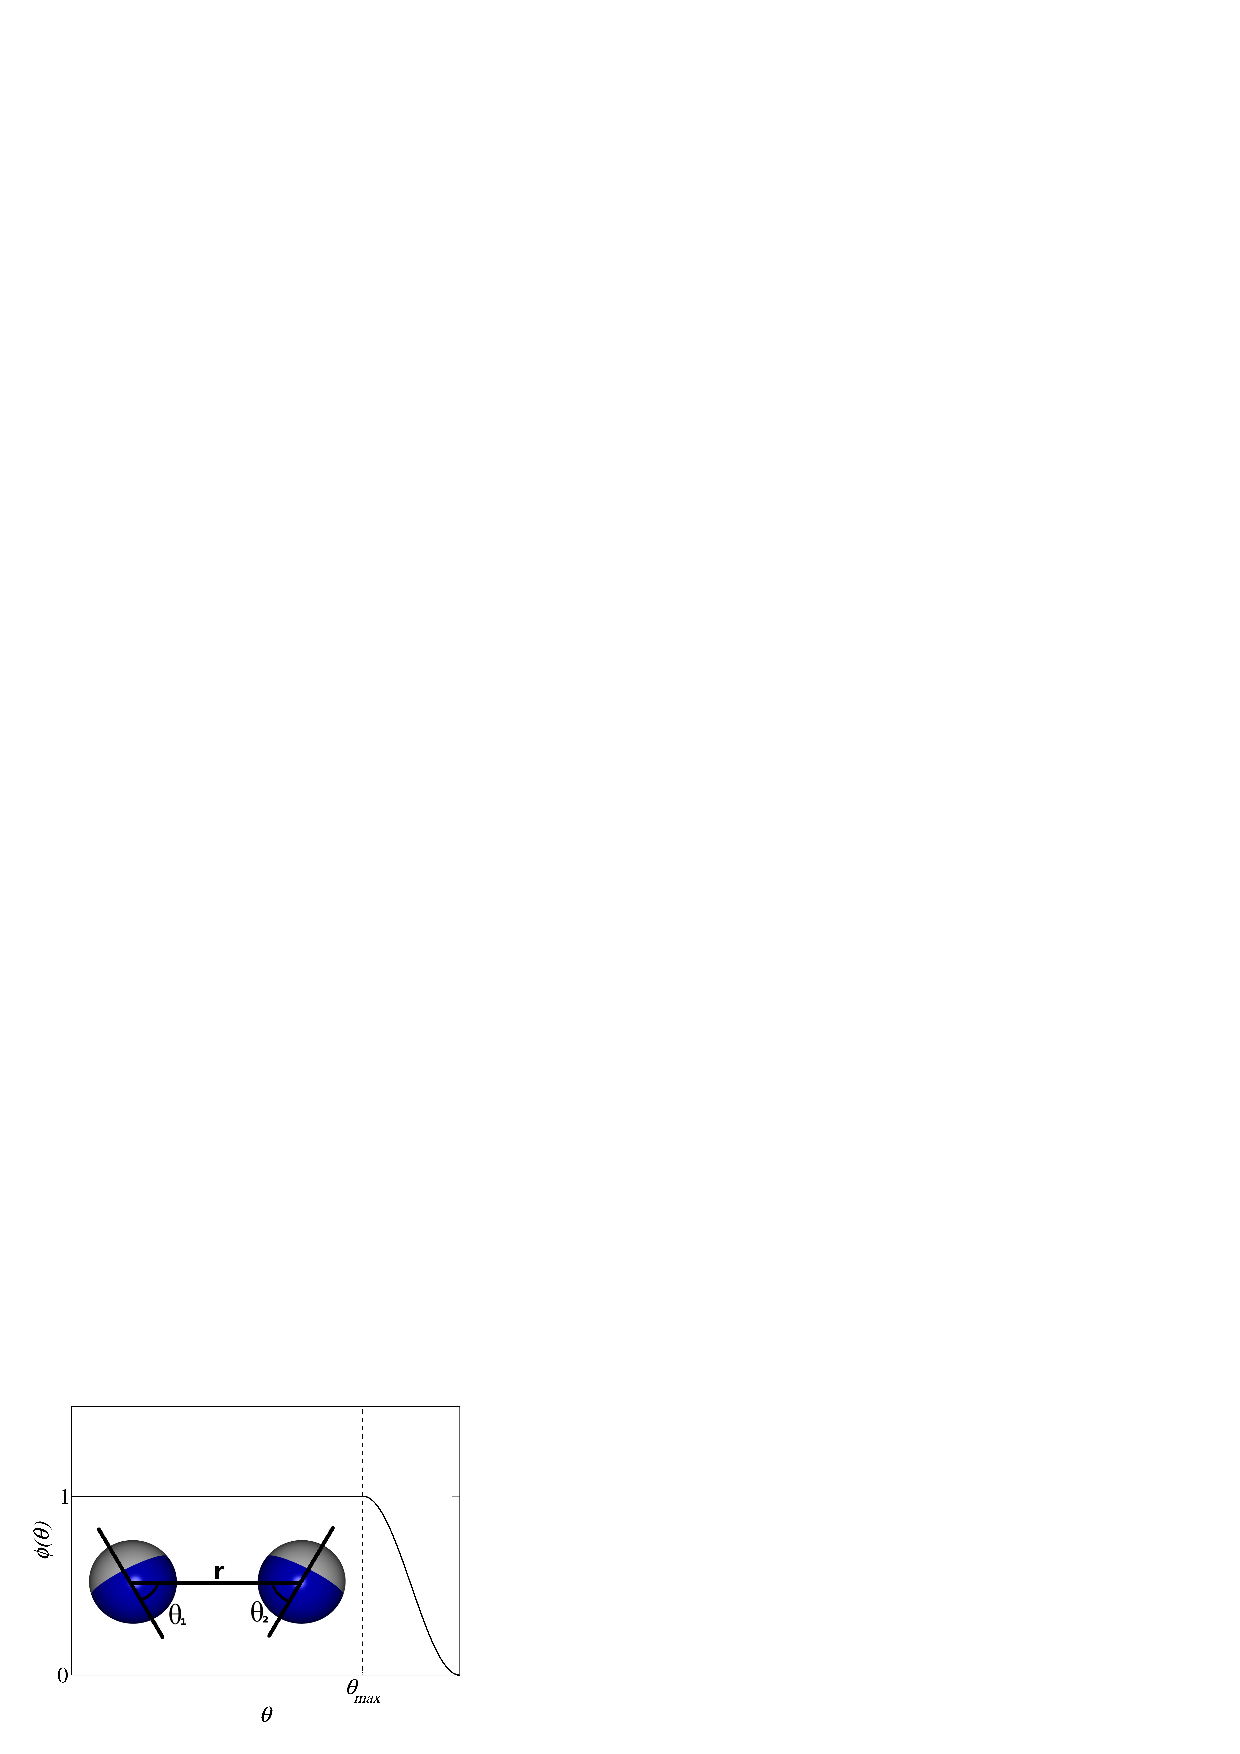
\includegraphics[width=0.6\textwidth,clip]{janus/phiwithimage}\end{center}
	\caption[Angular dependence of the interparticle potential]{Sketch of the angular dependence of the inter-particle potential $\phi\left(\theta\right)$.  The dark side represents the hydrophobic region and the light side represents the hydrophilic.}\label{fig:phi}
\end{figure}
The parameters set in our model are compatible with colloidal particles of size 200--400 nm in aqueous solution kept at a salt concentration sufficiently large to screen the electrostatic repulsion between the hydrophilic regions of any two particles~\cite{Hong2}.

The system is evolved using molecular dynamics simulations with a Langevin thermostat at constant room temperature, $T$, in a cubic box with periodic boundary conditions.
Our system contains $N=10^3$ particles kept at a constant volume fraction $\phi=0.01$.  
We have chosen this concentration because it is comparable with those used in experimental studies on Janus particles~\cite{Hong2}, so that our work could have a grounding experimental reference that our results could be compared to for $\theta_{\rm max}\simeq 90^{\circ}$.
Each simulation runs for  a minimum of $10^7$ steps with a time step $\delta t=0.001$. 
All quantities in this chapter (and throughout the rest of this dissertation) are expressed in standard dimensionless units.

\section{Structure formation}
Our goal is to understand how particles condense into stable three-dimensional aggregates via the process of self-assembly, and how the specificity of the  geometry of the interaction is reflected in the final structure.
Figure~\ref{fig:patchsize} reports one of the main results of our simulations.  
It shows a diagram indicating the lines in $\theta_{\textrm{max}}$-$\varepsilon$ space separating the different self-assembled structures obtained, with a typical resolution of one degree for $\theta_{\rm max}$, and 0.1$k_{\rm B}T$ for the binding energy. 

\begin{figure}
	\begin{center}
	\subfloat{
       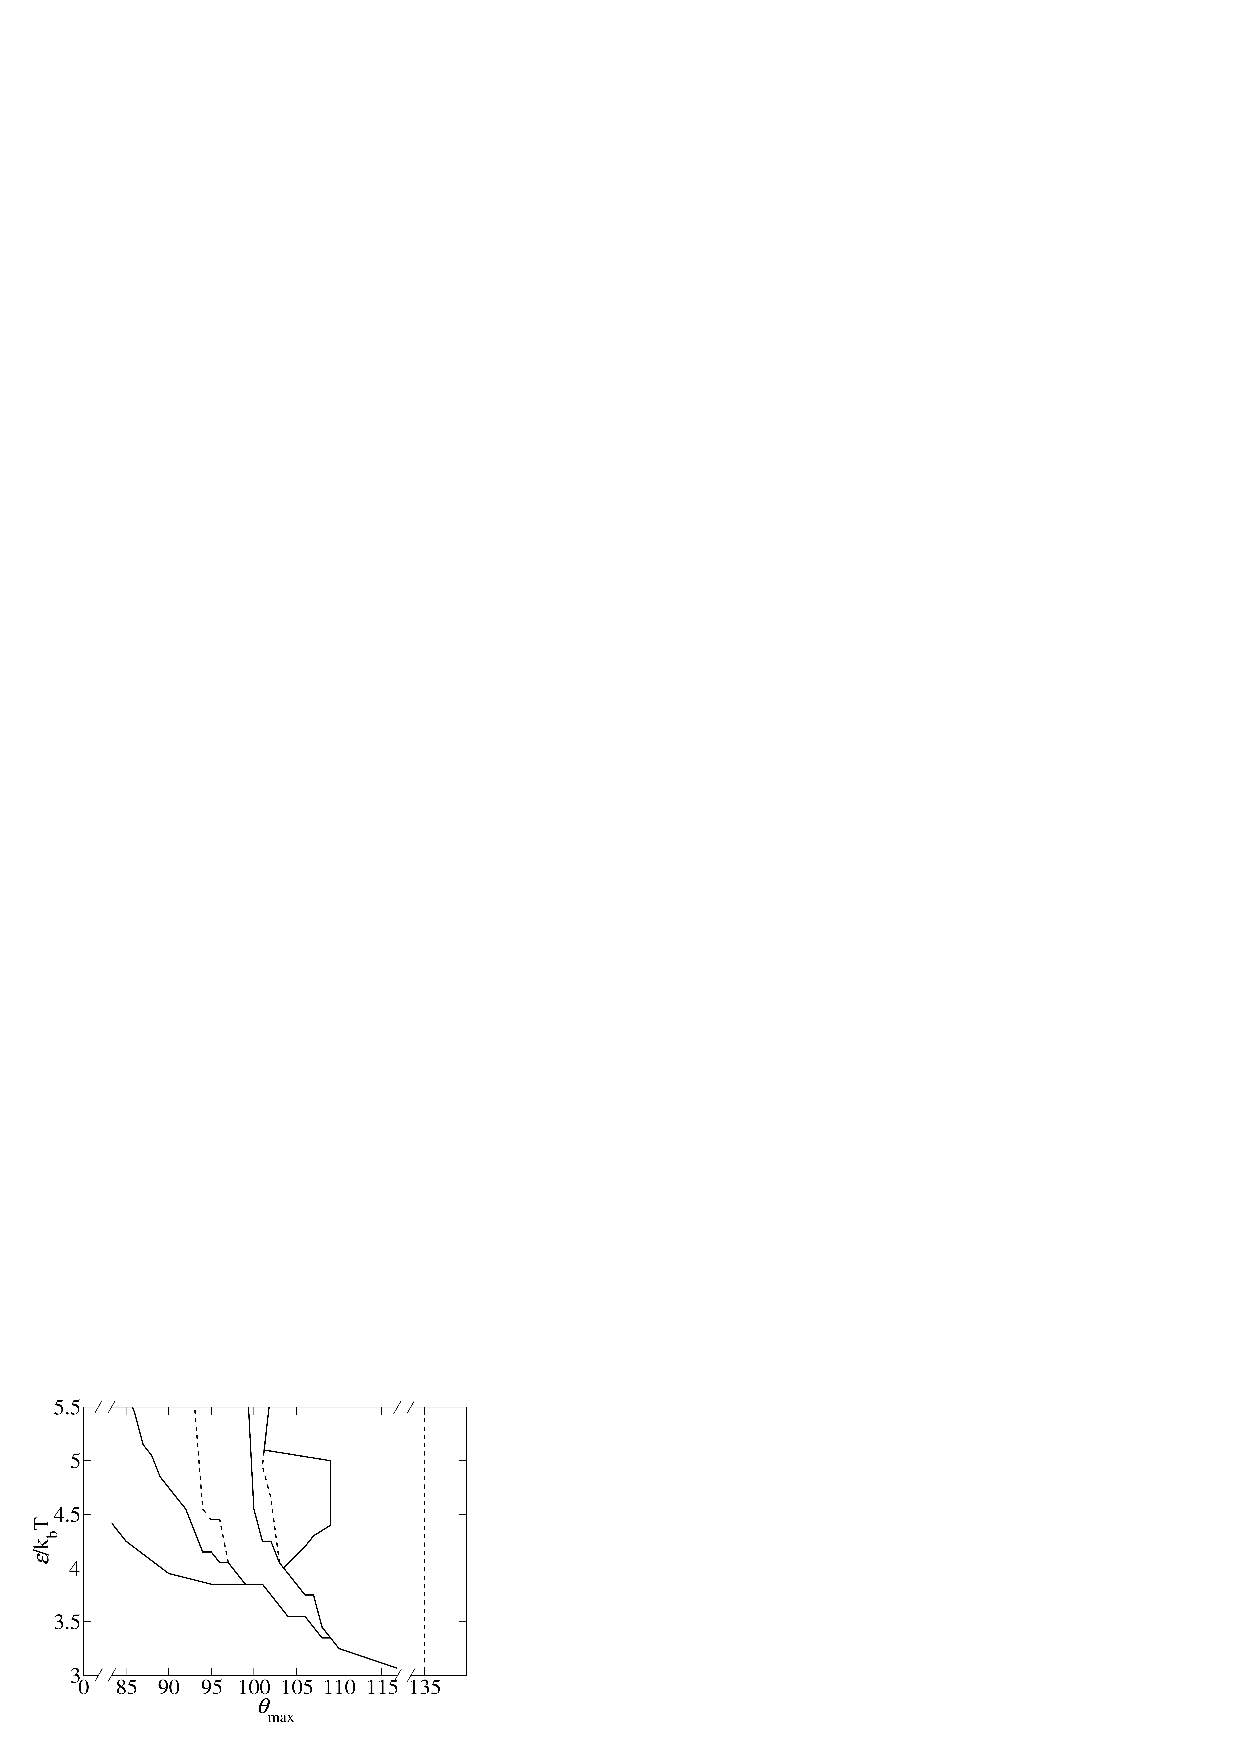
\includegraphics[width=3.28in,clip]{janus/phases2}
       \put(-150,50){\bf{gas}}
       \put(-180,110){\bf{\subref{fig:meso}}}
       \put(-170,150){\bf{\subref{fig:patch90}}}
       \put(-140,135){\bf{\subref{fig:patch95}}}
       \put(-105,160){\bf{\subref{fig:patch100}}}
       \put(-106,163){\vector(-1,0){10}}
       \put(-105,120){\bf{\subref{fig:patch105}}}
       \put(-60,120){\bf{\subref{fig:patch110}}}
       \put(-22,130){\bf{\subref{fig:patch180}}}
   }
  
   \setcounter{subfigure}{0}
   \subfloat[]{
       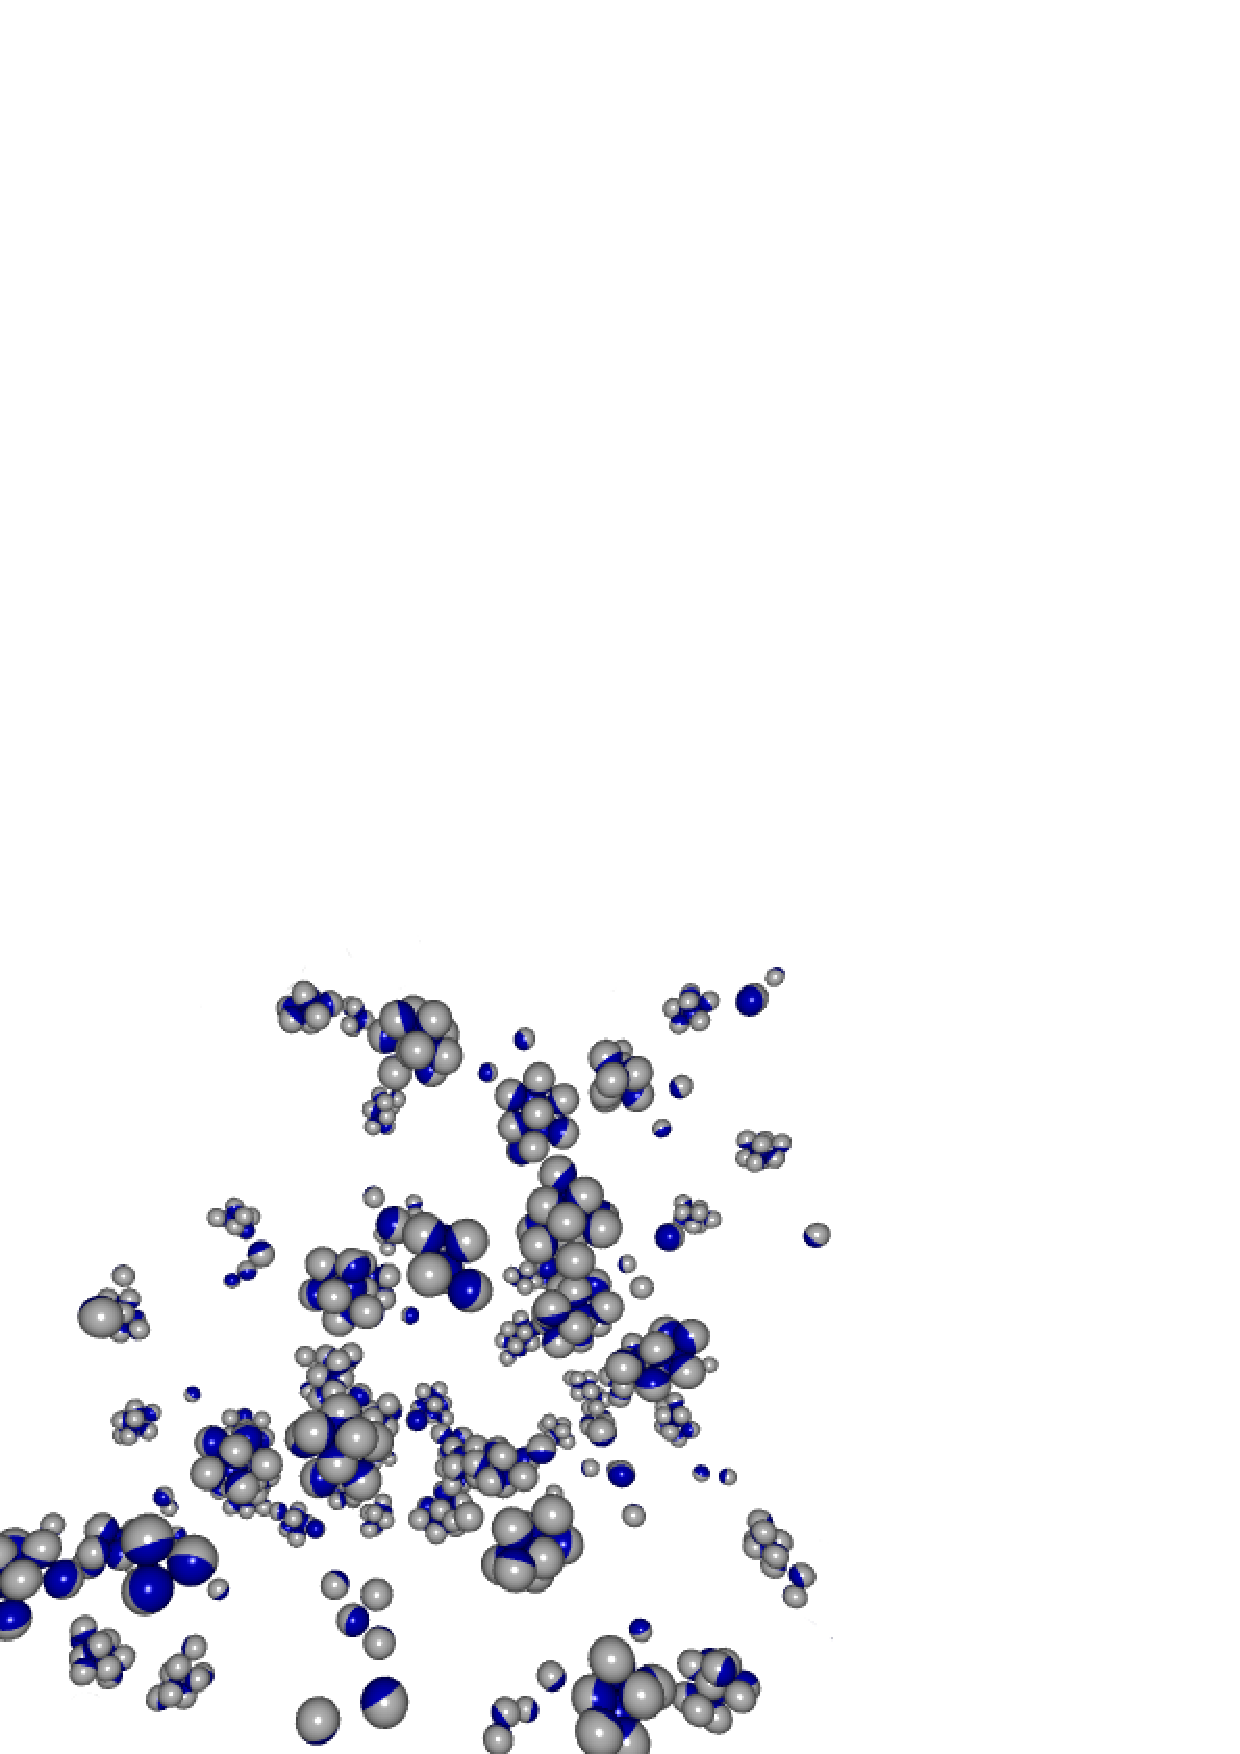
\includegraphics[width=1.23in,clip]{janus/meso}\label{fig:meso}
   }
   \subfloat[]{
	   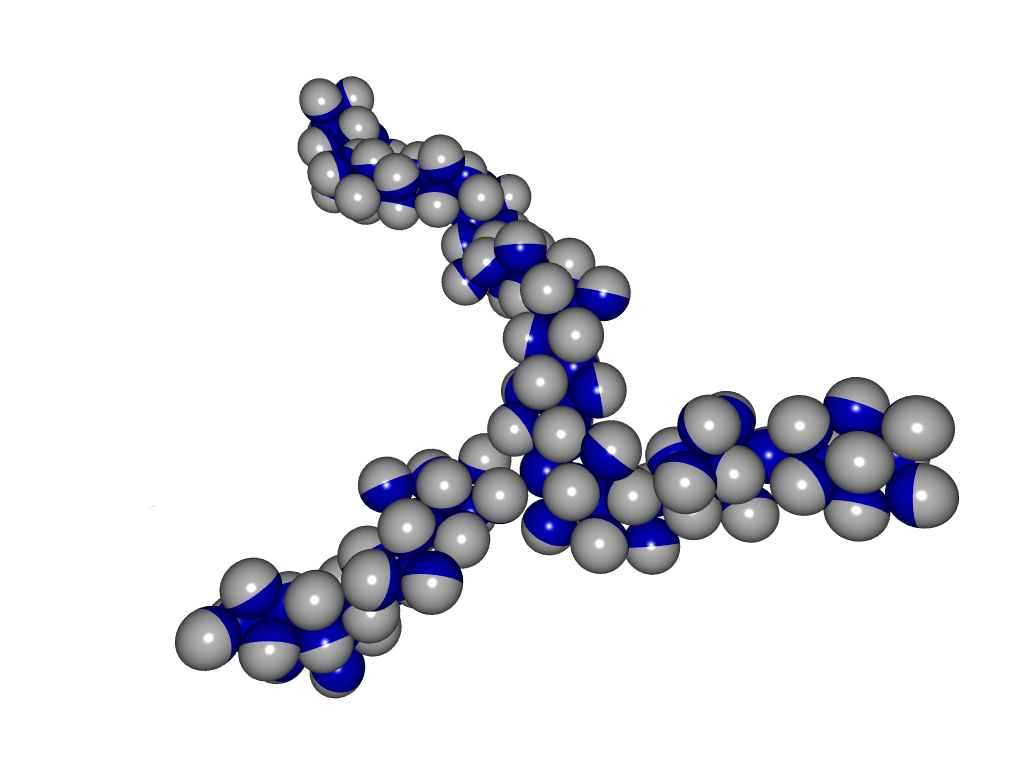
\includegraphics[width=1.23in,clip]{janus/90}\label{fig:patch90}
   }
   \subfloat[]{
       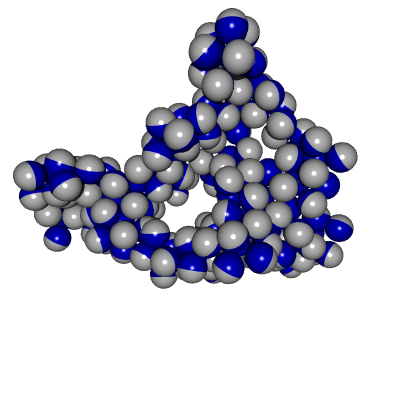
\includegraphics[width=1.23in,clip]{janus/95}\label{fig:patch95}
   }
   \subfloat[]{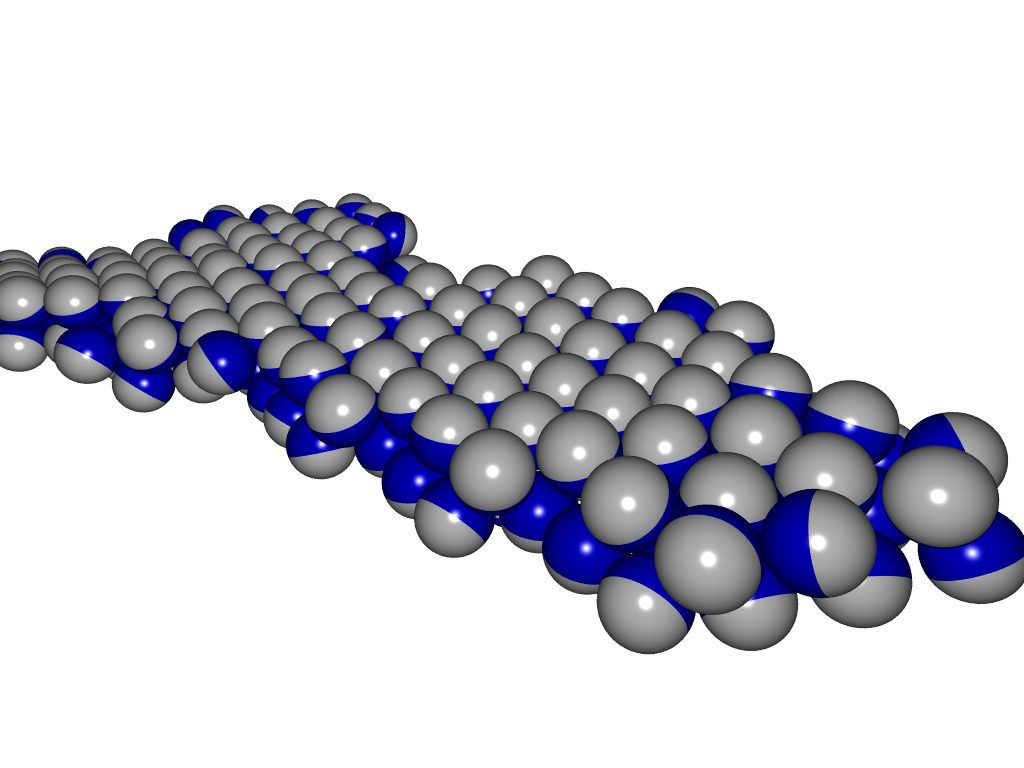
\includegraphics[width=1.23in,clip]{janus/100}\label{fig:patch100}
   }
   
   \subfloat[]{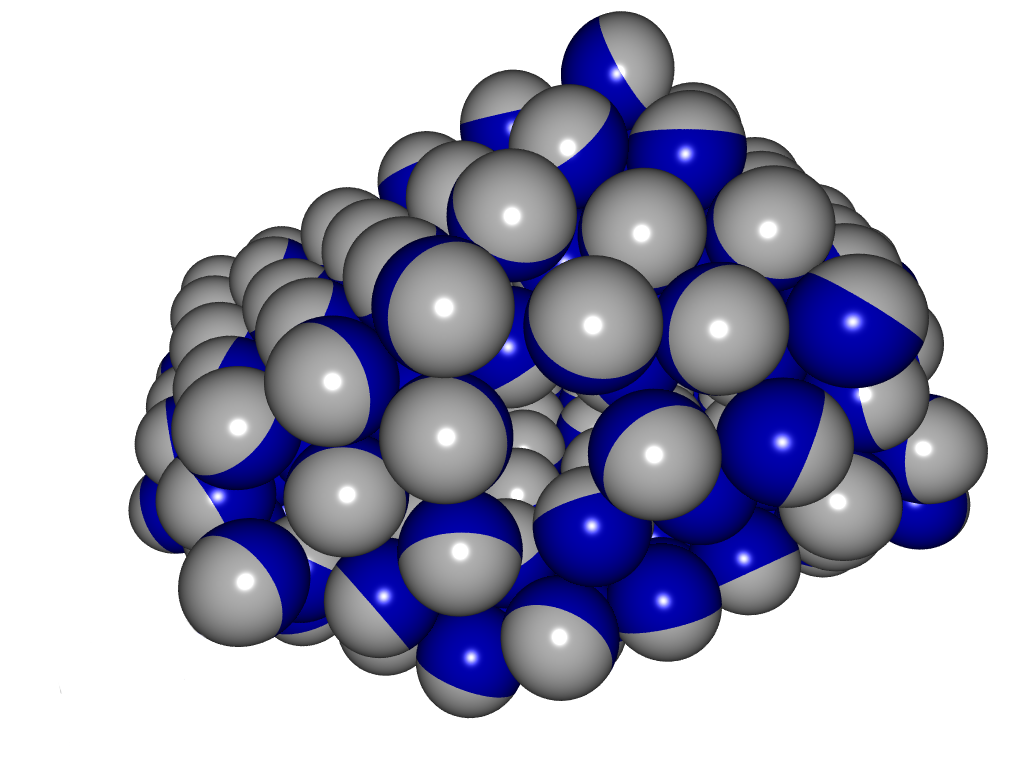
\includegraphics[width=1.23in,clip]{janus/105}\label{fig:patch105}
   }
   \subfloat[]{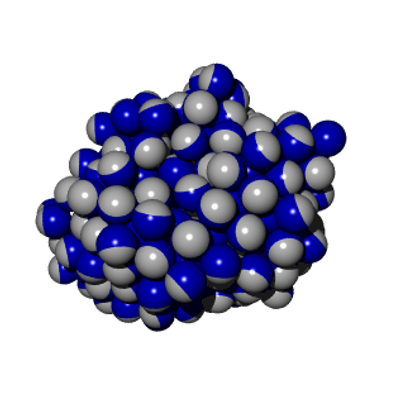
\includegraphics[width=1.23in,clip]{janus/115}\label{fig:patch110}
   }
   \subfloat[]{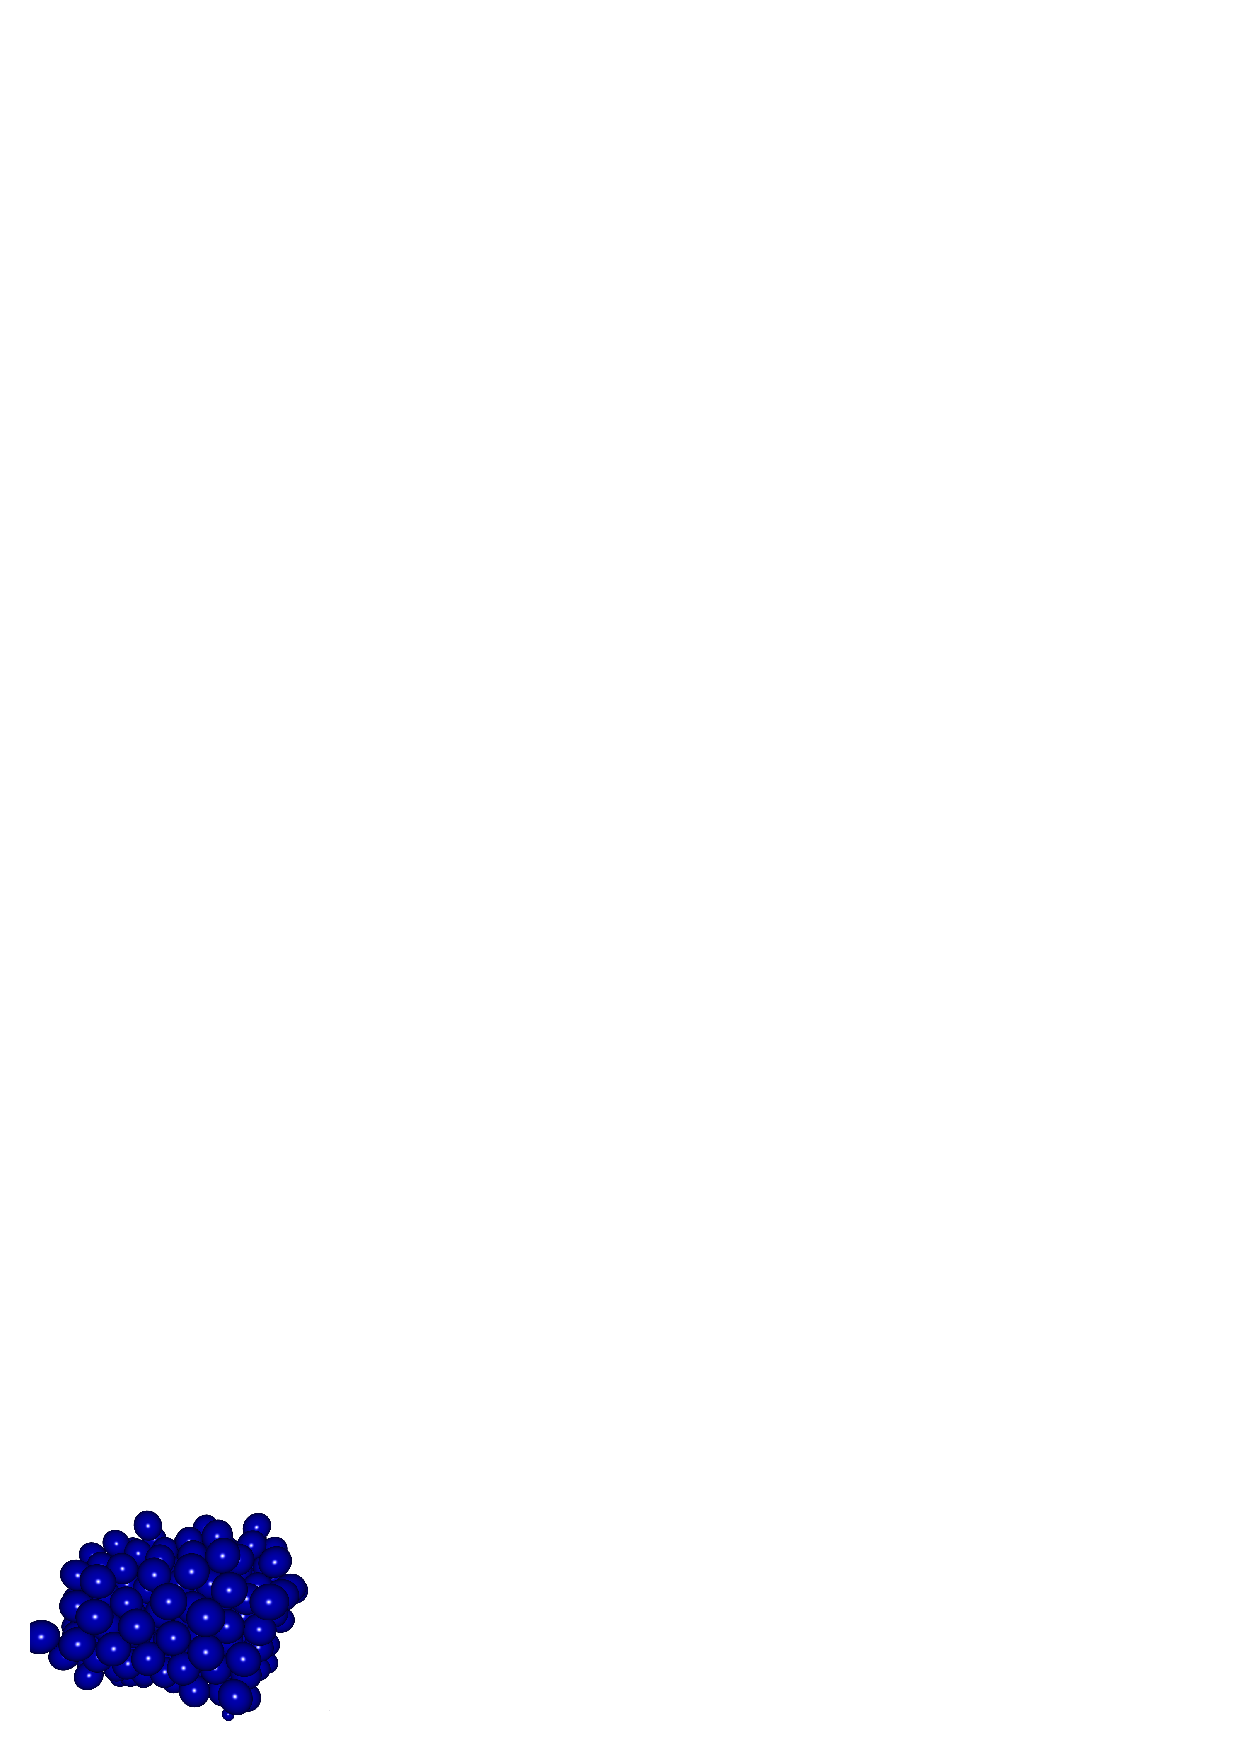
\includegraphics[width=1.23in,clip]{janus/180}\label{fig:patch180}
   }
   \end{center}
   \caption[Phase diagram for amphiphilic colloidal particles]{\label{fig:patchsize}Self-assembly diagram of amphiphilic colloidal particles as a function of binding energy 
   $\varepsilon$ and size of  hydrophobic region  $\theta_{\rm max} $. Region~\subref{fig:meso} is populated by small micelle-like clusters containing
   four to thirteen particles. Region~\subref{fig:patch90} contains branched  worm-like aggregates. In region~\subref{fig:patch95} we find self-connected worm-like aggregates.
   Region~\subref{fig:patch100} delimits flat hexagonal bilayers. In region~\subref{fig:patch105} we find faceted hollow cages. Region~\subref{fig:patch110} is populated by fluid amorphous 
   aggregates. Finally, in region~\subref{fig:patch180} we find large clusters with fcc order.}
\end{figure} 

As expected, a rich variety of structures arises depending on the position of the dividing surface $\theta_{\rm max}$, and particles' binding energy, $\varepsilon$. 
Notice that, consistent with numerical simulations on self-assembly of viral capsids~\cite{chandler} and chaperonins~\cite{geissler}, intermediate ordered  aggregates are extremely sensitive to the size of the hydrophobic region and self-assembly occurs in a very narrow region.

At low binding energy the system is in a gas state.
For small values of $\theta_{\rm max}$ and moderate values of $\varepsilon$ (Figure~\ref{fig:meso}) particles aggregate into small  clusters of 4 to 13 particles (mesoparticles)  {including icosahedral structures like those seen in \cite{wilber}}.
For $\theta_{\rm max} \sim 90^{\circ}$, self-assembly yields worm-like extended structures (Figure~\ref{fig:patch90}), as has been observed previously for Janus spheres~\cite{Hong2}. 
As the angular location of dividing surface between the hydrophobic and hydrophilic regions region increases from $90^{\circ}$ to $180^{\circ}$  we find, in order of appearance,  self-connected worm-like structures (Figure~\ref{fig:patch95}), flat-crystalline bilayers  (Figure~\ref{fig:patch100}), faceted hollow cages (Figure~\ref{fig:patch105}) (similar to structures seen in the self-assembly of cone-shaped particles~\cite{glotzer6,glotzer3}, yet not restricted to specific magic numbers of particles), amorphous fluid  blobs (Figure~\ref{fig:patch110}), and finally fcc crystals (Figure~\ref{fig:patch180}).

\section{Self-assembly pathways}\label{sec:Ostwald}

Apart from the possible relevance of phases~\subref{fig:patch100} and~\subref{fig:patch105} for practical applications, we want to point out that none of these structures arises following a  simple particle-by-particle growth mechanism, but rather by  two-to-three step hierarchical self-assembly.
The first step typically involves the formation of   {more- or less-structured} mesoparticles (depending on $\theta_{\rm max}$). 
Next, small clusters organize into either  extended worm-like aggregates, which  then coalesce or deform to produce the final structure,  or into larger fluid clusters that, once beyond some threshold size, spontaneously organize into structured aggregates.

The dynamical pathway leading to structures in region~\subref{fig:patch90} is detailed in reference~\cite{Hong2}, but in short, these worm-like structures form by the successive fusion of oligomers from trimers to heptamers; the individual particles reorient and rearrange so that they can fit together in a lock-and-key fashion to maintain five-fold rings with hydrophobic regions pointed into the interior of the worm.

It is of particular interest to discuss in some detail the dynamical pathway of structure formation relative to phases~\subref{fig:patch95}, \subref{fig:patch100}, and~\subref{fig:patch105}  as they all form via a complex three-step mechanism.
Surprisingly, the common precursor  to all of them is the worm-like structure stable at $\theta_{\rm max}\simeq 90^{\circ}$.
Self-connected worm-like aggregates  are a consequence of the improved flexibility of the  worm-like structures. As $\theta_{\rm max}$ increases, so does the ability of particles to rotate about their axes. 
The net result is that the branching ends of the clusters bend back upon themselves and begin to connect, thus forming topologically nontrivial aggregates.

To quantify the statistical difference between the aggregates found in regions~\subref{fig:patch90} and~\subref{fig:patch95},we measure their average radius of gyration 
\begin{equation}R_{\rm G}=\left ( \frac{1}{N_c}\sum_{i=1}^{N_c} \left<({\bf{r}}_i-{\bf{r}}_{\rm cm})^2\right> \right )^{1/2} \,,\end{equation}
where $N_c$ is the number of particles in the cluster, ${\bf{r}}_i$ is the position of particle $i$, and ${\bf{r}}_{\textrm cm}$ is the position of the center of mass of the cluster,
as a function of cluster size. 

Results are shown in Figure~\ref{gyration}, and clearly indicate that when $\theta_{\rm max}$ is increased from region~\subref{fig:patch90} to~\subref{fig:patch95}, the typical aggregate becomes more compact, showing a significantly smaller exponential dependence on the number of particles.
The limited statistics for large clusters prevent us from making any meaningful estimate of the chains' size exponent.
However, note that a perfectly linear chain would show an exponent of $1$ and a perfectly spherical aggregate would show an exponent of $\frac{1}{2}$.
Thus, the decreasing exponential dependence indicates a transition from ``linear-like'' chains towards more ``cluster-like'' geometry.
\begin{figure}
	\begin{center}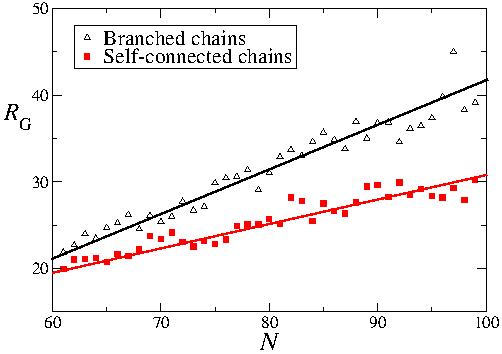
\includegraphics[width=0.6\textwidth]{janus/rg}\end{center}
		\caption[Radius of gyration vs. aggregate size]{Radius of gyration as a function of aggregate size $N$ for worm-like clusters in region~\subref{fig:patch90} and~\subref{fig:patch95} of Figure~\ref{fig:patchsize}. The lines are guides to the eye.}
		\label{gyration}

\end{figure}

We also measure the angular probability distribution function, $P(\cos(\alpha))$, between neighboring particles in  clusters containing at least 50 particles. 
Here $\alpha$ is defined as the angle between the particle axes; $\alpha = 0$ corresponds to particles with their patches pointing in the same direction, and $\alpha = \pi$ corresponds to particles pointing in opposite directions (which would be the case, for example, in two particles in a dumbbell configuration).

Figure~\ref{fig:p_of_alpha} shows  $P(\cos(\alpha))$ in regions~\subref{fig:patch90}, \subref{fig:patch95}, and~\subref{fig:patch100}.
$P(\cos(\alpha))$ shows a clear double peaked shape in region~\subref{fig:patch100}, indicating that most neighboring particles face either in the same direction (as would particles in a single monolayer sheet) or in the opposite direction (as would particles in the opposite monolayer of a bilayer structure), where the aggregates assume a planar bilayer configuration.

The more intriguing difference, however, is between region~\subref{fig:patch90} and~\subref{fig:patch95}, highlighted in the insert of the figure. 
Region~\subref{fig:patch90} is characterized by a peak at $\cos(\alpha)\sim -1$, and less distinguishable peaks at $\cos(\alpha)\sim \pm 0.74$ and  $\cos(\alpha)\sim -0.5$; overall there is a large probability for all possible orientations.
These data suggest that  branched worm-like aggregates have a roughly circular cross-section with particles oriented in a disordered fashion, but for a slight preference for a few selected angles (remnants of the mesoparticle structures from which they self-assembled), and an antiparallel neighbor opposite to most particles.

In contrast, region~\subref{fig:patch95} is characterized by a more distinct double-peaked function, with each peak close to $\pm 1$. 
This is consistent with a cross section that has flattened with respect to structures in region~\subref{fig:patch90}, and indicates that each branch of the aggregate is acquiring bilayer-like features.
The dashed line separating regions~\subref{fig:patch90} and~\subref{fig:patch95} shows where in the diagram the strings acquire sufficient flexibility to begin to form complex self-connected aggregates.   
\begin{figure}
	\begin{center}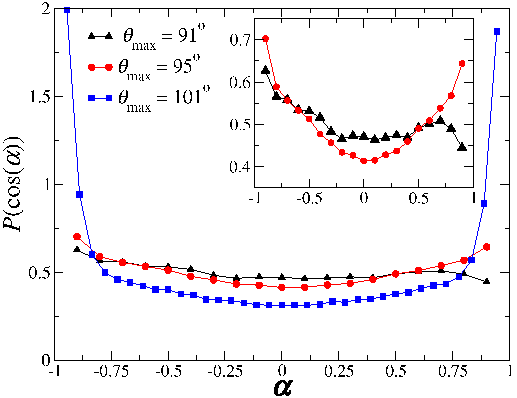
\includegraphics[width=0.6\textwidth]{janus/p_of_alpha}\end{center}
	\caption[Angular probability distribution function between neighboring particles]{Angular probability distribution function, $P(\cos(\alpha))$, between neighboring particles in  aggregates 	
	 containing at least 50 particles in region~\subref{fig:patch90} ($\theta_{\rm max}=91^{\circ}$), 
	 \subref{fig:patch95} ($\theta_{\rm max}=95^{\circ}$), and~\subref{fig:patch100} ($\theta_{\rm max}=101^{\circ}$), 
	 of the phase diagram. The insert highlights $P(cos(\alpha))$ 
	 in regions~\subref{fig:patch95} and~\subref{fig:patch100}. The data are averaged over 10 different clusters of each kind.}
	\label{fig:p_of_alpha}
\end{figure}

This observation is quite interesting when related to the dynamical pathway leading to phase~\subref{fig:patch100}.
Bilayers are formed by either coalescence of co-planar loops, as shown in Figure~\ref{fig:loops}, or by branch alignment.
This transition  occurs at $\theta_{\rm max}\simeq 110^\circ$, and it is driven by  the large energy gain attained by the aggregates when each particle surrounds itself with the suddenly increased number of neighbors compatible with the enlarged hydrophobic region; $110 ^\circ$ is roughly the value of $\theta_{\rm max}$ at which neighboring particles in a flat monolayer have a sufficiently favorable free energy to stabilize that geometry.
This transition is quite sharp and represents a beautiful example of how a very small perturbation of the geometry of the local interaction can lead to completely different macroscopic structures.

\begin{figure}
\begin{center}
	\renewcommand{\thesubfigure}{\arabic{subfigure}}
	\subfloat[]{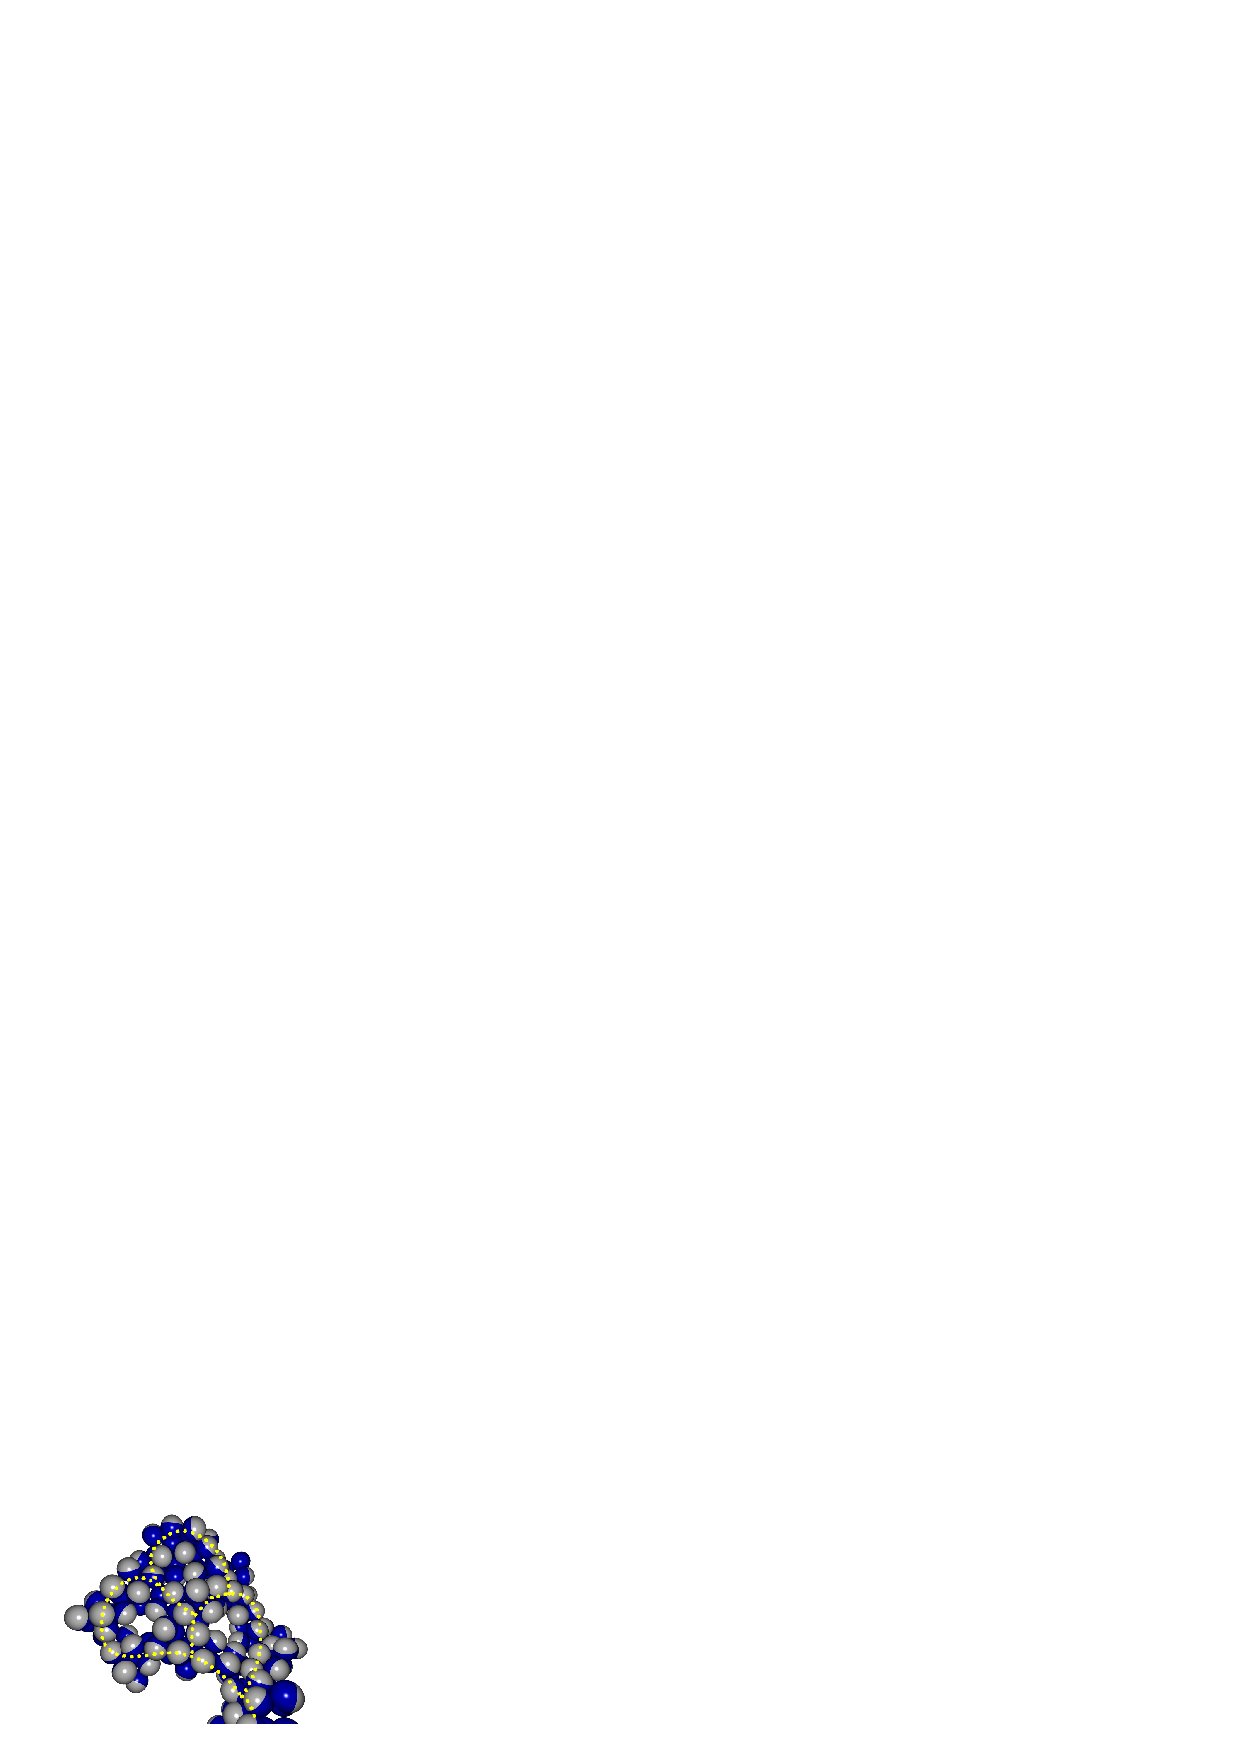
\includegraphics[width=0.45\textwidth]{janus/data1b}}
	\subfloat[]{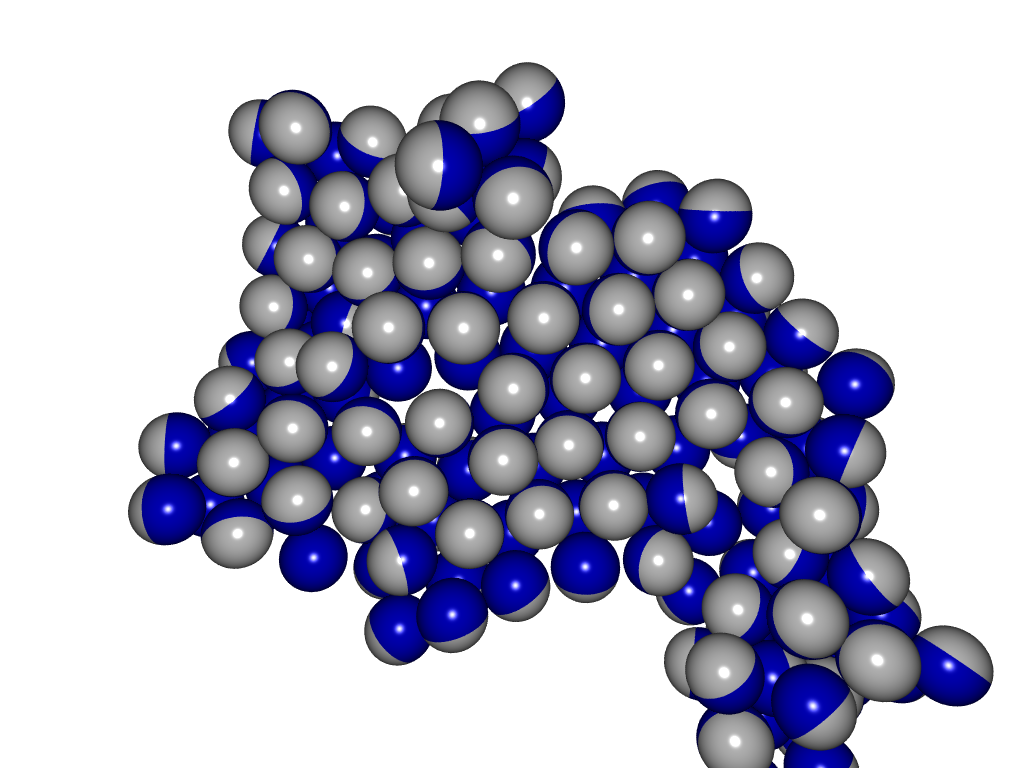
\includegraphics[width=0.45\textwidth]{janus/data2}}

	\subfloat[]{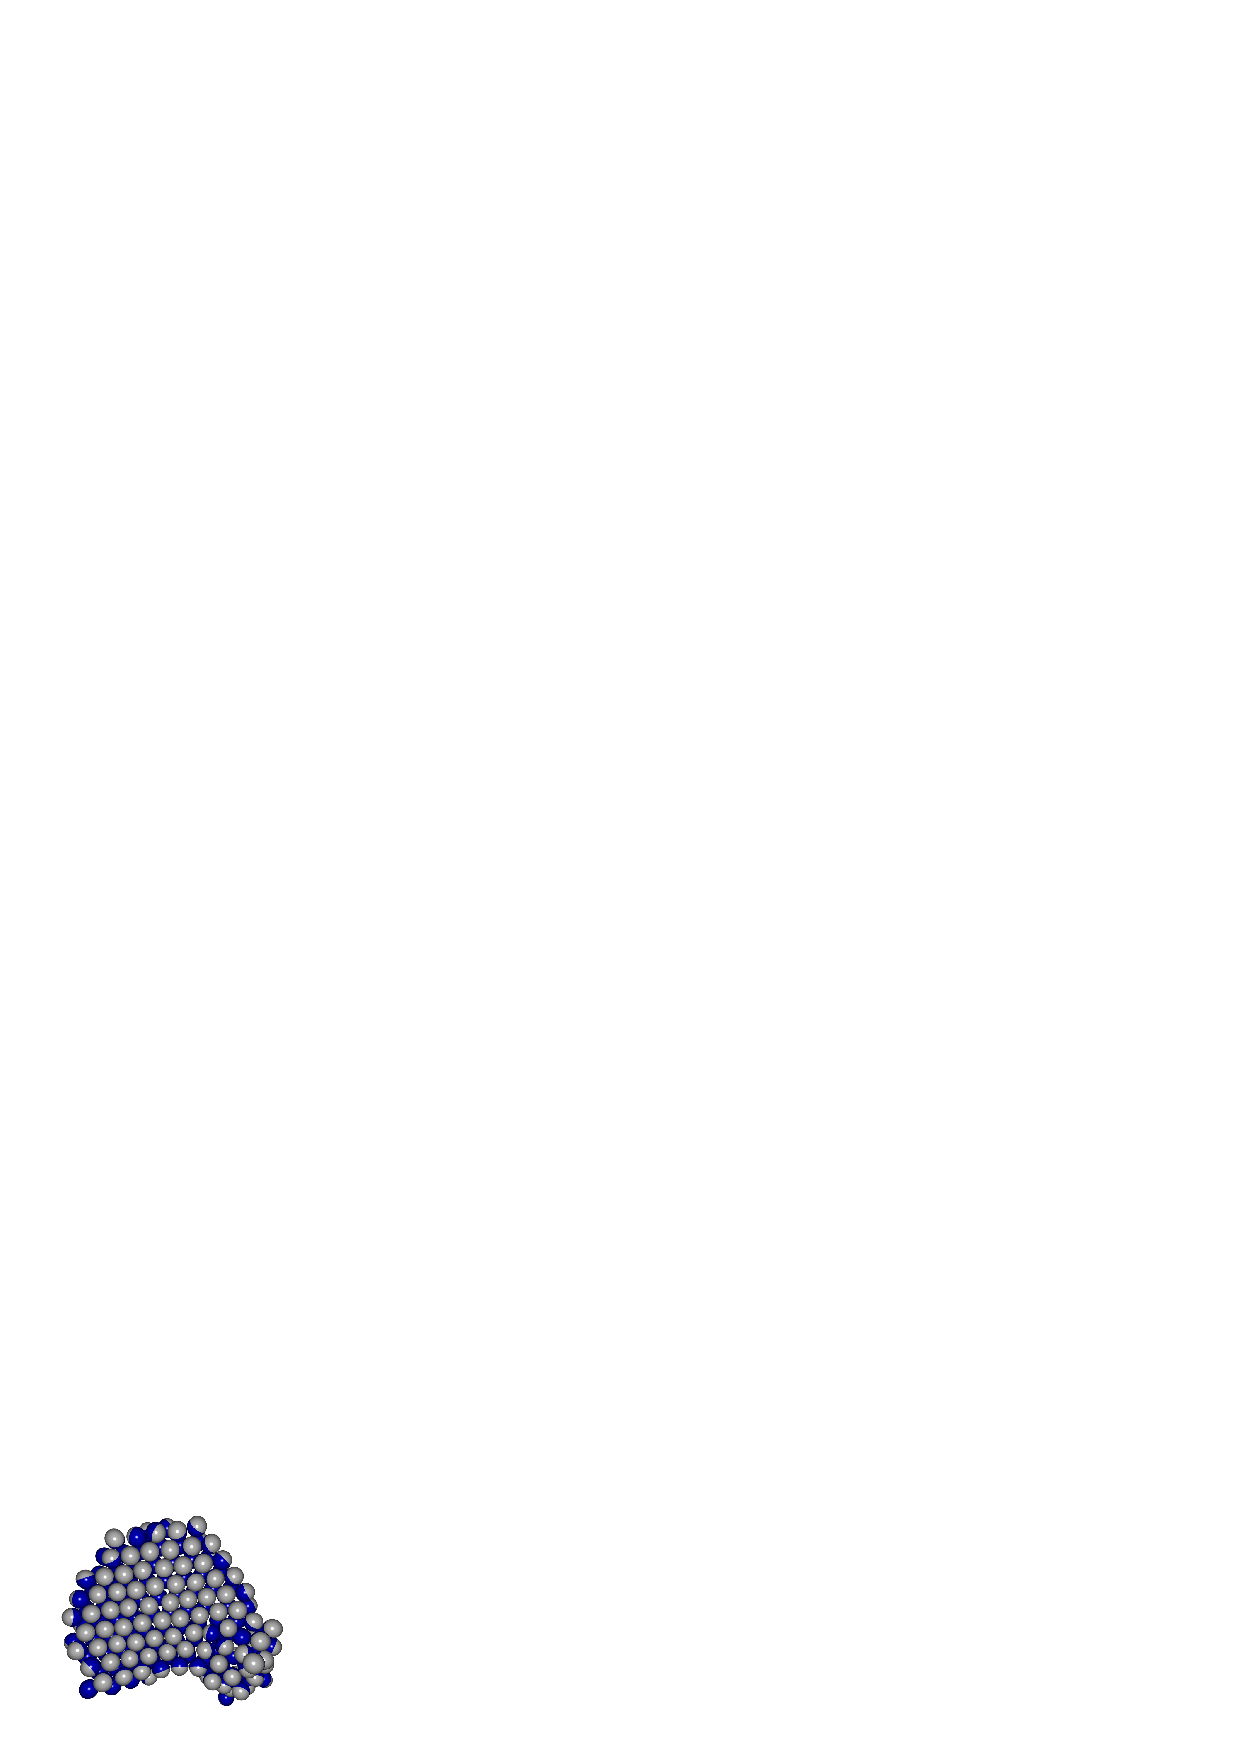
\includegraphics[width=0.45\textwidth]{janus/data3}}
\end{center}
		\caption[Snapshots of bilayer formation]{Sequence of three snapshots from our simulations showing the mechanism of  bilayer formation via coalescence of three coplanar loops.}
		\label{fig:loops}
\end{figure}

Finally, formation of finite-sized, faceted capsids does not occur by self-assembly of  misoriented, disjoined bilayers, but via a mechanism which, once again,  involves multiple steps. 
As we increase the size of the particles' hydrophobic region, short worm-like clusters, which are now very flexible (owing to the highly permissive large hydrophobic patches), immediately fold onto themselves to form small, amorphous fluid blobs. 
We find that these blobs tend to remain fluid-like, whereas larger ones morph into faceted  cages via a mechanism similar to that described for the formation of bilayers.
Fusion of fluid blobs, as illustrated in Figure~\ref{fig:snapshots}, is the main mechanism through which large blobs, which eventually turn into  faceted cages, are generated.

The dashed line between regions~\subref{fig:patch100} and~\subref{fig:patch105} indicates the onset of cage formation; however, a non-negligible number of planar aggregates are found to coexist with the faceted cages in region~\subref{fig:patch105}. 
It is worth stressing that these faceted cages can be considered as colloidal analogs of the lipid vesicles discussed previously; they are hollow,  their inner walls are hydrophilic, and one could in principle consider using them as possible drug carriers, with edges and corners presenting convenient locations for outer surface tagging.
Furthermore, while a systematic study of their thermodynamics has not been performed, it would be expected to have features consistent with the calculation of the critical micellar concentration given in Section~\ref{sec:cmc}.

\begin{figure}
	\begin{center}
	\renewcommand{\thesubfigure}{\arabic{subfigure}}
	\subfloat[]{
		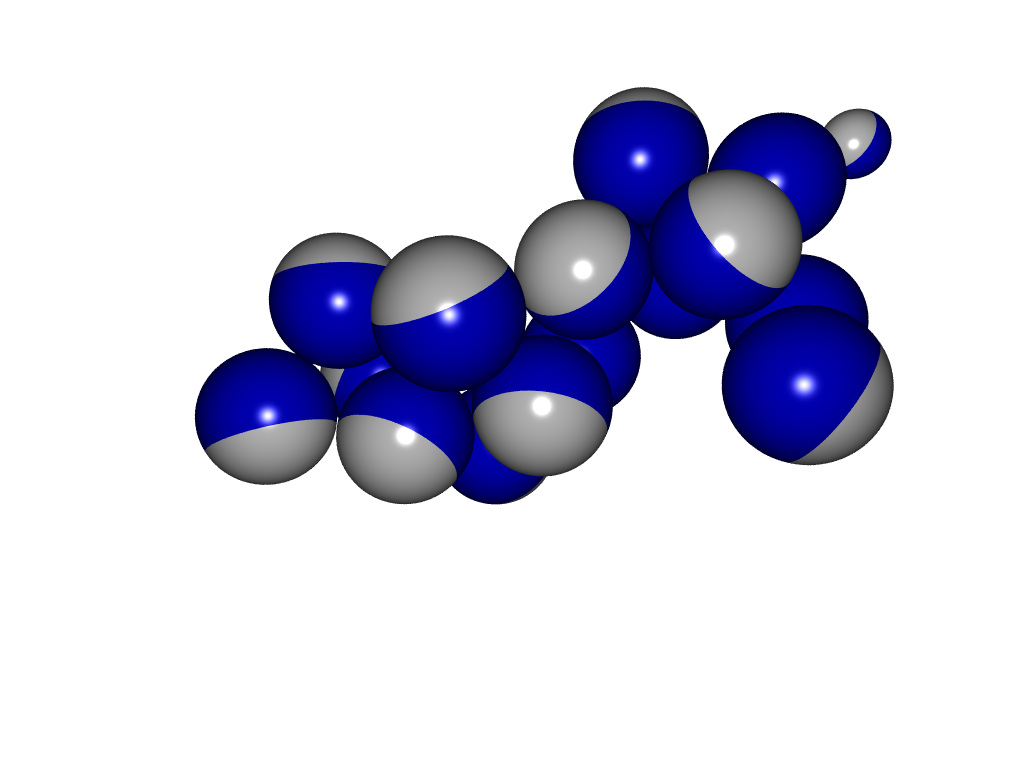
\includegraphics[width=0.45\textwidth]{janus/shota}\label{fig:shota}
	}
	\subfloat[]{
		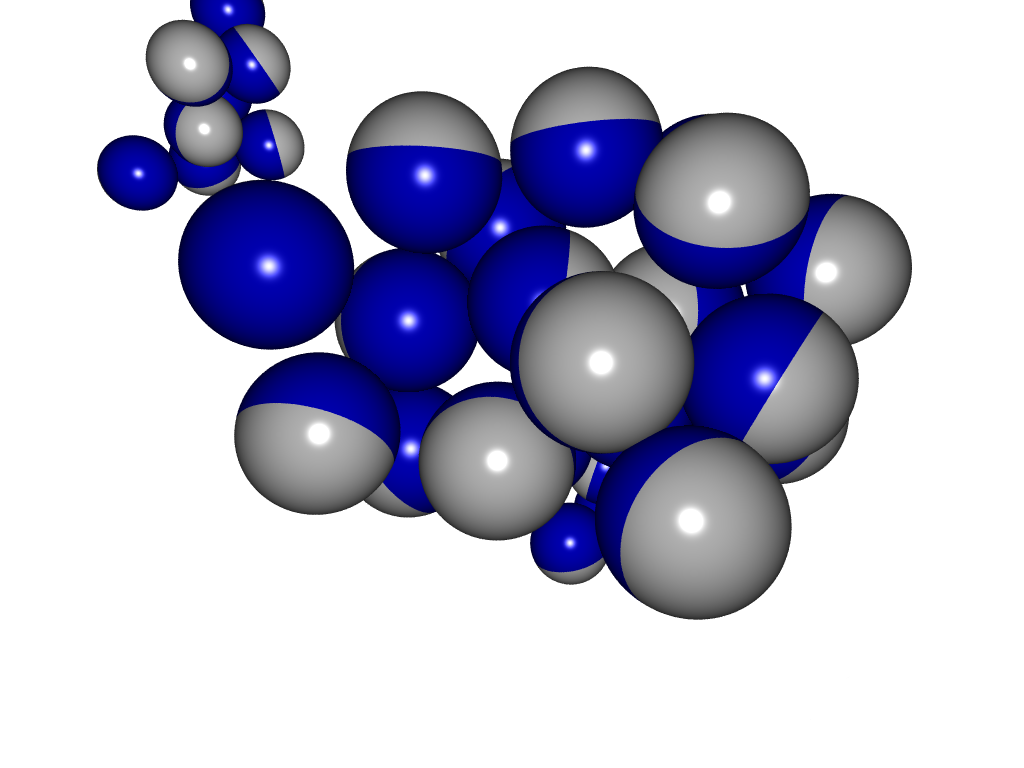
\includegraphics[width=0.45\textwidth]{janus/shotc}\label{fig:shotc}
	}

	\subfloat[]{
		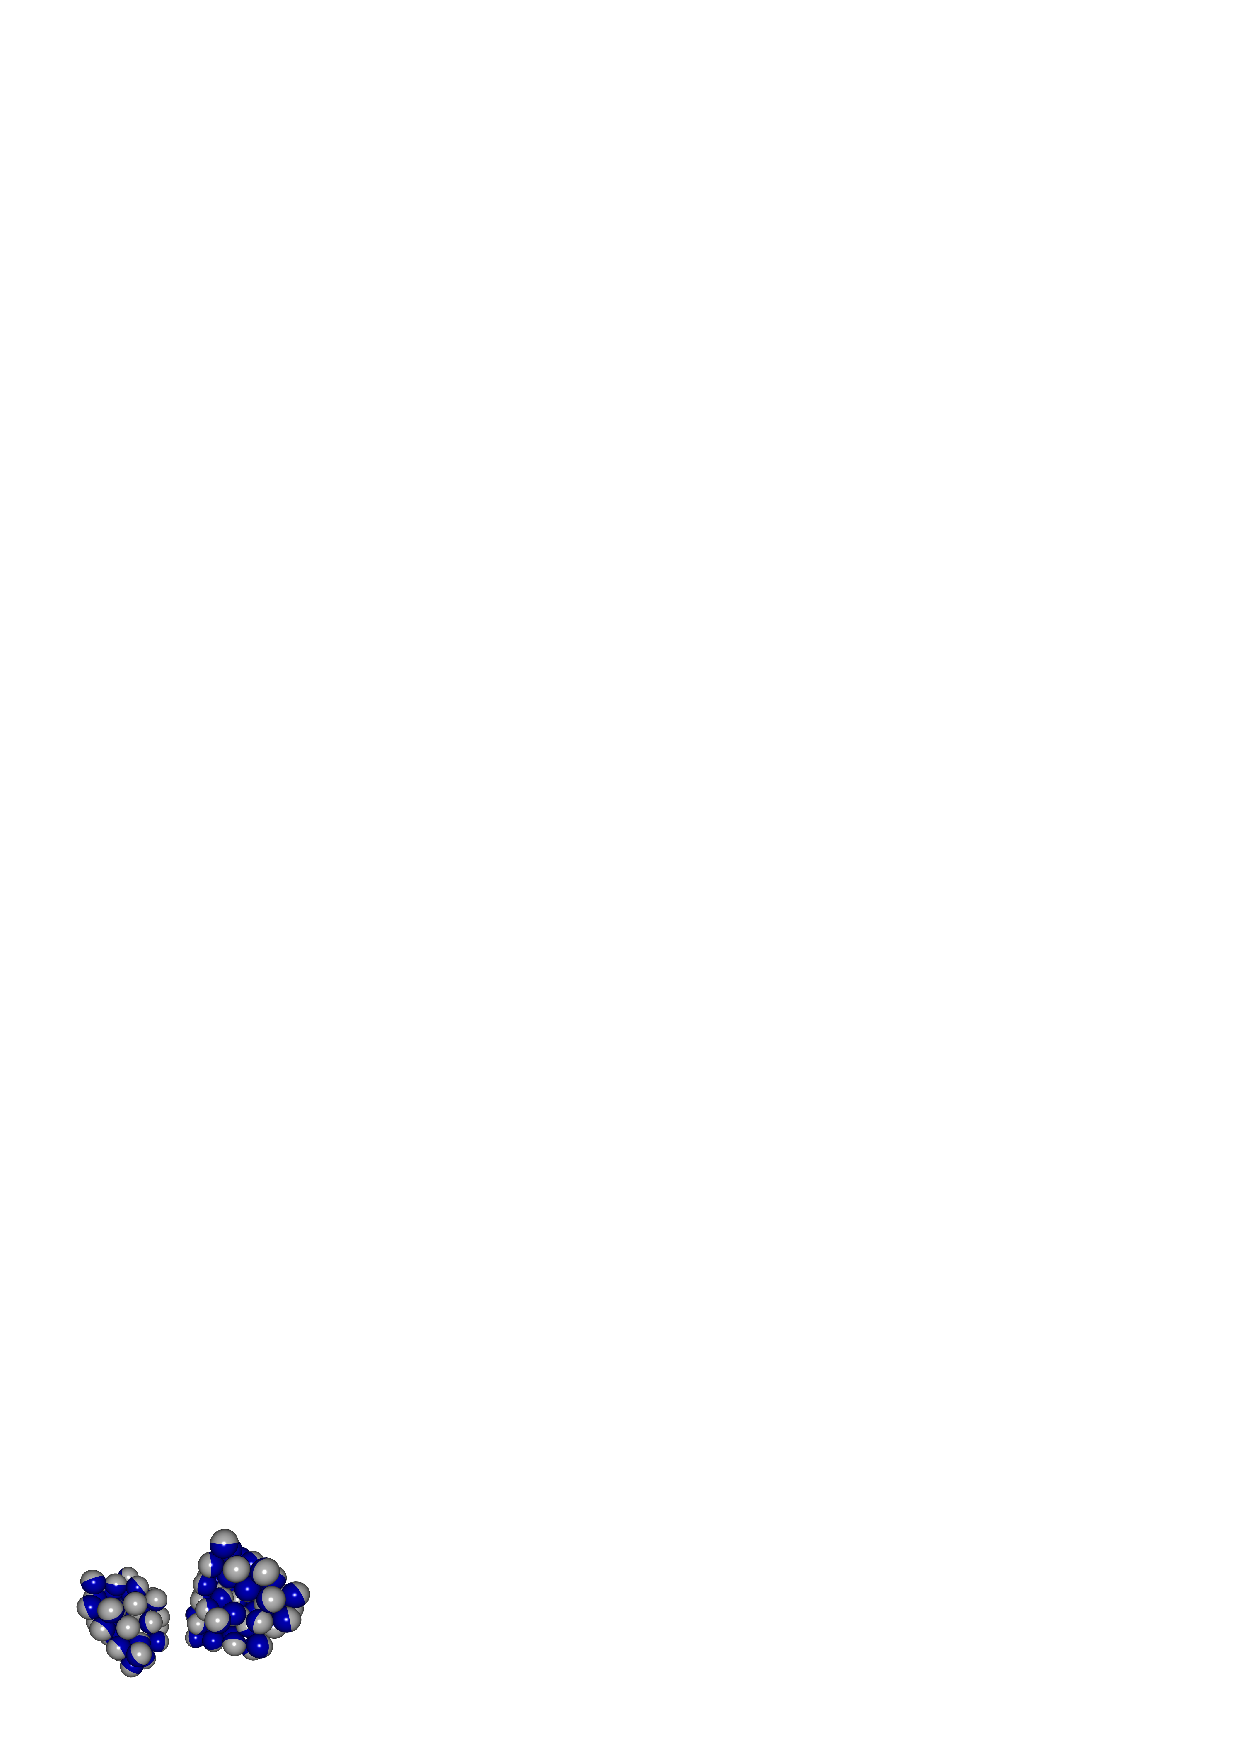
\includegraphics[width=0.45\textwidth]{janus/shot1}\label{fig:shot1}
	}
	\subfloat[]{
		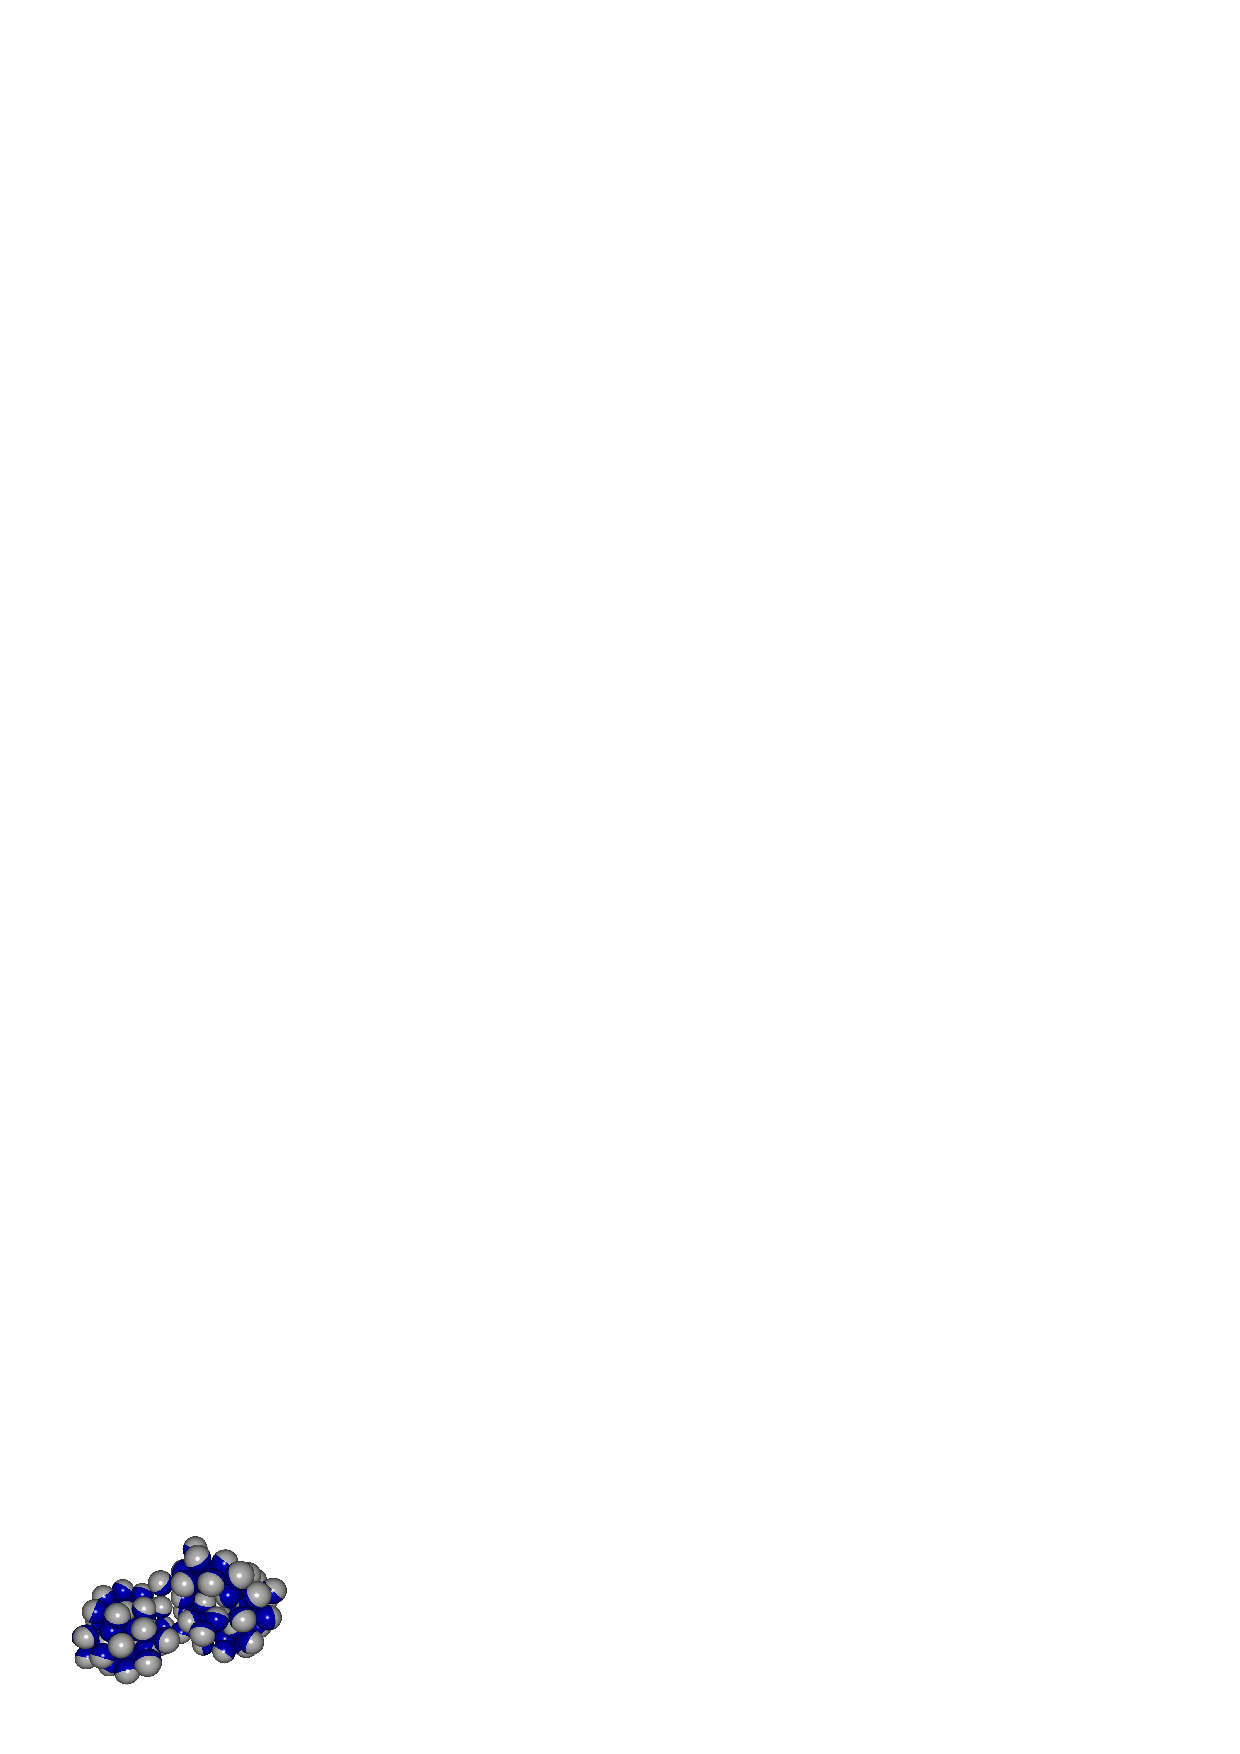
\includegraphics[width=0.45\textwidth]{janus/shot2}\label{fig:shot2}
	}	

	\subfloat[]{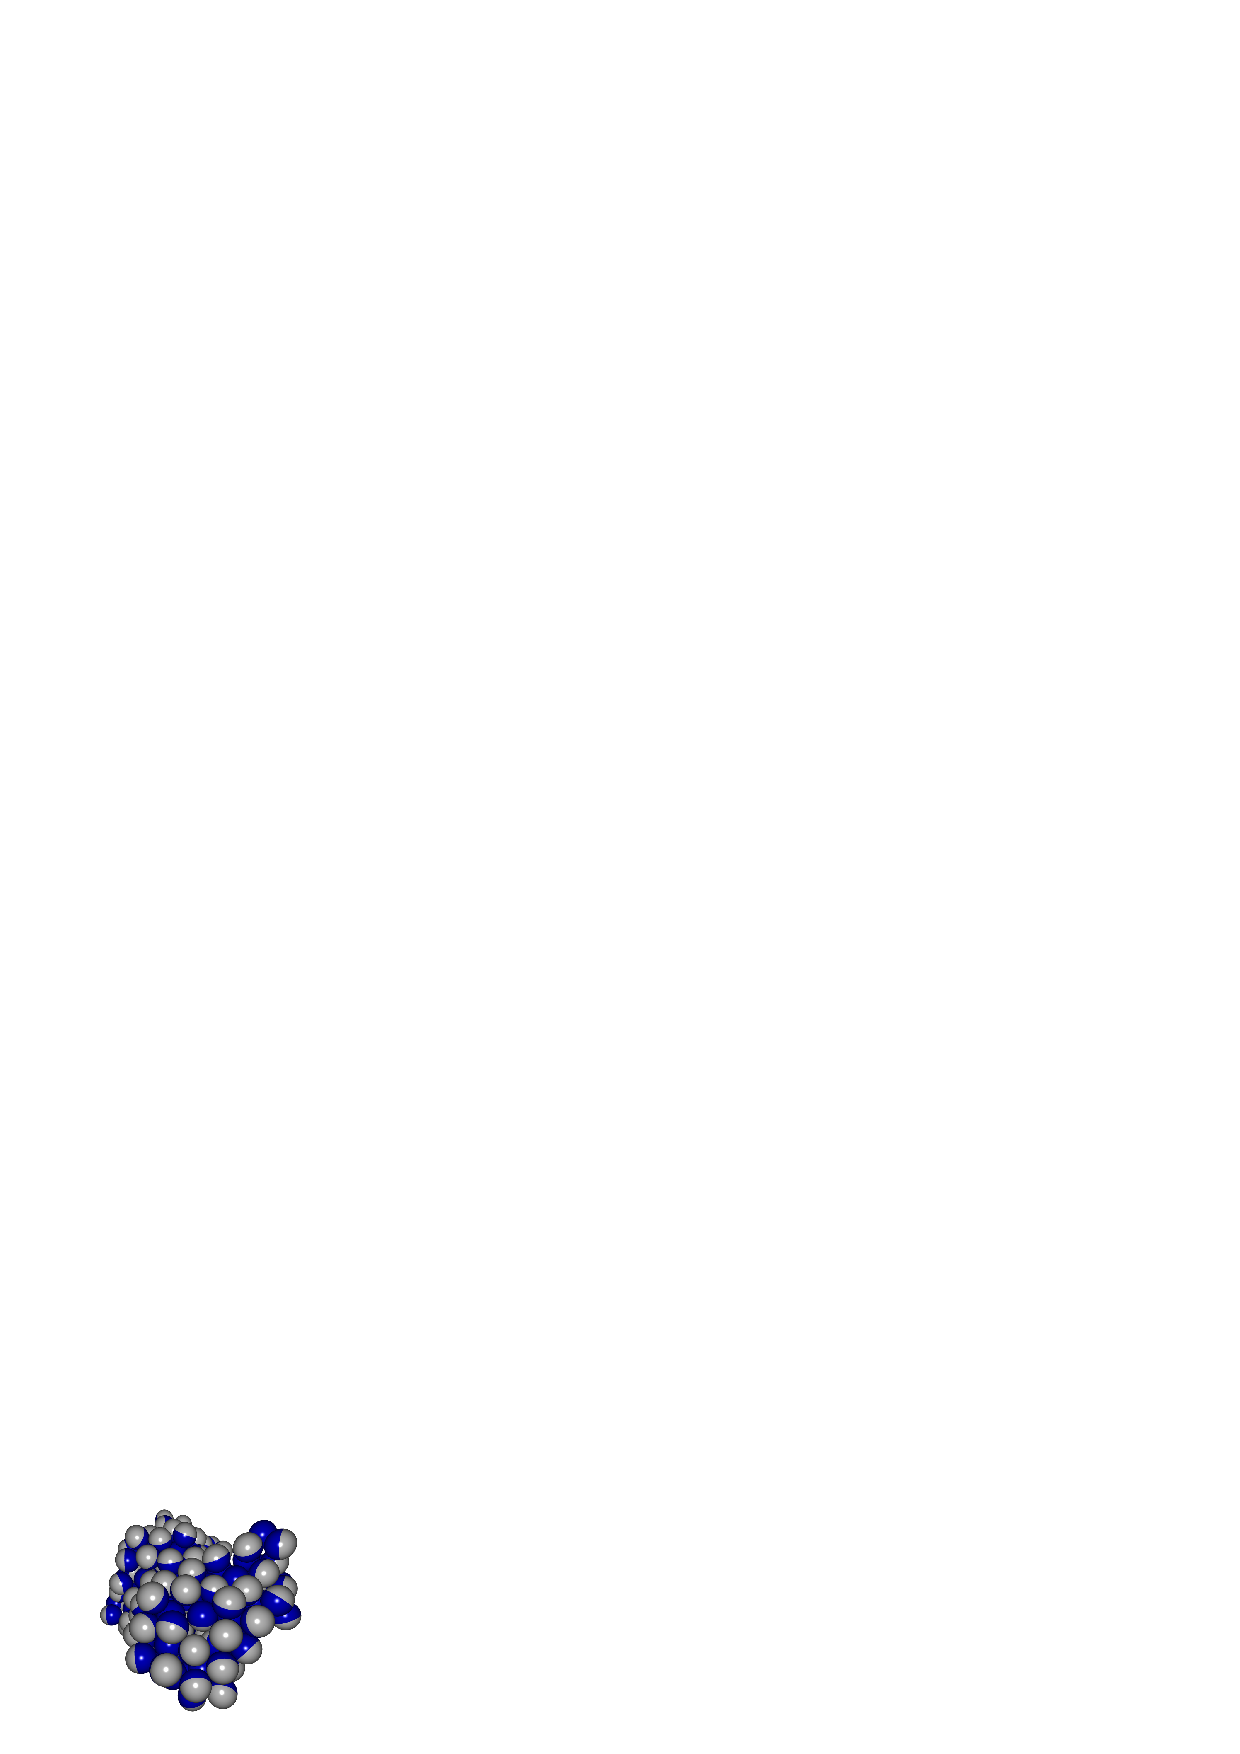
\includegraphics[width=0.45\textwidth]{janus/shot5}\label{fig:shot5}
	}
	\subfloat[]{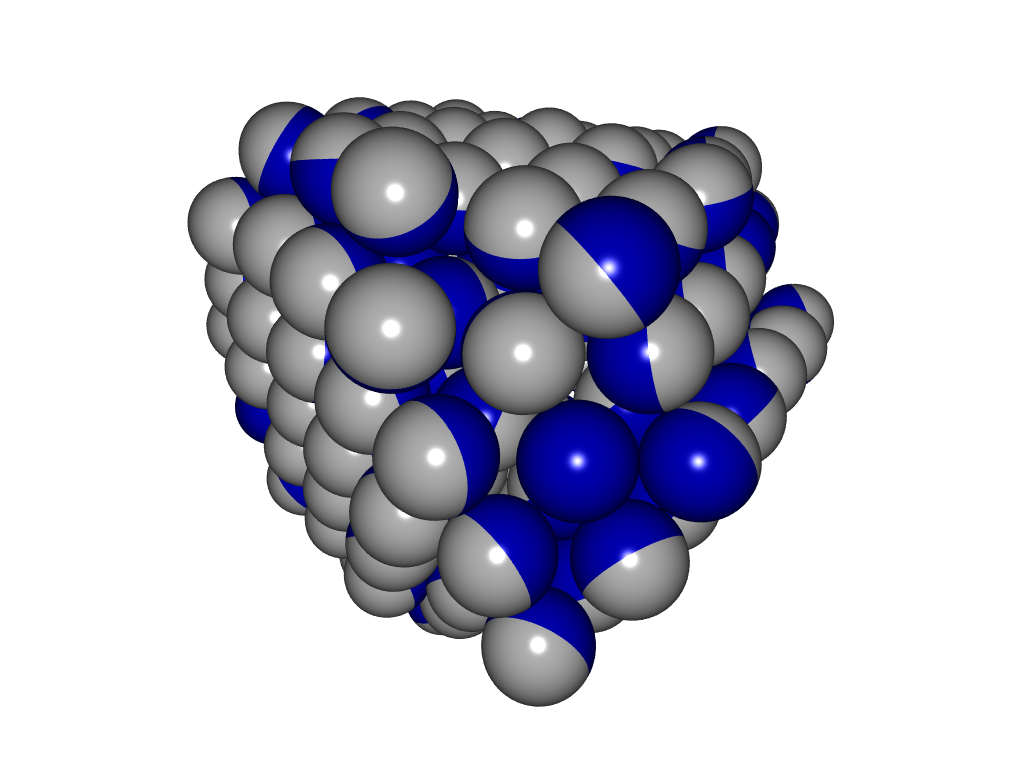
\includegraphics[width=0.45\textwidth]{janus/shot6}\label{fig:shot6}
	}\end{center}
	\caption[Snapshots of cage formation]{Sequence of six snapshots (\subref{fig:shota}$\rightarrow$\subref{fig:shot6}) from our simulations showing faceted cage formation
	via fast folding of short worm-like clusters (\subref{fig:shota}-\subref{fig:shotc}) and subsequent fusion of fluid blobs (\subref{fig:shot1}-\subref{fig:shot6}).}\label{fig:snapshots}
\end{figure}

A statistical analysis of our data correlating  size and structure for non-planar aggregates in region~\subref{fig:patch105} indicates a clear preference for large clusters to develop into  faceted hollow cages (see Figure~\ref{fig:facetvsnon}). 
What sets the onset cluster size for this transformation is a complex compromise between the geometric constraints imposed by the interparticle potential; the energy gain to close-pack particles in a bilayer, which grows with the number of particles $N$; the energy cost for sides and corners, which have on average fewer neighbors than in a fluid state and have an energy cost which grows as $ N^{1/2}$ and $N^{0}$, respectively; and finally the entropy loss due to particle ordering.
Clearly, as $N$ increases, at sufficiently large binding energy, planar configurations become the most stable, and this results in surface faceting.

\begin{figure}
	\begin{center}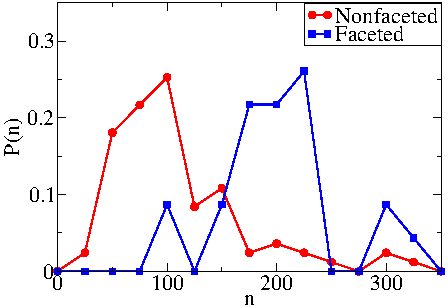
\includegraphics[width=0.6\textwidth]{janus/facetvsnon}\end{center}
	\caption[Probability distribution function of cluster size]{Probability distribution function $P(n)$ as a function of cluster size $n$ for fluid and faceted aggregates
	in region~\subref{fig:patch105} of the phase diagram.}\label{fig:facetvsnon}
\end{figure}

When $\theta_{\rm max}$ increases to even larger values, the geometric constraints imposed by the interparticle potential become less restrictive, and  planar bilayer configurations
become less stable. 
Phase~\subref{fig:patch110} is characterized by fluid, amorphous blobs which remain fluid at all sizes. 
Large clusters, formed by the smooth fusion of smaller ones, tend to contain smaller sub-clusters in their interior. 
This is the first sign indicating that aggregates begin to acquire a three-dimensional character, which eventually leads to the formation of clusters with fcc  order, as inner and outer clusters begin to interact with each other.

The location of the fluid to fcc transition is at $\theta_{\rm max}\simeq 135^{\circ}$, and was found by performing a structural analysis of the aggregates. 
Using the order parameters defined in Section~\ref{sec:orderparamdesc}, we measure the degree of crystallinity of the self-assembled aggregates.
\comment{
	Following~\cite{auer,tenwolde}, we identified particles whose local orientation is compatible to fcc ordering via a local bond order parameter based on spherical harmonics.
Given a particle  $i$, we consider
	\begin{equation}
		Q_{6m}(i)=  \frac{1}{N_b(i)}    \sum_{j=1}^{N_b(i)} Y_{6m}({\bf r}_{ij})\,,
	\end{equation}
where $j$ runs over the $N_b(i)$ neighbors of  particle $i$, from which a rotationally invariant order parameter correlating the orientation of neighboring particles $i$ and $j$ can be defined as
	\begin{equation}
		{\bf q}_6(i)\cdot {\bf q}_6(j)= \sum_{m=-6}^6 Q_{6m}(i) \cdot Q^*_{6m}(j)
	\end{equation}\label{orderparamdesc}
}
Figure~\ref{fig:q6q6} shows the degree of crystallinity $\left<O\right>$ as a function of  $\theta_{\rm max}$ across the angular range $\theta_{\rm max}\in[120:180]$.
$\left<O\right>$ is obtained by first averaging ${\bf q}_6(i)\cdot {\bf q}_6(j)$ over the neighbors of each particle $i$, and then by taking the average over all crystalline particles in a cluster. 
Clearly, once crystalline particles are formed, their degree of order in a fcc crystal structure is independent of $\theta_{\rm max}$.
\begin{figure}
	\begin{center}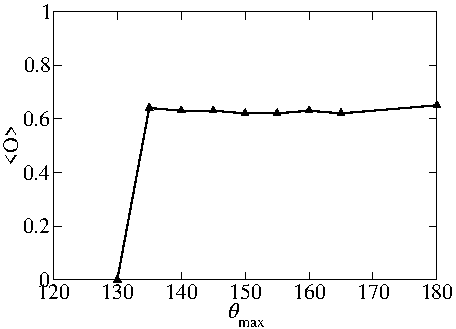
\includegraphics[width=0.6\textwidth]{janus/q6q6}\end{center}
	\caption[Degree of crystallinity of aggregates vs. hydrophobic area]{Degree of crystallinity of self-assembled aggregates as a function of hydrophobic area $\theta_{\rm max}$.}
	\label{fig:q6q6}
\end{figure}

The explanation of this behavior is purely geometrical.
In fact, for sufficiently large $\theta_{\rm max}$, the hydrophilic area on each particle becomes so small that can be positioned among the 12 particles' contact points resulting from an fcc crystal without affecting its structure.
Simple geometric considerations suggest that the onset value should occur for an angular span on the order of $150^{\circ}$.
This value is compatible with our result $\theta_{\rm max}\simeq 135^{\circ}$, especially considering the extra tail of $10^{\circ}$ in our definition of the potential angular dependence. A careful analysis of the model for decreasing values of $\theta_{\rm tail}$, not shown here, does indeed result in a systematic shift of the crystallization onset $\theta_{\rm max}$ to larger values.

\begin{figure}
	\begin{center}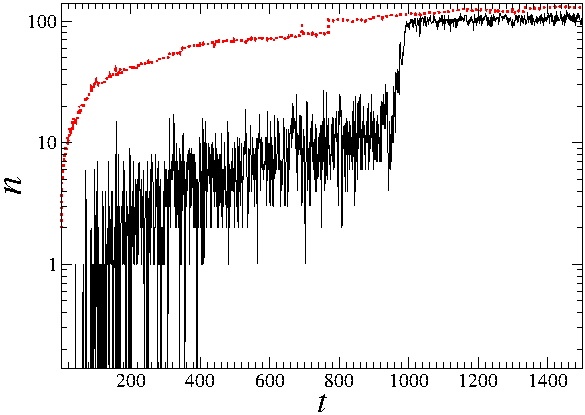
\includegraphics[width=0.8\textwidth]{janus/nucleation}\end{center}
	\caption[Aggregate size vs. time for $\theta_{\rm max}=160^{\circ}$]{\label{fig:nucleation} Linear-Log plot of the typical aggregate size $n$ as a function of time. The dotted line shows the total number of particles in the aggregate, while the continuous line shows how many of those particles are tagged as crystal-like. These data were collected at $\theta_{\rm max}=160^{\circ}$.}
\end{figure}

Finally, it is important to point out that, once again, the pathway leading to the formation of crystalline aggregates occurs in a two-step fashion.
Particles first condense into a large, fluid aggregate, and then crystallize from within the cluster via a standard nucleation process.
Figure~\ref{fig:nucleation} shows in the same plot the aggregate size and the number of crystalline particles in the aggregate versus time for a system with $\theta_{\textrm{max}} = 160^{\circ}$.
Clearly, crystal formation begins long after the aggregate is formed, and the large fluctuations in the initial stages of crystal growth show the typical signature of crystal nucleation. 
These results are compatible with nucleation studies of isotropic colloidal particles interacting via a short-range attractive potential first observed in~\cite{tenwolde}, and highlight the crucial role played by metastable phases in the dynamics of crystal growth.
In fact, we believe that this is the overarching physics behind the rich dynamical phenomenology we find throughout this paper. 

Self-assembly proceeds, as predicted by Ostwald's step rule in the context of crystal nucleation~\cite{ostwald}, in a stepwise fashion that accounts for the  complex free energy landscape containing  multiple metastable states.
Ostwald's step rule states that, as a general rule, when multiple crystalline phases are possible, it is not the most, but the least stable form which crystallizes first -- equilibration may then proceed in steps to the most stable configuration.

Although we have not looked at the stability of the different phases found in our simulations, planar and vesicular structures are also observed in the study of the equilibrium properties of a model system similar to ours~\cite{SciortinoX}.
It is also worth mentioning that we expect the precise location of the phase boundaries to be somewhat sensitive to the particular choice of the angular potential. 
Unfortunately, this is very hard to characterize experimentally near the Janus interface and there is not a unique way of modeling that boundary.
Our phase diagram is therefore intended to serve mostly as a guide for experimentalists, and not to model any specific category of amphiphilic particle.

\section{Conclusions}
In this chapter we used molecular dynamics simulations to study the self-assembly pathways of spherical  amphiphilic colloidal particles.
We uncovered a wealth of different aggregates whose structures  span the three-dimensional spectrum.
Specifically, depending on the size ratio between the hydrophilic and  hydrophobic regions, particles self-assemble into small micellar clusters, worm-like structures, planar bilayers, faceted and fluid cages, and finally fcc crystals.
We described  the hierarchical self-assembly pathway leading to most of these structures and discussed their connection to the geometry of local interparticle interactions.
Finally, we made precise predictions  for the formation of hollow amphiphilic cages.

Although the morphology  of some of our aggregates can be predicted by simple geometric considerations, the dynamics leading to their formation is far less trivial, and may play a crucial role in the efficiency of the self-assembly process.
We believe that, apart from trivial cases, any procedure attempting to design interparticle interactions to target specific structures could greatly benefit from taking into account the dynamics of structure formation in the design process.


%\part{Crystallization of Hard Aspherical Particles}
%\label{sec:corpus}
%\chapter{Phase Behavior of Hard Aspherical Particles}
\chapter{Phase behavior of hard aspherical particles}
\label{chap:aspherical}

\section{Introduction}
Problems of packing and space tiling have fascinated scientists for a very long time.
Kepler's 1611 essay {\it ``Strena Seu de Die Nive Sexangula''} (``A New Year's Gift of Hexagonal Snow'')~\cite{Kepler} is probably one of the earliest publications on the subject.
Herein he conjectured that cubic close packing and hexagonal close packing are the most efficient ways to fill a space using equally sized spheres.
It wasn't until 1998 that Kepler's conjecture was finally announced to be proven (with a 99\% degree of confidence) by Thomas Hales~\cite{Hales}.

Most of the work on particle crystallization and self-assembly in the last decade has focused on monodisperse~\cite{frenkel1} or polydisperse~\cite{frenkel2,zaccarelli} systems of spherical or regularly-shaped particles (see also~\cite{glotzer,chandler,geissler,cacciuto,torquato,frenkel,glotzer2,glotzer3,glotzer4,esco,weitz} and references therein).
Nevertheless, there are several important cases in which the shape of the single components cannot be tailored at will; however, an efficient packing, or an understanding of the physical properties of these densely compressed systems, is highly desirable.
Two examples of outstanding problems in this category are the storage of grains~\cite{deGennes} and protein crystallization~\cite{rosenberger}.
Both examples can be ideally thought of as two different aspects of the problem of understanding the role of shape in particle packing.
In the first case the goal is to efficiently pack a system of randomly-shaped polydisperse grains; 
in the second, the aim is to crystallize non-spherical, yet equally shaped monodisperse components. 
In this chapter, both of these cases will be addressed. 

An understanding of the relationship between the ability of particles to form macroscopically-ordered crystal structures and their shape is sought.
Specifically, we analyze how random perturbations from the ideal spherical shape affect the crystallizability of a densely packed system of indistinguishable hard particles.
Although a few papers have  dealt with the thermodynamic behavior of soft/deformable particles as a model for polymer brushes or polymer-coated colloids (\cite{pamies,capone,richter,bozorgui} and references therein), this is the first study where shape distortions, frozen onto the particles, are explicitly and systematically accounted for.

Crystallization in these systems occurs because of the free volume gain associated with the crystal structure, as discussed in Section~\ref{sec:CNT}.
However, even in simple systems, precise calculations of the free energies involved in these transitions are very difficult. 
In complicated systems such as those discussed in this chapter, it is implausible to perform these calculations rigorously, and since the transition depends on small differences between large free energy values, computer simulations are the tool of choice to study and analyze this important process in detail.

\comment{The problem of crystal formation is poorly understood.
From a thermodynamic standpoint, classical nucleation theory informs us that a crystal can only be formed via a barrier crossing event.
The free energy gain to form a nucleus of a stable crystalline structure in a supersaturated solution must balance out the free energy cost associated with the formation of an interface between the solid and the fluid parent phase.
The Gibbs free energy cost, $\Delta G$, associated with this event has a strong dependence on the interfacial free energy, $\gamma$: ${\Delta}G \propto \frac{\gamma^3}{(\rho\Delta\mu)^2}$,  where $\rho$ and $\Delta\mu$ are the density and the chemical potential difference between solid and fluid phase, respectively.
As $\gamma$ is very hard to extract from experiments, computer simulations are the tool of choice to study and analyze this important process in detail.}

\section{A model of hard aspherical particles}\label{sec:asphermethod}
In this chapter, each particle is built by randomly setting the center of $N_b$ ($4 \leq N_b \leq 12$) spheres of diameter $\sigma$ inside a spherical shell of diameter  $\sigma_0<\sigma$.
The overall volume generated from the resulting overlapping aggregate defines our new particle.

Deviations from the ideal spherical shape can be conveniently controlled by varying $\sigma_0$ and $N_b$. 
For  $\sigma_0=0$ one recovers the spherical limit, and as  $\sigma_0$ increases, particles develop larger and larger shape distortions.
In a similar fashion, large values of $N_b$ result in a bumpy but overall isotropic particle, whereas small values of $N_b$ tend to generate very anisotropic shapes.

Once a particle is built, the center of mass of this cluster of balls is determined, and the entire cluster is scaled so that its total volume equals that of a spherical particle of diameter $\sigma$, i.e. $\frac{\pi}{6}\sigma^3$.
Any two particles $i$ and $j$ interact via a hard repulsive potential defined as
\begin{equation}
U_{ij}=
\begin{cases}
0 & {\textrm{if }} |r_s-r_t|>\sigma_R \,\,\,\,\,\,\forall s\in i \,\,,\,\, \forall t\in j \cr
\infty &\text{otherwise}\cr
\end{cases} \,,
\end{equation}
where $s$ and $t$ run over all spheres of rescaled diameter $\sigma_R$ constituting particle $i$ and particle $j$ respectively.
Experimental realizations of colloidal particles similar to ours could be generated using the approach described in~\cite{weitz} to create uniform nonspherical particles with tunable shapes.  

Figure~\ref{shapes} shows a few snapshots of particle shapes obtained for different values of $N_b$ and  $\sigma_0$.
In Section~\ref{sec:polydisperse}, a specific $N_b$ and $\sigma_0$ will be chosen and a system will be composed of different random particles generated using the method above with those two parameters as inputs; in Sections~\ref{sec:disorderpress} and~\ref{sec:disorderyesno}, a system will be made up of identical particles from one specific outcome of the particle generation procedure.
\begin{figure}
	\begin{center}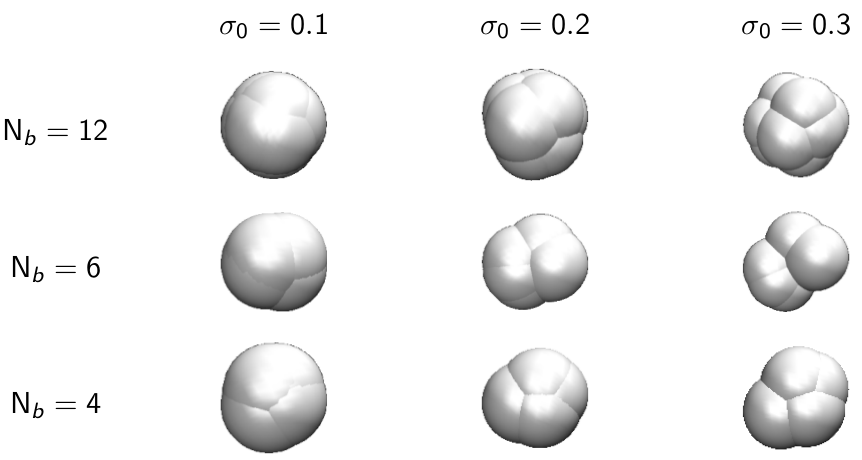
\includegraphics[width=0.8\textwidth]{disorder/parts2.png}\end{center}
	\caption[Model particles for different values of $\sigma_0$ and $N_b$]{Model particles for different values of $\sigma_0$ and $N_b$ built according to the scheme described in the text.}\label{shapes}
\end{figure}

Two order parameters characterizing the degree of asphericity of a particle are useful for relating the shape of particles in a system. 
The first is its asphericity, $A$ (as opposed to the commonly used sphericity, $S$~\cite{sphericity}), defined in terms of the surface to volume ratio of a particle $\alpha_p=\frac{A_p}{V_p}$ with respect to that of a sphere of diameter $\sigma$, $\alpha_s=\frac{6}{\sigma}$, as
\begin{equation}
	A = 1 - S = 1-\frac{\alpha_s}{\alpha_p} \,.
\end{equation}
Given our model setup, $V_p=V_s$, $A$ simplifies to 
\begin{equation}
	A=1-\frac{\pi\sigma^2}{A_p} \,.
\end{equation}

The surface area of a particle, $A_p$, is calculated via a simple Monte Carlo algorithm: a random point on the surface of a random one of the $N_b$ spheres is chosen, and it is determined whether it is inside any of the other spheres or not -- only points which do not lie on the inside of any other sphere are on the surface of the overall particle.
This is repeated until the proportion of points on the surface of the particle as a fraction of all points chosen converges; using this fraction and the total surface area of all of the spheres combined, $N_b \times \pi \sigma_R^2$, the surface area of the particle can be calculated.
 
The second parameter, $q$, measures the orientational symmetry  of the particle.
It is used to describe the  asphericity of random walks~\cite{rudnick}, and it is obtained by combining invariants of the particle inertia tensor $I_{ij}$  as
\begin{equation}
	q=\frac{\left(R_1^2-R_2^2\right)^2 + \left(R_1^2-R_3^2\right)^2 + \left(R_2^2-R_3^2\right)^2}{2\left(R_1^2 + R_2^2 + R_3^2\right)} \,,
\end{equation}
where $R_1$, $R_2$, and $R_3$ are the three principal eigenvalues of the inertia tensor of the particle, that is, the three principle radii of gyration of the particle.

Both parameters are defined so that they are equal to $0$ for a perfectly spherical particle, and approach $1$ for  extremely aspherical ones. 
Note that $A$ depends intimately on the value of $\sigma_0$ used to construct the particle, whereas $q$ depends only on the angular distribution of spheres about the center of mass -- that is, it is completely independent of $\sigma_0$.

It is worth briefly describing the limits of $q$, in particular, as its definition is less intuitive than that of $A$.
As defined, the $q \rightarrow 0$ limit is a sphere; $q \simeq \frac{1}{2}$ for a thin, circular plate; and $q \rightarrow 1$ for a long, thin rod.

\section{Shape-polydisperse systems}
\label{sec:polydisperse}
\comment{\subsection{Introduction}

Understanding how objects pack or can be designed to tile the three dimensional space is a fundamental optimization problem that has important practical applications that
range from the macroscopic, such as the efficient storage of grains,  to the microscopic: the fabrication of band-gap photonic materials.
Mathematicians have been intrigued by such problems for centuries; namely since Kepler's 1611 essay {\it On the Six-cornered Snowflakes}, but it wasn't 
until recently, with the advent of nanotechnology and the explosion of molecular biology, that problems of packing and self-assembly of nanoscopic components 
gained   tremendous traction in the broader scientific community.   
Recent advances in synthesis of nanoparticles~\cite{DeVries,Schnablegger,Hong,Weller,Hobbie,weitz,pine,mitragotri} allowed for unprecedented control over the 
 shape and surface chemistry of colloidal particles, thus providing an unlimited number of building blocks whose 
 spontaneous aggregation could lead to the formation of an unprecedented variety of structures with potentially novel functional, mechanical, and optical properties.
 Unlike most of the work on particle crystallization and self-assembly that in the last decade has focused on 
 monodisperse~\cite{frenkel1} or polydisperse~\cite{frenkel2,zaccarelli} systems of spherical or regularly-shaped particles  (see also~\cite{glotzer,chandler,geissler,cacciuto,torquato,frenkel,glotzer2,glotzer3,glotzer4,esco,weitz} and references therein), surprisingly little or nothing has been done
 theoretically to understand the packing of irregularly shaped particles. 
Indeed, there are several important cases in which the shape of the single components cannot be tailored at will,
 yet, an efficient packing, or an understanding of the physical properties of these densely compressed systems, is highly desirable.
Two examples of outstanding problems in this category are the storage of grains~\cite{deGennes} and protein crystallization~\cite{rosenberger}.
Both examples can be ideally thought of as two different aspects of the problem of understanding the role of shape in particle packing: systems of either polydisperse or indentically-shaped (monodisperse) components. 
  
Here we seek to gain insight into the crystallization of nonspherical particles. 
 We want to understand how  particle geometric features can be related to their ability to orderly pack into three dimensional periodic structures,
 and especially  to identify under what conditions they cease to do so. 
 We have recently reported~\cite{disorder1}  that it is possible to empirically relate particle geometry to crystallizability (intended as the tendency of a component to crystallize) 
by using two simple geometric parameters. The first is the particle asphericity  $A$, defined in terms of the 
surface to volume ratio of a particle $\alpha_p=A_p/V_p$ with respect to that of a sphere of diameter $\sigma$, $\alpha_s=6/\sigma$, as
$A =1-\alpha_s/\alpha_p.$  The second parameter, $q$, is related to the  orientational symmetry  of the particle.
It is used to describe the  asphericity of random walks~\cite{rudnick}, and it is obtained by combining invariants of the particle inertia tensor $I_{ij}$  as
$q=\sum_{i< j} (\lambda_i^2-\lambda_j^2)^2/\sum_i \lambda_i^2$, where $\lambda_i$, with $i=1, 2, 3$, is an eigenvalue of $I_{ij}$.
 
In this paper we try to rationalize those empirical results by computing how random perturbations from the ideal spherical 
shape affect the fluid-solid coexistence pressure of  monodisperse and shape-polydisperse systems of hard aspherical particles.

In order to generate a  statistical ensemble of aspherical particles, we developed a simple model~\cite{disorder1} that guarantees a certain degree of control over
the particle shape. Each particle is built by setting the center of $N_b$ ($4 \leq N_b \leq 12$) spheres of diameter $\sigma$ at random 
positions on the surface a spherical shell of diameter $\sigma_0<\sigma$.
The overall volume generated from the resulting overlapping aggregate defines our new particle.
Polydisperse systems of such aspherical particles were generated by choosing specific values of $N_b$ and $\sigma_0$ and allowing each particle in the system to arise from a different random collection of sphere positions.
Deviations from the ideal spherical shape can be conveniently controlled by varying $\sigma_0$ and $N_b$.
For  $\sigma_0=0$ one recovers the spherical limit, and as  $\sigma_0$ increases, particles develop larger and larger shape distortions.
In a similar fashion, large values of $N_b$ result in a bumpy but overall isotropic particle, whereas small values of $N_b$ tend to generate very anisotropic shapes.
Once a particle is built, the entire cluster is scaled so that its total volume equals that of a spherical particle of diameter $\sigma$, i.e. $\frac{\pi}{6}\sigma^3$.
Any two particles $i$ and $j$ interact via a hard repulsive potential defined as
\begin{equation}
U_{ij}=
	\begin{cases}
		0 & {\textrm{if }} |r_s-r_t|>\sigma_R \,\,\,\,\,\,\forall s\in i \,\,,\,\, \forall t\in j \cr
		\infty &\text{otherwise}\cr
	\end{cases}
\end{equation}
where $s$ and $t$ run over all spheres of rescaled diameter $\sigma_R$ constituting particle $i$ and particle $j$ respectively.
Experimental realizations of colloidal particles similar to ours could be generated using the approach described in reference~\cite{weitz,pine,mitragotri} 
to create nonspherical particles with tunable shapes. }

The results of simulations of polydisperse systems will be presented first.
Such systems could represent, for example, a system of colloidal particle which is ``sloppily'' synthesized with some tolerance for deviation from a perfect sphere.
Polydisperse systems have one major advantage, for a study such as that described below, over monodisperse systems: statistics.

In order to build up the statistical basis necessary to relate order parameters such as those described in Section~\ref{sec:asphermethod}, a large number of systems must be simulated for each data point; this severely limits the computational cost that may be expended per system.
Polydisperse systems represent a huge decrease in the number of independent variables; because each system is made up of a large number of different particle shapes, one may be confident that the result obtained is not a result of some peculiarity of a specific shape studied.
In Sections~\ref{sec:disorderpress} and~\ref{sec:disorderyesno}, monodisperse systems are studied, both as a comparison with the results attained in this section as well as using less computationally-intensive methods in order to study a larger number of particle shapes.

In order to determine the fluid-solid coexistence pressures for systems of aspherical particle, the method of direct fluid-solid coexistence simulation described in~\cite{noya} was used.
1024 particles were placed in an fcc crystal lattice (at volume density $\rho_s \simeq 0.545$, the hard sphere crystal coexistence density~\cite{HScoex}) centered in a box of dimensions $L_x \times L_y \times L_z$.
An fcc crystal was chosen based upon preliminary work, which indicated that when monodisperse aspherical systems form crystals, they tend to be (apart from a very few particular exceptions) fcc; no evidence has been found supporting the use of any other crystal geometry.

The dimensions of the box were chosen such that $L_x$ and $L_y$ were just large enough to accomodate the fcc crystal, and $L_z$ was roughly four times larger.
The crystal lattice was chosen such that the extension of the crystal in the $z$-direction was roughly twice that in the $x$- and $y$-directions, in order to increase the separation between the two fluid-solid interfaces in the system; by decreasing the surface-to-volume ratio of the crystal, one hopes to come as close to a ``bulk-like'' system as possible.

This crystal lattice was placed into equilibrium with a fluid of 1024 particles at hard sphere fluid coexistence volume density $\rho_l \simeq 0.495$.
The fluid and crystal were both briefly allowed to relax in order to relieve any overlap introduced by the ``bumpiness" of the particles and to allow the fluid to come fully into contact with the solid interface; because the particles are hard, there must be zero overlap in between particles.

Monte Carlo simulations were then run with constant number of particle $N$, pressure $p$, and temperature $T$ ($NPT$ ensemble), where the three box dimensions $L_x$, $L_y$, and $L_z$ were allowed to fluctuate independently under the isotropic pressure $p$.

The number of crystalline particles, $N_X$, in the system was monitored as a function of Monte Carlo step; this quantity was determined using the standard spherical-harmonics based bond order parameter $q_6$ described in Section~\ref{sec:orderparamdesc}.
Simulations were performed starting from a system initialized as desribed above, and $N_X$ was monitored over the course of the simulation to determine whether it decreased (crystal melting) or increased (crystal growth).

Below the coexistence pressure, the crystal will melt, and above it, the crystal will grow; thus, the pressure at which the system transitions (as a function of pressure) from decreasing $N_X$ to increasing $N_X$ represents the coexistence pressure $p^*$.
This method is known to have a few caveats: slow equilibration, non-negligible finite size effects,  dependence of the surface free energy on the specific face the crystal exposes to the fluid~\cite{noya}.
Nevertheless, for this specific system, we find this direct  method to be  more reliable than the two-step thermodynamic integration scheme described in~\cite{dijkstra}. 

\comment{\begin{figure}
	\begin{center}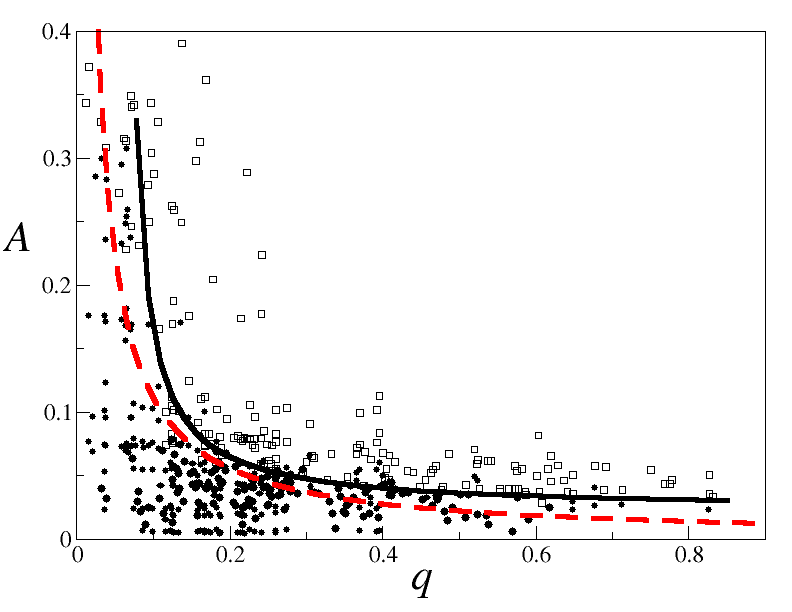
\includegraphics[width=0.8\textwidth]{polydisperse/mono1.png}\end{center}
	\caption[Crystallizability of monodispers aspherical particles vs. $A$ and $q$]{Crystallizability of monodisperse aspherical particles characterized in terms of two shape parameters $A$ and $q$. Filled circles indicate particles that easily crystallized, while open squares indicate particles that did not.  The dashed line represents a prediction of the crystallizability limit from the current work; see below.  Figure adapted from~\cite{disorder1}.}\label{mono1}
\end{figure}
Our empirical results on the crystallizability of   systems of monodisperse aspherical particles ~\cite{disorder1}, obtained by slowly compressing an ensemble of 487 different shape realizations
 are summarized in  Fig.~\ref{mono1} and indicate the existence of a clear boundary between particles that crystallize and particles that do not.
  A roughly inverse relationship is clearly evident; particles with large $A$ must have very small $q$ in order to have
a hope of crystallization, and vice-versa. This result provides a very useful way of predicting whether a particular particle shape can pack into a
crystalline structure by simply measuring the experimentally accessible $A$ and $q$. 
As this  model is intended to describe randomly shaped particles, the diagram does not include the results for particles designed with very specific shapes such as rods,
plates or regular polyhedral geometries that are known to crystallize. 
These particular cases would generate sharp peaks around specific values of $q$, and are purposefully excluded from this study.
 The solid line is  a guide to the eye and has the functional form $A(q) = 0.023 + 1/(170q-10)$.} 

Incorporating shape-polydispersity in these systems is not a trivial matter and requires some discussion.  
Unlike the common notion of polydispersity of spherical particles  for which any particle size can be indifferently used as a reference (and thus only the width, not the center, of the distribution matters), each particle shape could be used as a reference shape for this study. 
The problem is that the phase behavior could be very much dependent on the specific choice of $A$ and $q$.
We therefore adopted a pragmatic approach to describing shape-polydispersity  that has a natural experimental counterpart~\cite{weitz}. 

\begin{figure}
	\begin{center}
		\subfloat[]{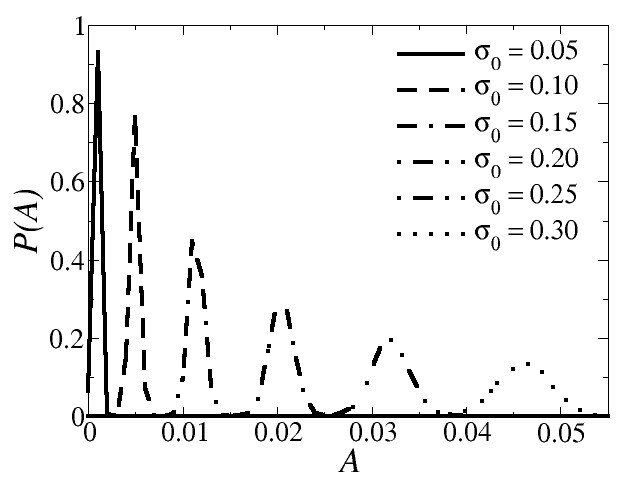
\includegraphics[width=0.6\textwidth]{polydisperse/Ahist.png}\label{Ahist}}

		\subfloat[]{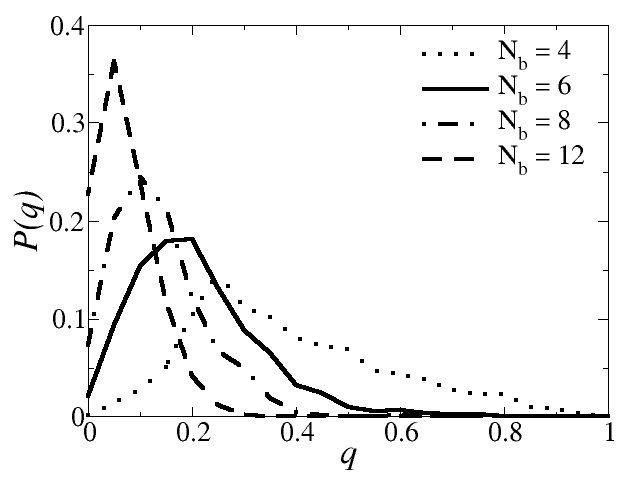
\includegraphics[width=0.6\textwidth]{polydisperse/qhist.png}\label{qhist}}
	\end{center}
	\caption[$A$ and $q$ distributions for different values of $\sigma_0$ and $N_b$]{\subref{Ahist} Probability distributions of $A$ for polydisperse systems with $N_b = 8$ and various values of $\sigma_0 \in [0.05,0.30]$.  the $A$ distribution is approximately independent of $N_b$.  \subref{qhist} Distribution of $q$ values for polydisperse systems with $N_b$ = $4$, $6$, $8$, and $12$.  Recall that $q$ is independent of $\sigma_0$.  The distribution is significantly larger and broader for $N_b = 4$ than for the larger values of $N_b$.}\label{histograms}
\end{figure}

Namely, we  consider the distributions of $q$s and $A$s arising when constructing our particle using a given number of spheres $N_b$ and a given value of $\sigma_0$.
Particles  with large values of $N_b$ generate narrow distributions shifted towards small values of $q$, while small values of $N_b$ ($N_b\geq 4$) result in wide distributions peaked over large values of $q$.
When $\sigma_0\rightarrow 0$ one recovers the  hard sphere limit for any value of $N_b$, and as $\sigma_0$ increases,  larger and larger values of $A$ will be sampled (without affecting the $q$ distributions) until approaching the crystallizability boundary.
Sample distributions of $A$ and $q$ for varying values of $\sigma_0$ and $N_b$ (respectively) are shown in Figure~\ref{histograms}

We systematically analyzed particles constructed with $N_b =4$, $5$, $6$, $8$, and $12$, and values of  $\sigma_0 \in[0.05,0.30]$.

\begin{figure}
	\begin{center}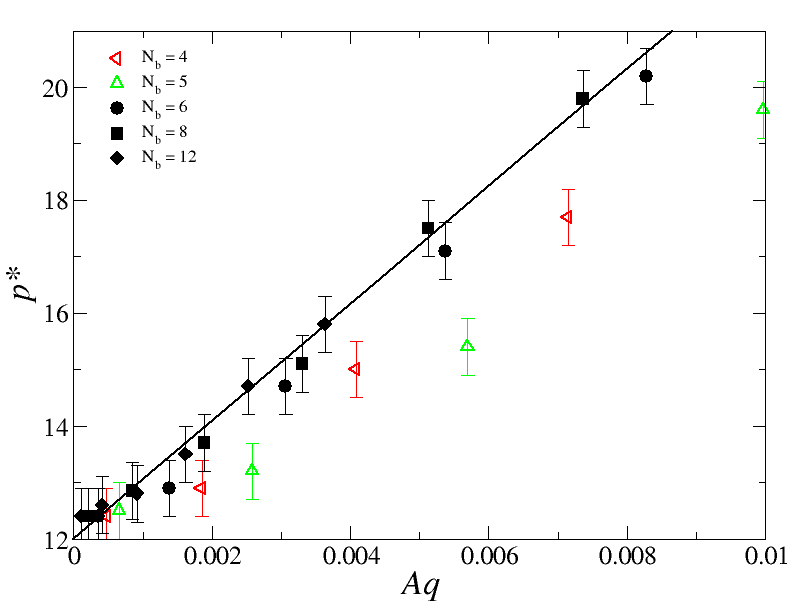
\includegraphics[width=0.8\textwidth]{polydisperse/poly.png}\end{center}
	\caption[Coexistence pressures for shape-polydisperse systems vs. $Aq$]{Coexistence pressure vs. $Aq$ for shape-polydisperse systems of hard aspherical particles. The solid line is a fit to the data for $N_b\geq 6$.}\label{poly}
\end{figure}
All data points have been computed using two different random sets of particle geometries from the given distribution.
The difference between the results from the two independent sets is smaller than the error bar associated with the numerical scheme.
Figure~\ref{poly} shows our results: the coexistence pressure $p^*$ (as defined above) versus the product $Aq$ for $4 \leq N_b \leq 12$ and $\sigma_0 \in [0.05,0.30]$.

Unsurprisingly, the coexistence pressure increases with increasing $A$ and $q$, but remarkably, for $N_b \geq 6$, the relationship between $p^*$ and $Aq$ is simple linear one.
We find that the coexistence pressures for these $N_b$ values  be fitted to  $p^* (A,q)= 991Aq + 12$.
Note that the y-intercept is near the hard sphere coexistence pressure of $p^*_{\rm HS}\simeq  11.7$~\cite{HScoex}, as it should be.
This should be expected because the $Aq \rightarrow 0$ limit is a system of hard spheres.

These results thus suggests that $p^*(A,q)$ can be expressed in terms of a Taylor expansion in the quantity $Aq$: 
\begin{equation}
	\frac{p^*(A,q)-p^*_{\rm HS}}{p^*_{\rm HS}} = \alpha Aq + ...
\end{equation}
Note, however, that significant but systematic deviations from the linear fit are visible for systems of particles obtained with  $N_b = 4$ and $N_b = 5$. 
These values of $N_b$ correspond to particles with  relatively large values of $q$ and rather broad distributions (see Figure~\ref{qhist}), suggesting that other, higher-order terms in the expansion may be necessary. 
Furthermore, for such wide distributions fractionation  between isotropic and anisotropic particles may become an important factor -- this is an effect to which the direct simulation method used here is completely blind, because the system is initialized with a preformed crystalline volume with a random selection of particles.
Fractionation would require complete melting of the initial crystal and subsequent formation of a fractionated crystal, which was not allowed in this study.

\section{Monodisperse systems: coexistence pressures}\label{sec:disorderpress}
\begin{figure}
	\begin{center}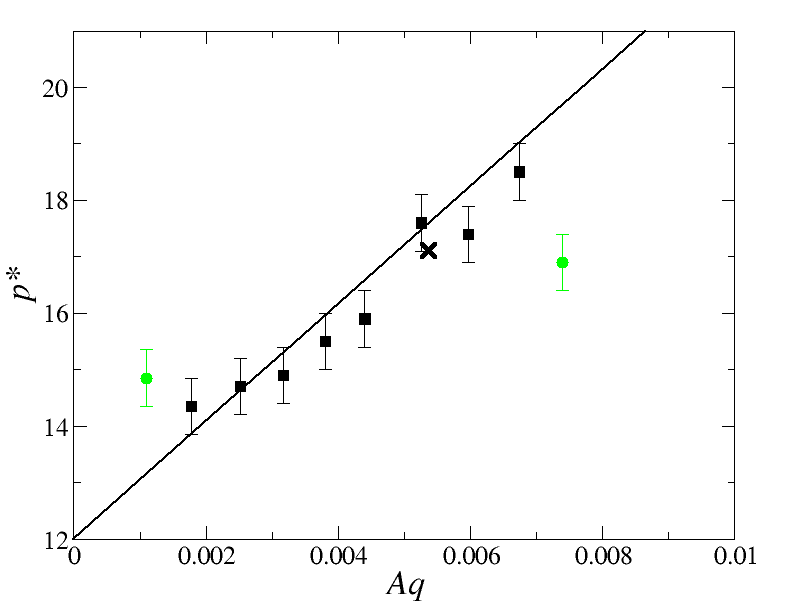
\includegraphics[width=0.8\textwidth]{polydisperse/mono2.png}\end{center}
	\caption[Coexistence pressure vs. $Aq$ for monodisperse systems of aspherical particles]{Coexistence pressure vs. $Aq$ for monodisperse systems of hard aspherical particles with $N_b = 6$, $\sigma_0 = 0.2$.  The line is a fit obtained from the data presented in Figure~\ref{poly} for polydisperse systems with $N_b = 6$, $8$, and $12$.  The cross indicates the position of the polydisperse system with $N_b = 6$, $\sigma_0 = 0.2$.
Points at the extremes of the $q$ distribution are shaded with a lighter color.}\label{mono2}
\end{figure}

The existence of a master curve for the coexistence pressure of significantly different particle distributions (provided $N_b\geq6$), both in terms of their average value  and their width, is quite remarkable, and provides a very compact and elegant way of expressing the equilibrium properties of such systems.  
As a test of the robustness of this relationship, ten monodisperse systems were generated by a single set of parameters: $N_b = 6$, $\sigma_0 = 0.2$.
Each of these systems is characterized, by definition, by an infinitely sharp $P(q)$, and individual configurations were selected to cover a fairly wide range of $Aq$ values, while keeping $A$ roughly constant (because the distribution of $A$ values for a given set $(N_b,\sigma_0)$ is narrow, see Figure~\ref{Ahist}). 
A plot of these data, shown in Figure~\ref{mono2}, indicates that the relationship adapted unaltered from the polydisperse case is a reasonably good predictor of coexistence pressure for the monodisperse case as well.
This is a clear indication that, up to some maximum, the master curve is overall independent of distribution width.

Notice that no coexistence pressures above $p^*(A,q) \simeq 21$ are reported. 
This is not a coincidence; in general, if a system was going to crystallize at all (that is, if the crystalline region of the simulation box was going to grow), the coexistence pressure $p^*$ was below this value.
This is interesting because this value is close to the fluid pressure of a system of hard spheres
at the glass transition density~\cite{speedy}, $p_G = 22.6$, and  it is reasonable to assume that $p_G$ sets an upper bound to the 
largest accessible fluid coexistence pressure for aspherical particles obtained with direct fluid/solid sampling.

In fact, this method  
is clearly susceptible to anomalies in system kinetics, thus making coexistence measurements at pressures larger than the ones herein reported 
quite cumbersome and somewhat unreliable. Nevertheless, if we assume that no aspherical hard particle will easily crystallize above $p_G$, we can 
formulate a prediction for whether a system of aspherical particles should be expected to easily crystallize: given $p^* \simeq 991 Aq + 12$, and based upon this simple line of reasoning, one should expect, as a first-order approximation, a limit of
\begin{equation}Aq \lesssim 0.011 \,.\label{xtallimit}\end{equation}
When the product $Aq$ is below this limit, the system would be expected to easily crystallize at some pressure; above the limit, the system is never expected to crystallize.

\section{Monodisperse systems: predicting crystallization}\label{sec:disorderyesno}

In order to test the prediction above, a large number of monodisperse systems was tested for the simple binary question: ``Does this system crystallize easily?''
In order to answer this question, traditional Monte Carlo simulations were performed in the $NPT$ ensemble.
Instead of intializing the system to be half crystalline and half fluid, a cubic box was used and the simulations was initialized in a fluid state.
Each simulation contained $N = 128$ particles and contained a monodisperse system of aspherical particles constructed with some value of $(N_b, \sigma_0)$; for the purposes of this study, we used $N_b \in \left\{4,6,8,12\right\}$ and $\sigma_0 \in \left(0,1\right)$.

The initial pressure was set to $p = 10$ and the pressure was incremented by $\Delta p = 0.5$ or smaller.
Each simulation was run for a minimum of $4 \cdot 10^6$ Monte Carlo sweeps after thermalization.
The simulation was ended when the system either crystallized or reached a volume fraction $\phi \simeq 0.6$, above the glass transition point of hard sphere, $\phi_G = 0.58$.
Crystallization was detected by a combination of (a) the $q_6$ order parameter, (b) a careful monitoring of the system volume fraction over time for sudden jumps (indicating a phase transition), and (c) visual inspection.
We investigated a total of $487$ different particle geometries. 

Figure~\ref{mono1} summarizes the result of this study. 
\begin{figure}
	\begin{center}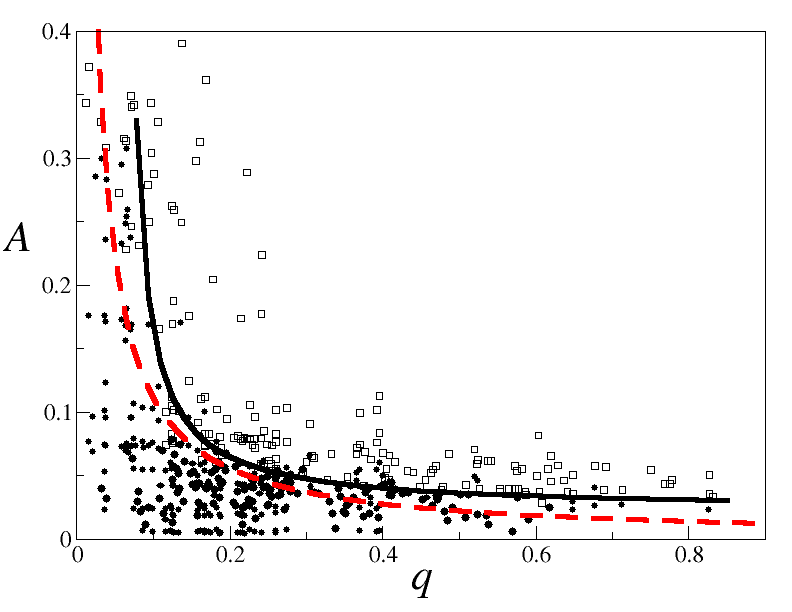
\includegraphics[width=0.8\textwidth]{polydisperse/mono1.png}\end{center}
	\caption[Crystallizability of monodisperse aspherical particles vs. $A$ and $q$]{Crystallizability of monodisperse aspherical particles characterized in terms of two shape parameters $A$ and $q$. Filled circles indicate particles that easily crystallized, while open squares indicate particles that did not.  The solid line is a guide to the eye constructed between the two distinct regions in which particles crystallize or not.  The dashed line represents a prediction of the crystallizability limit from above, $Aq = \simeq 0.011$.}\label{mono1}
\end{figure}
It is obtained by collecting 
the crystallizability of the 487 systems built out of the 487
different particle geometries we have generated across the $A$, $q$ spectrum. 
Each point in the $A$ vs $q$ diagram represents the result of a set of simulations at different pressures.
As would be expected, crystallization is favored when both $A$ and $q$ are small -- that is, 
when the particles are nearly spherical by both measures.  
A roughly inverse relationship is clearly evident; particles with large $A$ must have very small $q$ in order to have
a hope of crystallization, and vice-versa.
But more importantly, we find the existence of a clear boundary delineating the crystallizability limit 
for every possible shape generated with our model (small deviations at the interface are
likely due to finite size effects and/or the limited length of our simulations).

This is quite remarkable because it provides a very useful way of predicting whether a particular particle shape can pack into a
crystalline structure by simply measuring the experimentally accessible $A$ and $q$. 

Notice that for smaller values of $q$ our data seem to 
indicate a sharp end of the crystal boundary. We believe this to be an artifact of our particle model.
In fact, that region is where the value of $\sigma_0$ becomes sufficiently  large ($\sigma_0>0.5\sigma$)
to break the compactness of the particles generated with our method, especially those with smaller values of $N_b$. 
Furthermore, as small values of $q$ indicate a large orientational symmetry, we expect this
region to be heavily populated by specific  geometric arrangements (as discussed below), whose packing properties, at large values of $A$,
will be extremely sensitive of the particular value of $N_b$. 

As our model is intended to describe randomly shaped particles, 
our diagram does not include the results for particles designed with very specific shapes such as rods,
plates or regular polyhedral geometries that are known to crystallize. 
These particular cases would generate sharp peaks around specific values of $q$. 
Furthermore, is not clear that our two order parameters, which have after all been selected to describe asphericity, 
would be the most appropriate to study deviations from an arbitrary nonspherical designed shape. 
We therefore limited our study to $N_b >3$, to explicitly avoid trivial cases such as rod-like ($N_b=2$) and plate-like particles ($N_b=3$).

The dashed line in Figure~\ref{mono1} is the limit $Aq \lesssim 0.011$ attained in Section~\ref{sec:polydisperse}.
Although it is not a perfect division, likely due to many factors (including finite-size effects), this simple prediction provides a reasonable dividing line which would predict the crystallization or non-crystallization of 387 of the 487 systems tested, or almost 80\%.
Given the uncertainties discussed above associated with the data points,  we believe this is a remarkably good rate of success.

\section{The character of crystals of aspherical particles}

Two obvious questions present themselves in the face of these data.
The first is: what is the nature of the crystals formed when particles do crystallize; 
does the system present translational but not orientational order, as expected for $A\simeq 0$, or
does the rotational motion of the particles become restricted for large values of $A$?
The second is: what sets the boundary between the two phases;
do the particles that fail to crystallize do so because they become kinetically trapped or because of the 
lack of a stable crystal phase?
\begin{figure}
	\begin{center}\subfloat[]{
		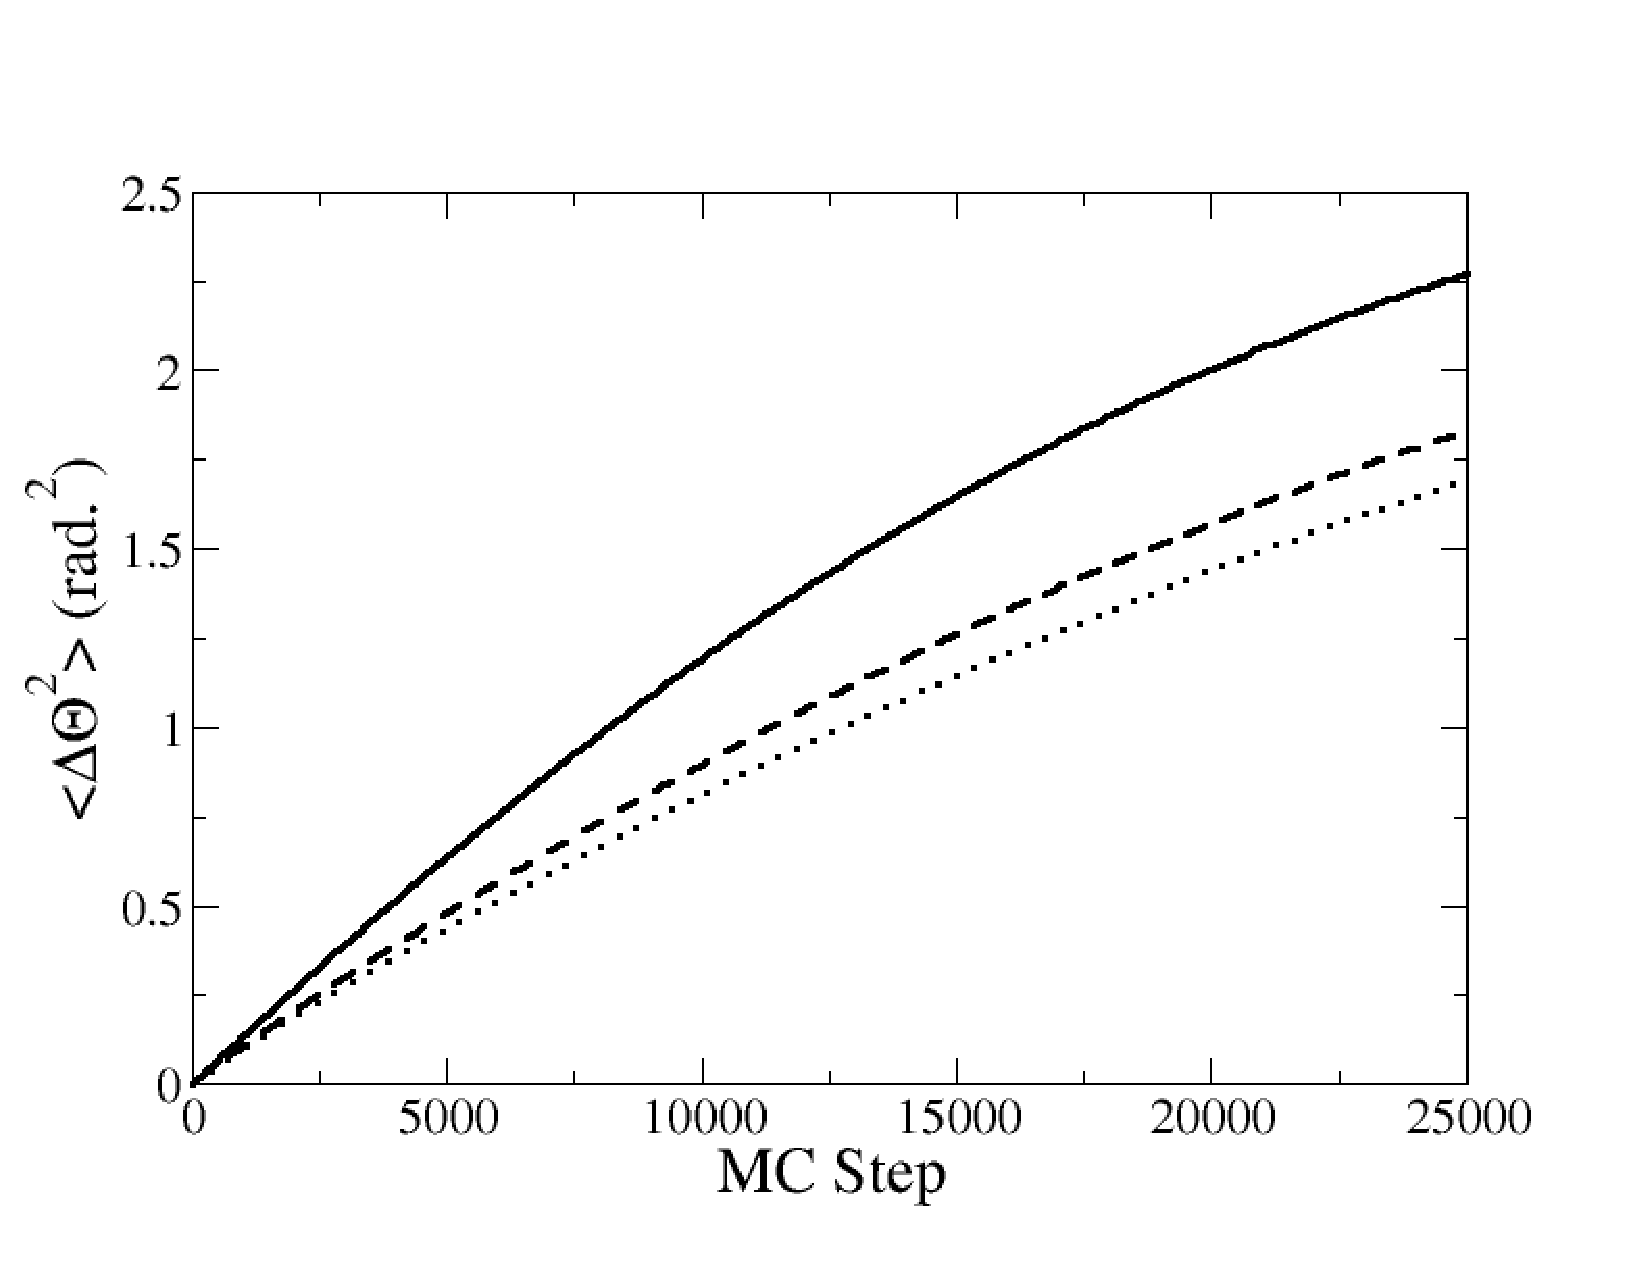
\includegraphics[width=0.6\textwidth]{disorder/rot.pdf}
		\label{rot}
	}

	\subfloat[]{
		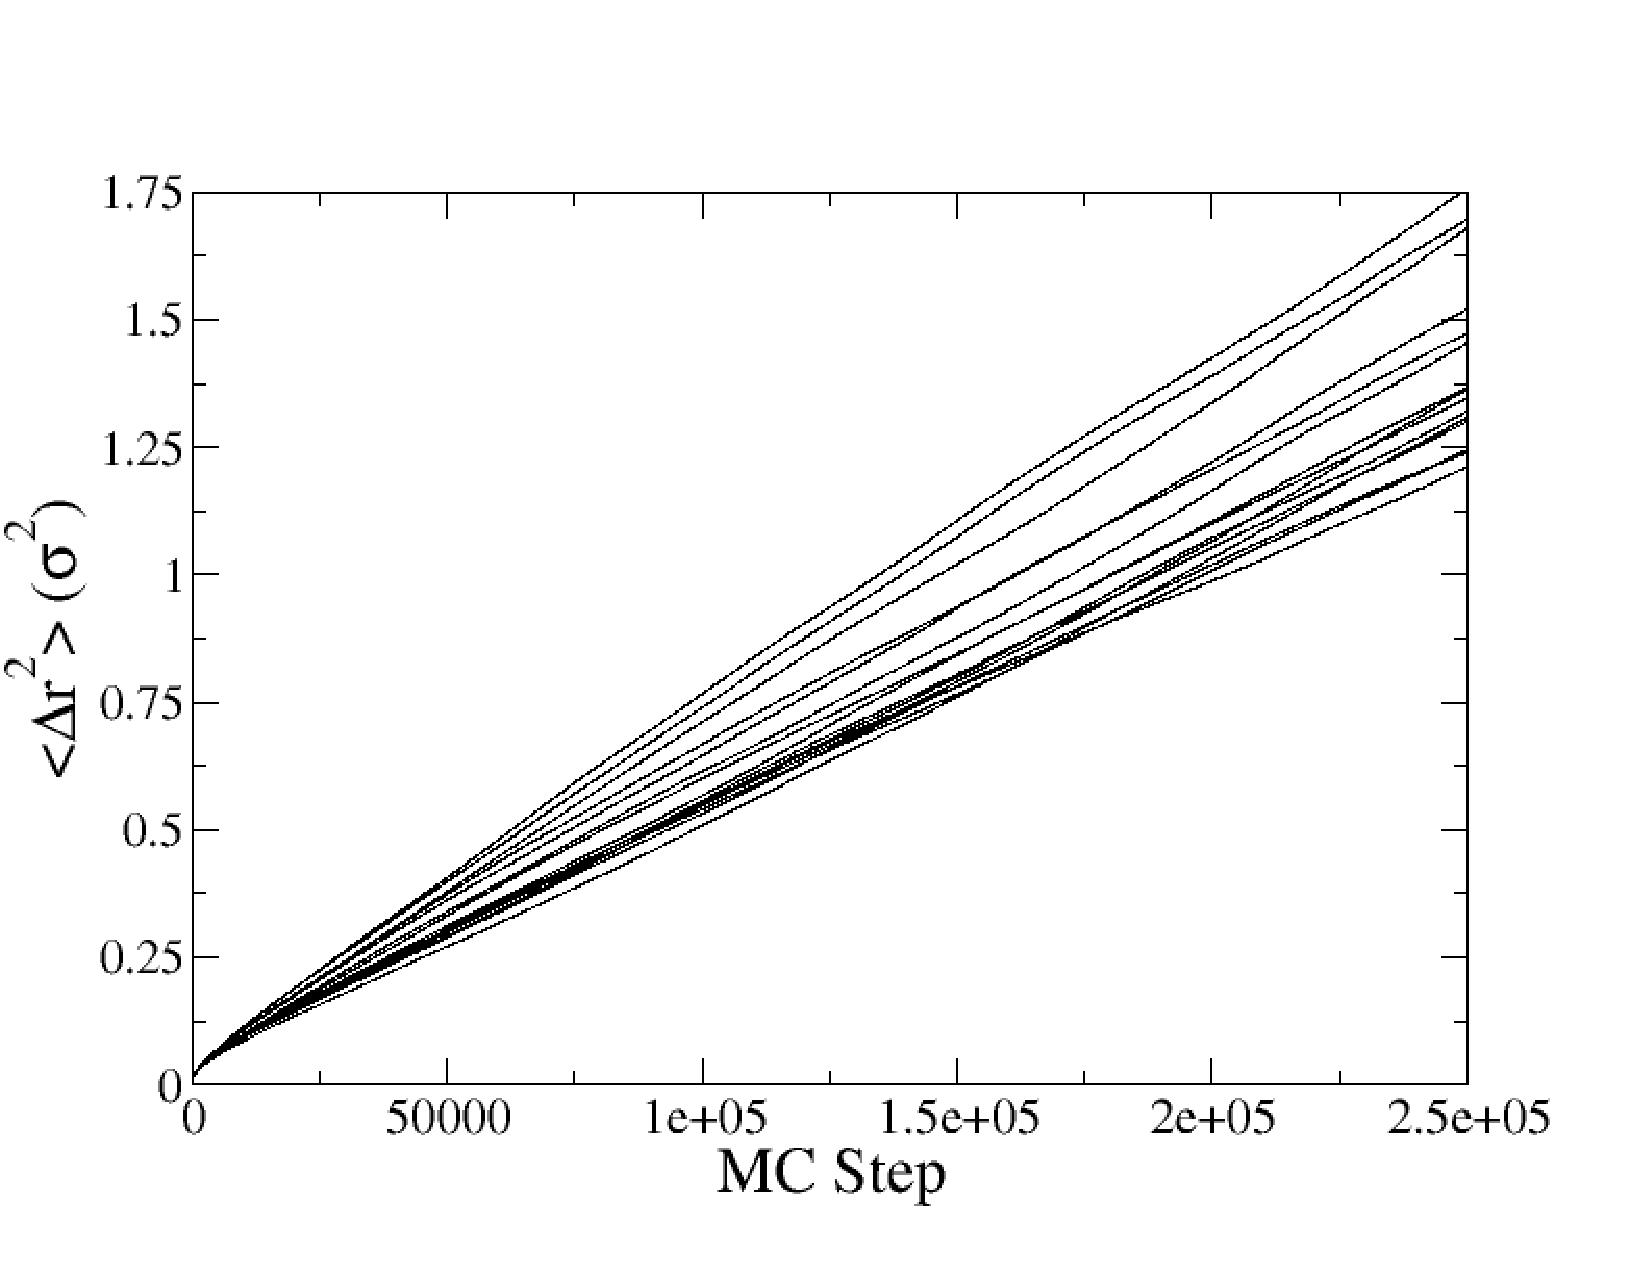
\includegraphics[width=0.6\textwidth]{disorder/trans.pdf}
		\label{trans}
	}\end{center}
	\caption[Rotational and translational diffusion for aspherical particles]{\subref{rot} Rotational mean square displacement for a subset of the particles considered. The solid line is a 
	reference for nearly spherical particles. The dashed line is the result for  those particles that  
	 crystallized and the dotted line shows $\left<\Delta\theta^2\right>$ for those that did not.
  The data were averaged over 20 realizations in each region under the same pressure $P^*=20$.
\subref{trans} Translational mean square displacement for  20 different particle shapes that failed to crystallize.}\label{diff}
\end{figure}

To address the first question, we measured the rotational diffusion, $\left<\Delta\theta^2\right>$, for 20 systems 
that crystallize, all at a reduced pressure $P^* = 20$ and near the phase boundary.  As a reference 
we also plotted  $\left<\Delta\theta^2\right>$ for nearly spherical particles, obtained by setting $\sigma_0 = 10^{-4}\sigma$, 
where we know particles are free to rotate at their lattice sites.

As can be seen in Figure~\ref{rot}, we find no evidence that particles in the crystalline phase become 
orientationally arrested or manifest an orientationally anomalous behavior. The only effect is that of decreasing their diffusion constant, 
but this is expected from simple geometrical considerations. It is obvious that at very large densities, 
regardless of the specific phase a system selects, particles' orientations will manifest a glassy behavior or eventually freeze.~\cite{schweitzer} 

It is therefore of interest to also look at the dynamical
properties of those particles in systems which do not crystallize and are located 
just across the phase boundary from the ones that do crystallize. 
These results, obtained at the same reduced pressure $P^*=20$, are also shown in Figure~\ref{rot}. 
We find no signature of anomalous dynamics, neither in the rotational (Figure~\ref{rot}), nor in the translational 
(Figure~\ref{trans}) degrees of freedom; that is, such systems behave as regular fluids.

This rotational plasticity in crystals of these aspherical particles provides and explanation for why the results of the polydisperse systems studied in Section~\ref{sec:polydisperse} applied to the monodisperse systems studied in Sections~\ref{sec:disorderpress} and~\ref{sec:disorderyesno}.
The practical effect of this fact is  
that any two identical neighboring particles will typically be misoriented and face each other with random regions of their respective surfaces. 
As a consequence, their mutual interaction becomes  hardly distinguishable, on average, from that of two particles with different shape, thus explaining why monodisperse and polydisperse 
systems may indeed present analogous equilibrium properties. 

Note, however, the deviations from the predicted pattern in Figure~\ref{mono2}
 at  the extreme ends of $Aq$,  corresponding to particle shapes that have values of $q$ significantly 
different from the average $q$ of the distribution. The deviation at large $q$ is expected as the analogous behavior is observed for polydisperse systems;
as particles become more anisotropic their rotational degrees of freedom are reduced until they perfectly align in the $q\rightarrow 1$ (rod) limit, making 
the averaged random-shape argument described above inappropriate.

A  bit more surprising is the deviation for very small values of $q$, for which we find that the polydisperse system with $N_b=12$ nicely follows the master curve.
To rationalize this behavior one has to realize that for small values of $N_b$, when $q\rightarrow 0$, particles tend to acquire rather symmetric and specific geometries, such as platonic solids, which 
also require orientational ordering  to tile the space as soon as $A$ becomes sufficiently large. These specific particle shapes dominate the shape space for $q\sim 0$ and small values of $N_b$,
and lead to deviations from the inverse power law behavior.  

This result is by no means conclusive, as a thorough investigation of this last point would require larger system sizes 
and an event-driven dynamics of the components.  Our results seem to suggest that what sets the location of 
the phase boundary is not a sudden slowdown of the dynamics of the system, but more likely
 an increase of the Gibbs free energy difference between the crystalline  and the fluid phase, analogous to
that found for polydisperse spherical particles~\cite{frenkel2}. 
It would be interesting to investigate the equilibrium properties and the stability of 
candidate crystalline structures for different values of $A$ and $q$ to investigate whether our boundary line 
coincides with the onset of crystal instability, but for the reasons given above, we have not attempted to do so.


\section{Conclusions}

To conclude, out data represent a first step in attempting to understand how deviations from asphericity affect the thermodynamics of crystallization of particle systems.
Our results show  that the coexistence pressure of systems of monodisperse and shape-polydisperse particles is remarkably well-described, within the limits described above,   
 by a simple first order Taylor expansion in terms of $Aq$, $\frac{p^* - p^*_{HS}}{p^*_{HS}} = \alpha Aq + ...$

Apart from the details concerning the dynamics of these systems, our results show that, for aspherical particles,
shape and crystallizability can be directly and easily correlated when particles are characterized in terms of their
asphericity via $q$ and $A$. Our data suggest precise limits for the manufacture of nanocomponents expected to crystallize, which should be experimentally testable,
and may have important implications for the problem of protein crystallization. 
The latter system is clearly far more complex  than the one explored here,
since not only shape, but also interparticle direct interactions (which are not necessarily isotropic), 
are responsible for the organization of proteins into large macroscopic crystals. Nevertheless, it would be
interesting to systematically explore to what extent  a similar correlation exists in this case.   

Finally, a further avenue of study, and one that is vital to truly understanding phenomena surrounding crystallization of these particles, has to do with the free volume available in a crystal.
As discussed in Section~\ref{sec:CNT}, the chemical potential difference between the fluid and crystalline phases, which is a vital consideration in the crystallization, is determined, in purely repulsive systems such as these, by the free volume available per particle in the crystal versus that available to the ``jammed'' fluid at the same density.

This is not a trivial quantity to compute in complicated systems such as these, and will be very sensitive to details about how, precisely, it is calculated.
For example, it might be necessary to attempt to calculate an ``accessible'' volume of each particle, in analogy to solvent-accessible volumes in proteins, which accounts for the fact that a narrow, deep cleft, for example, should have no bearing on the way in which two particles of the same size interact with each other.
However, this would be a vital step toward a complete theoretical understanding of the problem, and work in this direction is currently underway.


%\chapter{Two-Dimensional Packing of Soft Particles and the Soft Generalized Thomson Problem}
\chapter{Two-dimensional packing of soft particles on planes and spheres}
\label{chap:2dsoft}

\section{Introduction}
Understanding how nanocomponents spontaneously organize into complex macroscopic structures
is one of the great challenges in the field of soft matter today. Indeed, the ability to predict and control 
the phase behavior of a solution, given a set of components, may open the way to the development
of materials with novel optical, mechanical, and electronic properties. 

Of particular interest for optical applications are the crystalline phases. Until recently, it was believed that 
shape anisotropy and/or directional interactions were key elements for the formation of 
crystals with complex symmetries commonly observed, for instance, in atomic solids. 

The study of
the phase behavior of components interacting with exotic (yet isotropic) potentials has 
proven this belief to be incorrect. For instance,
Torquato \textit{et al.} have shown, using inverse optimization techniques, that it is possible to achieve
non-close-packed structures such as simple cubic, hexagonal,  wurtzite and even diamond phases
with isotropic pair potentials  (see ref~\cite{torquato} for a review on the subject). 
Furthermore, spherical particles interacting via a hard core and a repulsive shoulder potential are known to organize into complex mesophases not unlike those found with diblock copolymers~\cite{glaser2}. 

One class of pair potentials that has recently attracted much attention  
is that describing the interactions between soft/deformable mesoparticles. 
Unlike  typical colloidal particles for which excluded volume interactions are strictly enforced via a hard-core or a Lennard-Jones potential,  complex mesoparticles such as charged or neutral star polymers, dendrimers or microgels present a more peculiar pair potential describing their volume interactions. 
Surprisingly, the simple relaxation of the constraint of mutual impenetrability between isotropic 
components gives access to several non-close-packed crystalline structures at high densities.

Given the complexity of these mesoparticles, their interactions are usually 
extracted via an explicit coarse-grained procedure to obtain ad hoc effective pair potentials. 
What emerges is a great variety of nontrivial interactions, some of which allow for even 
complete overlap among the components, resulting in a very rich phenomenological behavior.
Remarkably, it is feasible to engineer interactions between star polymers or dendrimers
by controlling their overall chemical and topological properties~\cite{mladek}. 
   
The phase behavior of several systems adopting these exotic, but physically inspired, interactions
has been the subject of several publications~\cite{louis,likos0,richter,likosB,denton,gottawald,pierleoni, bozorgui, capone, xu,prestipino}. 
Notably, it was found that some classes  of soft interactions lead 
to  reentrant melting transitions, others to polymorphic cluster phases~\cite{mladek2}, and in general to multiple  transitions 
involving close-packed and non-close-packed crystalline phases~\cite{suto,LikosNat,pephertz} as a function of the system density.  

Remarkably,  the phase behavior of these systems is very much dependent on the shape of the pair potential. 
\citeauthor{likos}~\cite{likos} established a criterion 
to predict whether for a bounded and repulsive potential reentrant melting or cluster phases will occur based
on the sign of the Fourier transform of the interaction.
Nevertheless, there is currently no method to predict \textit{a priori} what specific crystal structures may become 
accessible for a given potential. 
For a recent review on the subject we refer the reader to reference~\cite{LikosRev}. 
  
{The main idea behind the formulation of the criterion is that at large densities each particle is typically  interacting with such a 
significant  number of neighbors that the simple mean field approximation (MFA) for the excess free energy of the system becomes quite accurate.
Under this approximation, the internal energy of the system
\begin{equation}
	F_{\textrm {ex}}\left[\rho({\bf {r}})\right] \simeq \frac{1}{2}\int d{\bf {r}} d{\bf {r'}} V(\left|{\bf {r}} - {\bf {r'}}\right|)\rho({\bf {r}}) \rho({\bf {r'}}) \,,
\end{equation}
where $\rho(\bf{r})$ is the density profile of the system and is assumed not to vary too rapidly with respect to the particle size $\sigma$, and the approximation for $F_{\textrm {ex}}$ gets more accurate for higher densities $\rho$.
This leads to a pair correlation function with a very simple form
\begin{equation}
	c(\left|{\bf{r}}-{\bf{r'}}\right|;\rho) \equiv \lim_{\rho({\bf{r}}) \rightarrow \rho} \frac{\partial^2 \beta F_{\textrm{ex}}\left[\rho\left({\bf{r}}\right)\right]}{\partial \rho({\bf{r}}) \partial \rho({\bf{r'}})} = -\beta V(r) \,. 
\end{equation}
The Ornstein-Zernike relation, which relates the Fourier transform of the total correlation function, $\tilde{h}(q)$, to the Fourier transform of the pair correlation function, $\tilde{c}(q)$, takes the form
\begin{equation}
	\tilde{h}(q) = \frac{\tilde{c}(q)}{1 - \rho \tilde{c}(q)} \,.
\end{equation}

The static structure factor $S(q)$ can then be related to $\tilde{h}(q)$, resulting in a simple functional form
\begin{align}
	S(q) &\equiv 1 + \rho\tilde{h}(q) = 1 + \frac{-\rho \beta \tilde{V}(q)}{1 - \rho \beta\tilde{V}(q)} \notag \\
	&= \frac{1}{1 + \beta\rho\tilde{V}(q)} \,. \label{Sdef}
\end{align}
This simple expression for $S(q)$ allows one to deduce several  properties of the fluid phase.

For instance, the instability of the fluid phase (and thus crystallization of the fluid) is indicating by a singularity in $S(q)$.
However, when the MFA holds, Equation~\ref{Sdef} indicates that a singularity in $S(q)$ will occur when $\beta\rho\tilde{V}(q) = -1$.

This means that, if $\tilde{V}(q)$ is positive defined for all $q$, then for any temperature or density at which the MFA becomes exact, the fluid phase will be the most stable phase.
Solid phases are possible when the MFA becomes inaccurate or for potentials which have non-positive-defined Fourier transform.
Thus, if a potential with a positive-defined Fourier transform passes from a state in which the MFA is inaccurate to one in which it holds, it is possible to have reentrant melting, in which, as a function of increasing density (for example), the system passes from the fluid phase, through a crystalline phases, and then back to the fluid phase.
For more details on the subject we refer the reader to~\cite{likos}.} 

In this chapter we focus on two-dimensional systems.
Although much of the research in this field has focused on three-dimensional systems,
earlier numerical work on particles interacting via a hard core plus a shoulder potential
in two dimensions has revealed 
a phenomenological behavior that can be as rich as that observed at higher dimensionality
~\cite{Malescio,Stell,jagla,glaser}. 

Here we focus on  bounded soft potentials. Specifically, expanding on recent results 
on Hertzian spheres~\cite{pephertz} and dumbbells~\cite{saric2} in three dimensions, we analyze the phase behavior of soft
elastic particles in two dimensions. We generalize our results to spherical surfaces,  and 
discuss the generalized Thomson problem for our soft potentials  by identifying novel polyhedral structures
representing minimal energy configurations formed by soft particles constrained on the surface of a sphere at different packing densities.
{Although the term ``packing'' generally refers to hard-particle or weakly compressed systems, here it should be understood to be describing the ordering of highly compressed soft and deformable particles.}

\section{Simulation details}
To study the phase behavior of soft nanoparticles in two dimensions we performed numerical simulations.
We considered systems of at least $N=1000$ spherical particles and used the 
standard Monte Carlo method {with random initial configuration} in the NPT and NVT ensemble for the planar and spherical case, respectively.
{Results for two-dimensional systems were reproduced starting from a square-crystal initial configuration.}
All simulations where run for a minimum of $10^6$ iterations.

Any two particles in our system interact
via a generalized version of Hertz potential. The Hertz potential describes the elastic energy penalty associated with an axial compression
of two deformable spheres. Its functional form can be generalized as follows
 \begin{equation} \label{Hertz}
	V(r)= 
		\begin{cases}
  			\varepsilon(1-\frac{r}{\sigma})^{\alpha} & \text{for } r \leq \sigma\cr
			0 & \text{for } r  > \sigma\cr
		\end{cases} \,,
\end{equation}
where $\sigma$ is the particle diameter, $r$ is the interparticle distance, $\varepsilon$ is the unit of energy, 
and $\alpha$ is a 
parameter that we control to modulate the shape of the interaction. The elastic (Hertzian)
case is recovered for $\alpha=\frac{5}{2}$. 

The Hertz model,  developed to account for small elastic deformations,
becomes inaccurate when associated to the large overlaps among particles that is
achieved at large densities, which will be discussed further in Section~\ref{sec:hertzprobs}; nevertheless, it provides us with a simple representation of a 
finite-ranged, bounded soft potential with a positive definite Fourier transform 
(a condition that guarantees reentrant melting in the phase diagram~\cite{likos}). 
We included in our study two more values of $\alpha$ to account for a slightly harder 
($\alpha=\frac{3}{2}$) and a slightly weaker ($\alpha=\frac{7}{2}$) potential than the elastic one ($\alpha=\frac{5}{2}$).
Figure~\ref{pot} shows these potentials. 
  
Crystallization in our simulations was determined using a combination of visual inspection and numerical order parameters similar to those described in~\cite{binder}, which can be seen as a simpler, two-dimensional version of those described in Section~\ref{sec:orderparamdesc}. Specifically,  given a randomly chosen particle $j$, and a reference direction set to be along the bond between this particle and one of its nearest neighbors, we can define an order parameter sensitive to a crystal of $D$-fold symmetry (specifically six-fold hexagonal and four-fold square crystals) as follows.

For all particles $k$ within a radius of some cutoff $r_c$ of $j$ (including $j$ itself), we calculate the angle 
$\phi_{lk}$ between the bond joining each of the $D$ nearest neighbors $l$ of $k$ to $k$ and the reference direction.
If the number of particles within $r_c$ of $j$ is $N_k$, then the order parameter $\Psi_D^j$ is given by:
{\begin{equation}
	\Psi_D^j = \frac{1}{N_k}\frac{1}{D} \left|\sum_{k} \sum_{l} e^{i D \phi_{lk}}\right| \,.
\end{equation}
This process is then repeated $N$ times and an average $\Psi_D$ is calculated, yielding a value between $0$ (for completely disordered systems) and $1$ (for perfectly crystalline systems).

This order parameter is analogous to that defined in~\cite{binder} except that instead of $\Psi_D^i$ being an average over all particles $k$ in the system, it is only over particles $k$ within $r_c$ ($= 1.65\sigma$ in our case); thus it is ``semi-local'' and allows crystalline order to be detected even in the presence of metastable grain boundaries.
The order parameter in~\cite{binder} represents the $r_c \rightarrow \infty$ limit of the above method.
\begin{figure}
	\begin{center}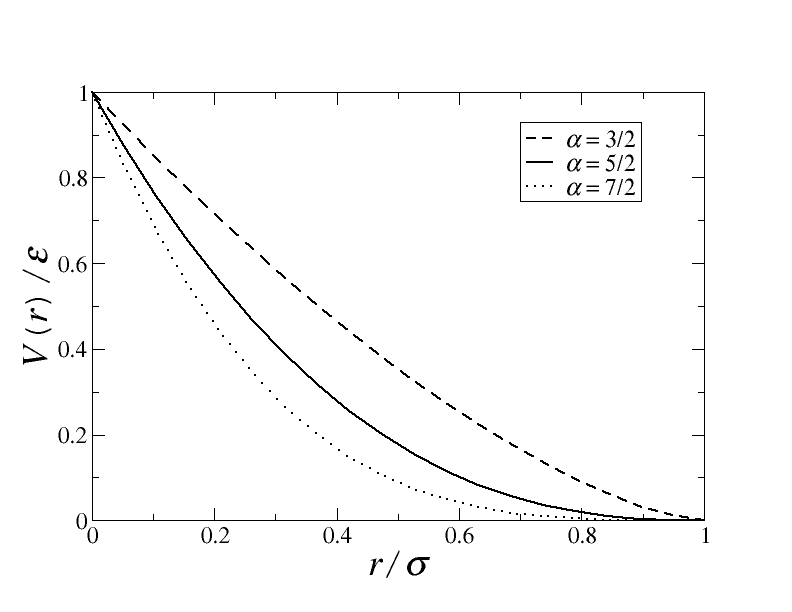
\includegraphics[width=0.6\textwidth]{2dsoft/potential.png}\end{center}
	\caption[Rescaled potential $\frac{V(r)}{\varepsilon}$ for the three values of $\alpha$ used in this study]{Plot of the rescaled  pair potential $\frac{V(r)}{\varepsilon}=(1-\frac{r}{\sigma})^{\alpha}$ 
	for the three values of $\alpha$ used in this study: $\alpha =\left\{\frac{3}{2}, \frac{5}{2}, \frac{7}{2}\right\}$}\label{pot}
\end{figure}
 
To draw the phase diagrams we scan the phase space defined by the rescaled temperature 
$T_{\rm r}=\frac{k_{\rm B}T}{\varepsilon}$ and the rescaled number density $\rho_{\rm r}=\frac{N\sigma^2}{A}$ (where $A$ is the area of the system) to evaluate the several phases of the system in terms (when possible) of its order parameter 
$\Psi_D$.
{The phase of the system was evaluated on a grid with a resolution of 0.001 in $T_{\rm r}$ and roughly 0.25 in $\rho_{\rm r}$.}
The lines separating the different regions are guides to the eye{, and are placed between data points relative to structures having different symmetry}. 

Given the peculiarities of phase transitions in two dimensions, and the richness in the phases behavior reported, we have not attempted to establish equilibrium boundaries between the different phases, yet we
have reproduced our results using molecular dynamics simulations with a Langevin thermostat performed in key regions of the phase space, and compared the stability of the crystalline structures by measuring their relative energies at $T_{\rm r}\rightarrow 0$.

{Because thermodynamic phase diagrams are not presented, the phase diagrams that follow should be considered as semi-qualitative illustrations of the variety of phases which occur and the trend with which their occurrence follows the system density; specifics of the slopes and the precise location of the dividing lines between phases would require a more accurate study of the thermodynamic stability of the phases.}

{For the simulations of the generalized Thomson problem in the latter half of the chapter (Section~\ref{sec:thomson}), a temperature quench was performed from a relatively high temperature ($T_r = 0.1$) to a very low temperature ($T_r = 10^{-7}$) in order to approach the zero-temperature limit.
For each $r_0$, the system was simulated with three initial configurations; one random, and one each from the structure obtained at slightly larger and slightly smaller $r_0$.}

\section{Soft particles in planar geometries}

\begin{figure}
 	\begin{center}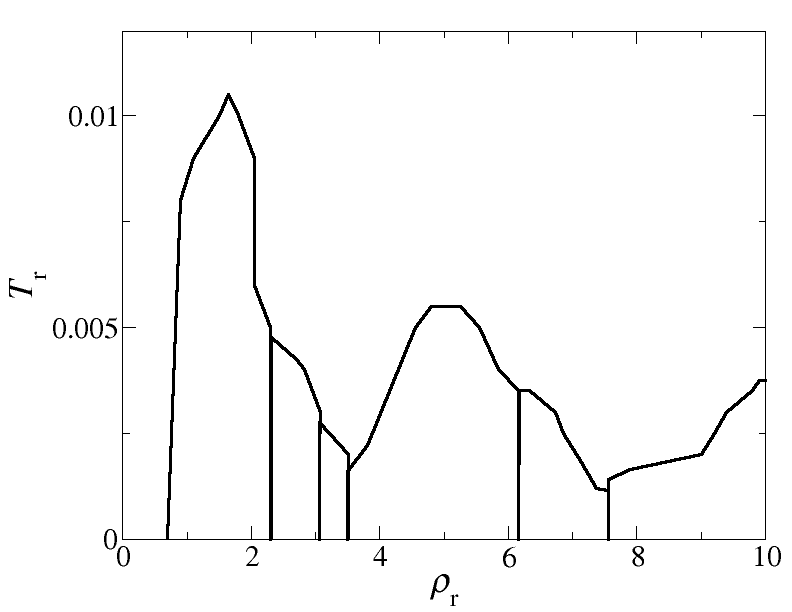
\includegraphics[width=0.6\textwidth]{2dsoft/fivehalvesdens.png}
		\label{fivehalvesdens}
		\put(-195,35){\subref*{triangular}}
		\put(-170,35){\subref*{square}}
		\put(-157,35){\subref*{pent}}
		\put(-125,35){\subref*{triangular}}
		\put(-81,35){\subref*{square}}
		\put(-33,35){\subref*{triangular}}\end{center}
	\caption[Temperature vs. number density for $\alpha = \frac{5}{2}$]{Temperature vs. number density phase diagrams for two-dimensional particles interacting via a Hertz potential ($\alpha=\frac{5}{2}$). Labels on the plots refer to the labels of the phases in Figure~\ref{phasep}.}\label{phaseHertz}  
\end{figure}

We begin by presenting the phase diagram for the case of Hertzian (elastic) spheres.
The result is shown in Figure~\ref{phaseHertz}.
The labels in the figure refer to the structures shown in Figure~\ref{phasep}. 
As expected from Likos' criterion~\cite{likos} our system shows reentrant melting behavior
and a maximum temperature above which the system remains fluid at all densities.
   
   
The phase behavior reported here is qualitatively similar to that observed in three dimensions;
however, the two-dimensional system does not produce a phase space that is as structurally rich  as its three dimensional counterpart. 
Across the spectrum of  densities (up to $\rho_{\rm r}=10$) and temperatures (down to 
$T_{\rm r}=10^{-6}$) that we explored, we find multiple crystal-to-crystal 
transitions from hexagonal (phase~\subref{triangular}) to square symmetry (phase~\subref{square}). 
Interestingly,  the occurrence of the two phases has an alternating periodic pattern, and no isostructural transition was detected in our system~\cite{mladek3}.
{The multiple occurrences of a single phase (for example, phases~\subref{triangular} and~\subref{square} in Figure~\ref{phaseHertz}) are identical except for uniform scaling of the interparticle distances as the density of the system is changed.}

This pattern is only broken at a small range of densities centered around $\rho_{\rm r}\simeq 3.25$.
This region (phase~\subref{pent}) is characterized by a complex structure dominated by particles arranged mostly into
pentagonal units. The color coding of the phase shown in Figure~\ref{pent} helps in rationalizing the overall
symmetry of the structure which in this representation can be thought of as the combination of four 
square lattices. Three lattices are generated by pentagonal units, displaced with
respect to each other but  oriented along the same axis. The fourth lattice is built out
 of the non-connected particles and is oriented along an axis 
 that forms an angle of 45 degrees with the other lattices. 

\begin{figure}
	\begin{center}\subfloat[]{
		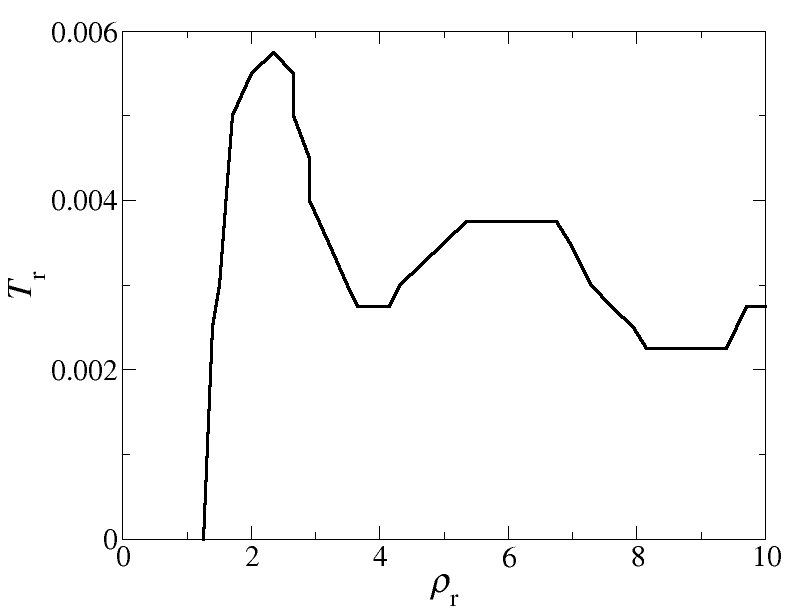
\includegraphics[width=0.6\textwidth]{2dsoft/sevenhalvesdens.png}
		\label{sevenhalvesdens}
		\put(-120,60){\subref*{triangular}}
	}

	\subfloat[]{	
	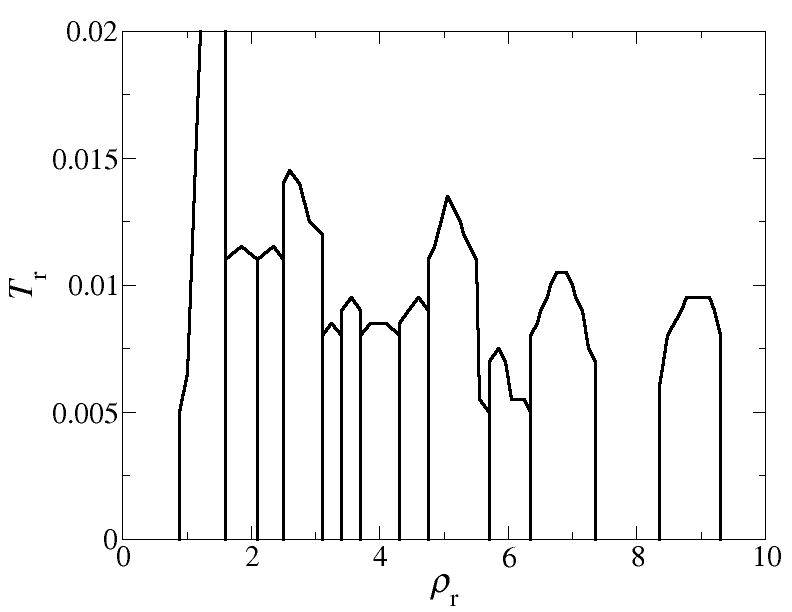
\includegraphics[width=0.6\textwidth]{2dsoft/threehalvesdens.png}
	\label{threehalvesdens}
	\put(-200,40){\subref*{triangular}}
	\put(-188,40){\subref*{square}}
	\put(-178,40){\subref*{line}}
	\put(-168,40){\subref*{honey}}
	\put(-158,40){\subref*{kagome}}
	\put(-151,40){\subref*{largesquare}} 
	\put(-142,40){\subref*{snub}}
	\put(-131,40){\subref*{triangular}}
	\put(-118,40){\subref*{square}}
	\put(-100,40){\subref*{pent}}
	\put(-84,40){\subref*{honey}}
	\put(-40,40){\subref*{triangular}}	
	}\end{center}
	\caption[Temperature vs. number density for $\alpha = \frac{3}{2}$ and $\alpha = \frac{7}{2}$]{Temperature vs. number density phase diagrams for two-dimensional particles interacting via   the generalized Hertz potential  with \subref{sevenhalvesdens} $\alpha =\frac{7}{2}$ and  \subref{threehalvesdens} $\alpha=\frac{3}{2}$.  
Labels on the plots refer to the labels of the phases in Figure~\ref{phasep}.}\label{phased} 	
\end{figure}

To understand how the phase behavior is affected by the specific choice of the functional 
form of the potential, we repeated the calculation of the phase diagram for 
$\alpha=\frac{7}{2}$ and $\alpha=\frac{3}{2}$.
The results are presented is Figure~\ref{phased}.

Although the overall
trend is very similar, the number and the sequence of phases that we find are significantly different.
Namely, $\alpha=\frac{3}{2}$ leads to a significantly richer structural behavior, while the 
larger value of $\alpha$ results in a single hexagonal crystalline structure; however, even for the $\alpha = \frac{7}{2}$ case, we observe a complicated variety of reentrant behaviors.

As a reference, notice  that our potential tends  to the linear-ramp potential for $\alpha=1$
(for which a large number of phases including quasi-crystals have been observed~\cite{jagla}), we recover the square-shoulder potential for $\alpha\rightarrow 0$
(for which a cascade of cluster phases are expected), and tends to a Kronecker delta potential
for  $\alpha\rightarrow\infty$ (for which no crystallization is expected at any finite density).

\begin{figure*}
	\begin{center}
	\subfloat[Hexagonal]{
		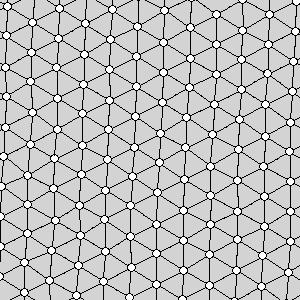
\includegraphics[width=0.3\textwidth]{2dsoft/triangular.png}
		\label{triangular}
	}
	\subfloat[Square]{
		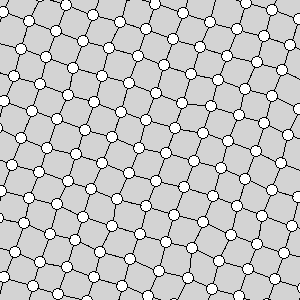
\includegraphics[width=0.3\textwidth]{2dsoft/square.png}
		\label{square}

	} 
	\subfloat[Lines]{
		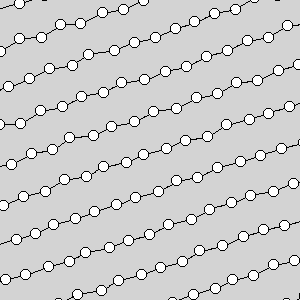
\includegraphics[width=0.3\textwidth]{2dsoft/line.png}
		\label{line}
	}

	\subfloat[Stretched honeycomb]{
		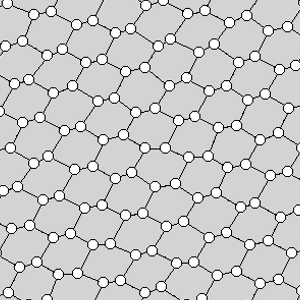
\includegraphics[width=0.3\textwidth]{2dsoft/honey.png}
		\label{honey}
	}
	\subfloat[Kagome]{
		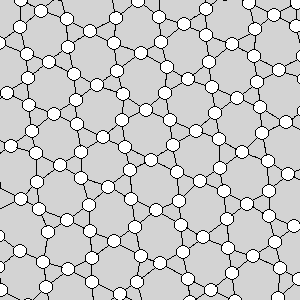
\includegraphics[width=0.3\textwidth]{2dsoft/kagome.png}
		\label{kagome}
	}
	\subfloat[Open square]{
		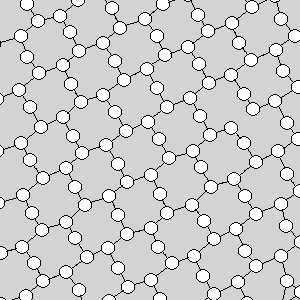
\includegraphics[width=0.3\textwidth]{2dsoft/largesquare.png}
		\label{largesquare}
	}

	\subfloat[Snub square]{
		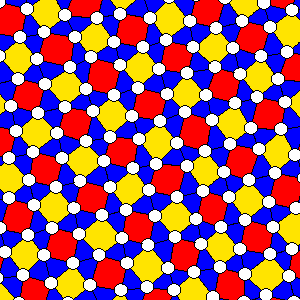
\includegraphics[width=0.3\textwidth]{2dsoft/snub.png}
		\label{snub}
	}
	\subfloat[Pentagons]{
		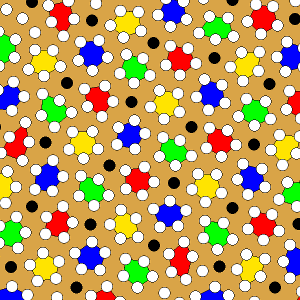
\includegraphics[width=0.3\textwidth]{2dsoft/pent2.png}
		\label{pent}
	}
	\end{center}
	\caption[Two-dimensional crystal phases formed in these systems]{Two-dimensional crystal phases formed in these systems.}\label{phasep}
\end{figure*}

At least as a general trend, it is therefore not surprising that structural 
variety increases for smaller values of $\alpha$. In this regard, it is interesting to estimate
the critical power above which the hexagonal lattice becomes the only stable lattice as observed 
in Figure~\ref{sevenhalvesdens}.

Given that the only other competing structure at large values of $\alpha$ is the square lattice, we
computed the energy density difference between hexagonal and square lattices as a function of
density and at zero temperature for different values of $\alpha$. The result is presented
 in Figure~\ref{energies} for densities up to $\rho_{\rm r}=25$ (our full numerical data extend up
 to $\rho_{\rm r}=100$, but are not shown for the sake of clarity).
We find that the hexagonal lattice becomes more stable than the square lattice at all 
densities for any powers above the onset value $\alpha^*\simeq 3.182$. 

Several numerical simulations at finite densities for powers ranging from $\alpha=10$ to $\alpha=50$ 
where carried out, and indeed only hexagonal structures where observed upon system ordering.
The presence of reentrant melting was also established for $\alpha=5$ and $\alpha=10$.
The oscillating behavior  of the energy density difference for $\alpha<\alpha^*$ also explains 
qualitatively the periodic structural pattern observed in the phase diagram for $\alpha=\frac{5}{2}$. 

{The precise underlying physical origin of this periodic structural pattern is currently under further investigation.
Early results indicate that the finite range of the potential is a significant contributor to the behavior; in particular, the fact that as the density of the system increases, the number of particles with which each particle in the system can interact increases in a stepwise fashion.}


\begin{figure}
\begin{center}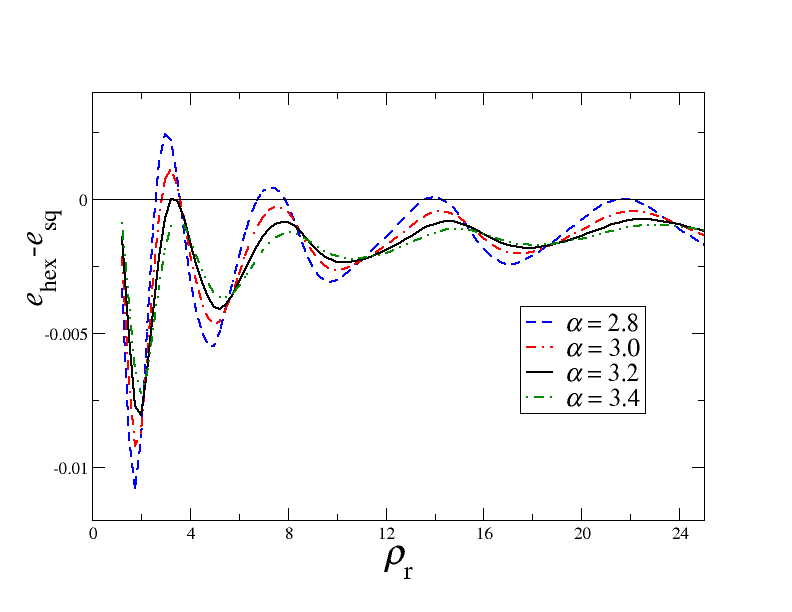
\includegraphics[width=0.8\textwidth]{2dsoft/energies.png}\end{center}
\caption[Energy density difference between hexagonal and square lattices vs. $\alpha$]{Energy density difference between hexagonal and square lattice at $T_{\rm r}=0$ as a 
function of system density at different values of $\alpha$. The 
critical $\alpha$ is estimated to be around $\alpha\simeq 3.1822$.}
\label{energies}
\end{figure}

\section{Soft particles on spheres: the soft generalized Thomson problem}\label{sec:thomson}

We now turn to the discussion of the second part of this chapter. Given the structural variety
observed in the two-dimensional compression of soft nanoparticles, it is interesting to 
extend our results to other geometries. The spherical case is of particular interest 
because a large body of work has been dedicated to finding and enumerating minimal 
energy conformations of particles constrained over a spherical shell, and 
repelling each other via an electrostatic repulsion ~\cite{altschuler, erber, perez-garrido, morris, erber2, edmundson, altschuler2, dodgson, perez-garrido2, perez-garrido3,Bowick2,Bowick3}.

This is what Thomson asked in 1904~\cite{thomson} when attempting to construct his plum pudding
model of the atom. Although there is consensus on the minimal energy structures for
$N<100$, the problem becomes more involved for large values of $N$ for which an exponentially large
number of low energy configurations becomes available.  In this regime, lattices with overall icosahedral
symmetry ({\it icosadeltahedra}) have been initially postulated as possible global minima for
specific magic number of particles~\cite{altschuler2},  but eventually 
it was shown that it is possible to lower the energy of these configurations by adding dislocation 
defects~\cite{perez-garrido3,Bowick}. Grain boundary scars have also been observed in
experiments~\cite{bausch}.
It is important to note that the lowest-energy structure depends only on the number of particles, not the size of the sphere on which they are fixed.
 
\begin{figure*}
	\begin{center}
	\subfloat[]{
	\includegraphics[width=0.45\textwidth]{2dsoft/Ssquare.png}\label{Ssquare}
	} 
	\subfloat[]{	
	\includegraphics[width=0.45\textwidth]{2dsoft/Schain.png}\label{Schain}
	}

	\subfloat[]{	
	\includegraphics[width=0.45\textwidth]{2dsoft/Skagome.png}\label{Skagome}
	}
	\end{center}
\caption[Snapshots of soft particles on a spherical surface]{Snapshots of soft particles packing on a spherical surface.
Here we show ~\subref{Ssquare}~square, \subref{Schain}~open square and \subref{Skagome}~kagome lattices.}\label{spheres}	
\end{figure*}

Although we confirm that the same pattern of phases obtained in two dimensions 
also develops on large areas of spherical shells -- apart from the topologically required defects --
as a function of  the radius of the sphere (see Figure~\ref{spheres} for a sample of these configurations), we have not attempted to 
enumerate all possible low energy states for large $N$. It is, however, clear that considering
soft potentials introduces two new parameters to the system: namely the packing density and the 
shape of the potential. A careful analysis of the defects and symmetries arising in this 
regime is the subject of future investigation; here we focus on
the case of small number of particles $N\leq12$ for $\alpha=\frac{3}{2}$ and $\alpha=\frac{5}{2}$.

\begin{figure*}
\tiny\begin{tabular}{>{\centering}m{12px} | >{\centering}m{0.12\textwidth} >{\centering}m{0.12\textwidth} >{\centering}m{0.12\textwidth} >{\centering}m{0.12\textwidth} >{\centering}m{0.12\textwidth} >{\centering}m{0.12\textwidth} >{\centering}m{0px} }
$N_b$ & \multicolumn{6}{c}{Cluster geometry} \\
\hline
\multirow{4}{*}{5} & \includegraphics[width=0.10\textwidth]{2dsoft/5a.png} & \includegraphics[width=0.10\textwidth]{2dsoft/5b.png} &  \inbox{\includegraphics[width=0.10\textwidth]{2dsoft/5c.png}} & & &\\
%& square pyramid & $P_{\rm A}^{(5)}$ & \inbox{trigonal dipyramid} & & & &\\
& $r_0 = 0.65$ & $r_0 = 0.58$ & \inbox{$r_0 = 0.50$} & & & &\\
& $E = 0.116675$ & $E = 0.457195$ & \inbox{$E = 1.098194$} & & & &\\
\cline{4-4}\\[-7pt]

\cline{3-3}
& & \inbox{} & & & & &\\[-7pt]
\multirow{4}{*}{7} & \includegraphics[width=0.10\textwidth]{2dsoft/7a.png} & \inbox{\includegraphics[width=0.10\textwidth]{2dsoft/7b.png}} & \includegraphics[width=0.10\textwidth]{2dsoft/7c.png} & \includegraphics[width=0.10\textwidth]{2dsoft/7d.png} & \includegraphics[width=0.10\textwidth]{2dsoft/7c.png} & \includegraphics[width=0.10\textwidth]{2dsoft/7a.png}& \\
%&  $P_{\rm A}^{(7)}$& \inbox{pentagonal dipyramid} &$P_{\rm B}^{(7)}$ &$P_{\rm C}^{(7)}$ &$P_{\rm B}^{(7)}$ &$P_{\rm A}^{(7)}$&\\
& $r_0 = 0.75$ & \inbox{$r_0 = 0.65$} & $r_0 = 0.58$ & $r_0 = 0.55$ & $r_0 = 0.50$ & $r_0 = 0.40$ & \\
& $E = 0.1481239$ & \inbox{$E = 0.802319$} & $E = 1.635489$ & $E = 2.066014$ & $E = 2.956885$ & $E = 5.463620$ & \\ 
\cline{3-3}\\[-7pt]

\cline{2-2}\cline{4-4}
& \inbox{} & & \inbox{} & & & &\\[-7pt]
\multirow{4}{*}{8} &\inbox{\includegraphics[width=0.10\textwidth]{2dsoft/8a.png}} & \includegraphics[width=0.10\textwidth]{2dsoft/8b.png} & \inbox{\includegraphics[width=0.10\textwidth]{2dsoft/8a.png}} & & & & \\
%& \inbox{square antiprism} & cube & \inbox{square antiprism} & & &\\
& \inbox{$r_0 = 0.70$} & $r_0 = 0.58$ & \inbox{$r_0 = 0.50$} & & & & \\
& \inbox{$E = 0.851626$} & $E = 2.423538$ & \inbox{$E = 4.212084$} & & & & \\
\cline{2-2}\cline{4-4}\\[-7pt]

\cline{2-2}\cline{4-4}\cline{7-7}
& \inbox{} & & \inbox{} & & & \inbox{} &\\[-7pt]
\multirow{4}{*}{9} & \inbox{\includegraphics[width=0.10\textwidth]{2dsoft/9a.png}} & \includegraphics[width=0.10\textwidth]{2dsoft/9e.png} &  \inbox{\includegraphics[width=0.10\textwidth]{2dsoft/9a.png}} & \includegraphics[width=0.10\textwidth]{2dsoft/9b.png} & \includegraphics[width=0.10\textwidth]{2dsoft/9c.png} & \inbox{\includegraphics[width=0.10\textwidth]{2dsoft/9a.png}} & \\
%& \inbox{triaugmented triangular prism} & gyroelongated square pyramid  & \inbox{triaugmented triangular prism} & elongated square pyramid & $P_{\rm A}^{(9)}$ & \inbox{triaugmented triangular prism} &\\
& \inbox{$r_0 = 0.81$} & $r_0 = 0.78$ & \inbox{$r_0 = 0.70$} & $r_0 = 0.63$ & $r_0 = 0.58$ & \inbox{$r_0 = 0.50$} & \\
& \inbox{$E = 0.268064$} & $E = 0.508830$ & \inbox{$E = 1.424194$} & $E = 2.489422$ & $E = 3.479048$ & \inbox{$E = 5.696124$} & \\ 
\cline{2-2} \cline{4-4} \cline{7-7} \\[-7pt]

\cline{5-5}
& & & & \inbox{} & & &\\[-7pt]
\multirow{4}{*}{10} & \includegraphics[width=0.10\textwidth]{2dsoft/10a.png} & \includegraphics[width=0.10\textwidth]{2dsoft/10b.png} & \includegraphics[width=0.10\textwidth]{2dsoft/10c.png} & \inbox{\includegraphics[width=0.10\textwidth]{2dsoft/10d.png}} & & & \\
%& sphenocorona & pentagonal prism & pentagonal antiprism & \inbox{gyroelongated square dipyramid} & &\\
& $r_0 = 0.90$ & $r_0 = 0.60$ & $r_0 = 0.57$ & \inbox{$r_0 = 0.40$} & & & \\
& $E = 0.035971$ & $E = 4.102489$ & $E = 4.921405$ & \inbox{$E = 12.689921$} & & & \\
\cline{5-5}\\[-7pt]

\cline{7-7}
& & & & & & \inbox{} &\\[-7pt]
\multirow{4}{*}{11} & \includegraphics[width=0.10\textwidth]{2dsoft/11a.png} & \includegraphics[width=0.10\textwidth]{2dsoft/11b.png} & \includegraphics[width=0.10\textwidth]{2dsoft/11c.png} & \includegraphics[width=0.10\textwidth]{2dsoft/11d.png} & \includegraphics[width=0.10\textwidth]{2dsoft/11a.png} & \inbox{\includegraphics[width=0.10\textwidth]{2dsoft/11f.png}} & \\
%& gyroelongated pentagonal pyramid &$P_{\rm A}^{(11)}$  & elongated pentagonal pyramid &$P_{\rm B}^{(11)}$ & gyrelongated pentagonal pyramid & \inbox{$P_{\rm C}^{(11)}$} &\\
& $r_0 = 0.90$ & $r_0 = 0.80$ & $r_0 = 0.68$ & $r_0 = 0.63$ & $r_0 = 0.55$ & \inbox{$r_0 = 0.40$} & \\
& $E = 0.244728$ & $E = 1.308288$ & $E = 3.322424$ & $E = 4.479854$ & $E = 7.042131$ & \inbox{$E = 15.783736$} & \\ 
\cline{7-7}\\[-7pt]


\cline{2-2} \cline{6-6}
& \inbox{} & & & & \inbox{} & &\\[-7pt]
\multirow{4}{*}{12} & \inbox{\includegraphics[width=0.10\textwidth]{2dsoft/12a.png}} & \includegraphics[width=0.10\textwidth]{2dsoft/12b.png} & \includegraphics[width=0.10\textwidth]{2dsoft/12c.png} & \includegraphics[width=0.10\textwidth]{2dsoft/12d.png} & \inbox{\includegraphics[width=0.10\textwidth]{2dsoft/12a.png}} & & \\
%& \inbox{icosahedron} & elongated pentagonal dipyramid &$P_{\rm A}^{(12)}$ &$P_{\rm B}^{(12)}$ & \inbox{icosahedron} &\\
& \inbox{$r_0 = 0.90$} & $r_0 = 0.75$ & $r_0 = 0.70$ & $r_0 = 0.65$ & \inbox{$r_0 = 0.50$} & & \\
& \inbox{$E = 0.373165$} & $E = 2.857171$ & $E = 3.806734$ & $E = 5.087802$ & \inbox{$E = 11.529991$} & & \\ 
\cline{2-2} \cline{6-6}

\end{tabular}
\caption[Global minima for small numbers of particles on a sphere, $\alpha = \frac{3}{2}$]{
	Global minima for small numbers of particles on a sphere with $\alpha = \frac{3}{2}$, with \comment{polyhedral names and} reference sphere radii and reduced energies.
	%Global minimum configurations formed by small number of particles constrained on the surface of a sphere interacting with a generalized Hertzian soft potential for $\alpha=3/2$, at different values of reduced sphere radius $r_0$.
	%The reduced energy of the configurations is also indicated\comment{together with the name of the polyhedric structures}.
	%Some structures for which no name was found are indicated with the nomenclature  $P^{(N)}_{\rm X}$. 
	%For $N=4$ and $N=6$ (not shown) we obtain respectively a tetrahedral and an octahedral structure for every $r_0$.
	%Reference configurations for long-range potentials have been highlighted with a dark border.
	}\label{clusters1}
\end{figure*}

\begin{figure*}
\tiny\begin{tabular}{>{\centering}m{12px} | >{\centering}m{0.12\textwidth} >{\centering}m{0.12\textwidth} >{\centering}m{0.12\textwidth} >{\centering}m{0.12\textwidth} >{\centering}m{0.12\textwidth} >{\centering}m{0.12\textwidth} >{\centering}m{0px} }
$N_b$ & \multicolumn{6}{c}{Cluster geometry} \\
\hline
\multirow{4}{*}{5} & \includegraphics[width=0.10\textwidth]{2dsoft/5a.png} & \includegraphics[width=0.10\textwidth]{2dsoft/5b.png} &  \inbox{\includegraphics[width=0.10\textwidth]{2dsoft/5c.png}} & & &\\
%& square pyramid & $P_{\rm A}^{(5)}$& \inbox{trigonal dipyramid} & & & &\\
& $r_0 = 0.70$ & $r_0 = 0.58$ & \inbox{$r_0 = 0.50$} & & & &\\
& $E = 0.000047$ & $E = 0.081254$ & \inbox{$E = 0.298277$} & & & &\\ \cline{4-4}\\[-7pt]

\cline{3-3}
& & \inbox{} & & & & &\\[-7pt]
\multirow{4}{*}{7} & \includegraphics[width=0.10\textwidth]{2dsoft/7a.png} & \inbox{\includegraphics[width=0.10\textwidth]{2dsoft/7b.png}} & \includegraphics[width=0.10\textwidth]{2dsoft/7a.png} & & & & \\
%&$P_{\rm A}^{(7)}$ & \inbox{pentagonal dipyramid} & $P_{\rm A}^{(7)}$& & &\\
& $r_0 = 0.75$ & \inbox{$r_0 = 0.50$} & $r_0 = 0.25$ & & & & \\
& $E = 0.008832$ & \inbox{$E = 1.012408$} & $E = 6.627468$ & & & & \\\cline{3-3}\\[-7pt]

\cline{2-2} \cline{4-4}
& \inbox{} & & \inbox{} & & & &\\[-7pt]
\multirow{4}{*}{9} & \inbox{\includegraphics[width=0.10\textwidth]{2dsoft/9a.png}} & \includegraphics[width=0.10\textwidth]{2dsoft/9e.png} & \inbox{\includegraphics[width=0.10\textwidth]{2dsoft/9a.png}} & & & & \\
%& \inbox{triaugmented triangular prism} & gyroelongated square pyramid & \inbox{triaugmented triangular prism} & & & &\\
& \inbox{$r_0 = 0.75$} & $r_0 = 0.72$ & \inbox{$r_0 = 0.50$} & & & & \\
& \inbox{$E = 0.110712$} & $E = 0.196371$ & \inbox{$E = 2.203406$} & & & & \\\cline{2-2}\cline{4-4}\\[-7pt]

\cline{3-3} \cline{5-5}
& & \inbox{} & & \inbox{} & & &\\[-7pt]
\multirow{4}{*}{10} & \includegraphics[width=0.10\textwidth]{2dsoft/10a.png} & \inbox{\includegraphics[width=0.10\textwidth]{2dsoft/10d.png}} & \includegraphics[width=0.10\textwidth]{2dsoft/10a.png} & \inbox{\includegraphics[width=0.10\textwidth]{2dsoft/10d.png}} & & & \\
%& sphenocorona & \inbox{gyroelongated square dipyramid} & sphenocorona & \inbox{gyroelongated square dipyramid} & &\\
& $r_0 = 0.80$ & \inbox{$r_0 = 0.65$} & $r_0 = 0.60$ & \inbox{$r_0 = 0.50$} & & & \\
& $E = 0.097219$ & \inbox{$E = 0.850254$} & $E = 1.361079$ & \inbox{$E = 2.986067$} & & & \\\cline{3-3}\cline{5-5}\\[-7pt]

\cline{3-3}
& & \inbox{} & & & & &\\[-7pt]
\multirow{4}{*}{11} & \includegraphics[width=0.10\textwidth]{2dsoft/11a.png} & \inbox{\includegraphics[width=0.10\textwidth]{2dsoft/11f.png}} & & & & & \\
%& gyroelongated pentagonal pyramid & \inbox{$P_{\rm A}^{(11)}$} & & & &\\
& $r_0 = 0.80$ & \inbox{$r_0 = 0.70$} & & & & & \\
& $E = 0.221753$ & \inbox{$E = 0.793120$} & & & & & \\\cline{3-3}

\end{tabular}
\caption[Global minima for small numbers of particles on a sphere, $\alpha = \frac{5}{2}$]{
	Global minima for small numbers of particles on a sphere with $\alpha = \frac{5}{2}$, with \comment{polyhedral names and} reference sphere radii and reduced energies.
%Global minima configurations formed by small number of particles constrained on the surface of a sphere interacting
%with a generalized hertzian soft potential for $\alpha=5/2$, at different values of reduced sphere radius $r_0$. The reduced energy of the configurations is also indicated together with the name of the polyhedric structures. Some structures for which no name
%was found are indicated with the nomenclature  $P^{(N)}_{\rm X}$.
%For $N=4$, $N=6$, $N=8$ and $N=12$ (not shown) we obtain respectively 
%a tetrahedral, an octahedral, a square antiprism, and an icosahedral structure for every $r_0$. 
Reference configurations for long-range potentials have been highlighted with a dark border.
}\label{clusters2}
\end{figure*} 

Figures~\ref{clusters1} and \ref{clusters2}  show the results of our analysis for $N\in\{5,12\}$.
The rescaled configurational energy $E$, defined as the total internal energy divided by  
$\varepsilon$, and the reduced radius $r_0=\frac{R}{\sigma}$ of the spherical surface are also given. 
The reference configurations for the electrostatic problem are highlighted with a dark frame.

These data are obtained using both Monte Carlo and molecular dynamics simulations 
with a standard temperature annealing procedure down to $T_{\rm r}\rightarrow 0$.
{For each $r_0$ shown in the table, the depicted configuration was reached from at least three separate starting configurations, indicating that competing metastable states are not a major concern.
Note that Figures~\ref{clusters1} and~\ref{clusters2} do no represent a complete enumeration of every cluster symmetry that may be obtained.  
They show the subset of configuration which are stable over some range of $r_0$; regions in which the particle configuration changes continuously with $r_0$ exist but have not been tabulated.}

Unlike the case of charged point particles, we find that indeed 
the number and the nature of the structures is very much dependent on the radius of 
the sphere. The overall trend follows that found in the analysis of the planar two-dimensional system;
namely, smaller values of $\alpha$ lead to richer structural diversity.

In all cases we were able to recover the global minima of the electrostatic system for
at least one spherical radius. Interestingly, $N=4$ and $N=6$ are the only cases 
in which for both powers we obtain only one structure, 
a tetrahedron and a octahedron respectively (not shown), 
which are stable for any value of $r_0$ explored (down to $r_0=0.10$). 
The stability of the octahedron ($N=6$) was also confirmed 
for values of $\alpha$ up to 10. Low energy configurations for values of $N$ larger than 12 
have also been considered, however, given the large variety and the complexity of the structures
arising upon increasing $N$, we have not attempted to enumerate them. In fact, 
more sophisticated algorithms than the one used in this work would be necessary to thoroughly
explore the energy landscape in search of a global minimum.

\section{Polymers at high density: shortfalls of the Hertzian model}\label{sec:hertzprobs}
It is important to discuss the limits of the applicability of these generalized Hertzian models to actual physical systems.
The traditional, $\alpha = \frac{5}{2}$, Hertzian model is intended to model deformable particles; in general, the class of soft potentials are used as coarse-grained models of polymers in different solvent environments.

An important consideration in evaluating the applicability of these models is the limit in which they were derived: soft models used for both deformable particles and polymers are intended to model behavior in the \textit{low-density limit}.
Care must be taken in extending these potential to higher densities, as was demonstrated by, among others, \citeauthor{bozorgui}~\cite{bozorgui}.
In this study, polymers tethered at one end to hard colloids were studied under external pressure, and phase diagrams were constructed.

The results of that study were compared to results obtained by \citeauthor{capone}~\cite{capone}.
It was discovered that, at reasonable densities, ideal polymer chains were modeled fairly well by Hertzian potentials; the phase diagrams qualitatively matched in this case.
However, when polymers become self-avoiding rather than ideal ($\nu < 0.5$, see Section~\ref{sec:nudef} for details), a reduction in the number of available phases occurred, and the phase behavior of this system was not well-described by a soft-sphere model.

Furthermore, as shown by \citeauthor{saric2}~\cite{saric2}, there is a huge variety of phases available to soft ``dumbbells'' at high densities, which can be seen as a generalization of the polymer-tethered colloid model.
However, this huge number of phases is not accompanied by examples of such phases in actual polymer systems, in either numerical or physical experiments.

Thus, it is important to consider the results of studies such as this and~\cite{saric2} in the proper context -- the phase diagrams presented are for particle exhibiting the soft potentials studied \textit{at the densities presented}.
It may not be possible to directly relate the results, especially at high density, to the systems they are traditionally used to model at low density.
Figure~\ref{fig:limits} illustrates this point with results from~\cite{bozorgui} and~\cite{saric2}.

\begin{figure}
	\begin{center}
		\subfloat[]{
			\includegraphics[width=0.45\textwidth]{2dsoft/plot1_3.png}
			\includegraphics[width=0.45\textwidth]{2dsoft/PD_SAW.png}
			\label{behnaz}
		}

		\subfloat[]{
			\includegraphics[width=0.8\textwidth]{2dsoft/dumbbells.png}
			\label{andela}
		}
	\end{center}
	\caption[Phase diagrams of different models of polymers tethered to colloids]{\subref{behnaz} Phase diagrams for ideal and self-avoiding polymers, respectively, tethered to colloids (figure used with permission from \citeauthor{bozorgui}~\cite{bozorgui}).  The ideal polymer phase diagram is qualitatively reproducible using a soft sphere model.  \subref{andela}  An example of the variety of phases available to dumbbells composed of two Hertzian ($\alpha = \frac{5}{2}$) spheres -- most of which do not have analogs in systems actual ideal or self-avoiding polymers (figure used with permission from \citeauthor{saric2}~\cite{saric2}).}\label{fig:limits}
\end{figure}


\section{Conclusions}
In this chapter we explore the phase behavior of {model} colloidal particles interacting via a generalized soft (Hertz) potential.
Specifically, we analyze how structural diversity depends on the particular choice of the functional form of the potential
for particles constrained on a two-dimensional plane and on the surface of a spherical shell.
For the planar case we compute how the  phase diagram of the system changes with the functional form of 
the pair potential, and establish a limit above which (for the class of potentials explored) hexagonal packing becomes the only 
allowed symmetry of the ordered phase.
For small number of particles ($N\leq 12$), we identify on a spherical shell the polyhedral 
configurations establishing global energy minima
for different pair potentials, and compare the results to the global minima 
corresponding to the classic Thomson problem. We show that unlike the electrostatic case, for the same number of 
particles the system presents more than one global minimum depending on the radius of the sphere.

It would be interesting to study the geometry of the defects arising for larger number of particles on the spherical shell,
analyze the overall symmetry of the ground states, and explore 
whether patterns of grain boundaries, expected for large values of $N$ in the electrostatic system, would also
manifest for soft potentials. This is a very challenging problem that we have already begun to investigate and requires more sophisticated 
minimization techniques than the ones employed in this study.
For the time being, we have established that the same phases observed in the planar geometry do develop on the spherical shell 
at comparable number densities.
   
 Finally, given the sensitivity of the phase behavior on the specific choice of the pair potential, 
 it becomes critical at this point to develop sophisticated and reliable coarse-graining procedures able 
 to capture accurate interactions between dendrimers or star polymers, but also  the inverse problem, i.e. 
 the design of polymeric structures able to reproduce desired functional forms for the pair potential, is in great need 
 of a better theoretical understanding.


%\chapter{Free energy of alternating two-component polymer brushes on cylindrical templates}
\chapter{Free energy of alternating two-component polymer brushes on cylindrical templates}
\label{chap:brush}

\comment{\begin{abstract}
We use computer simulations to investigate the stability of a two-component polymer brush de-mixing
on a curved template into phases of different morphological properties. It has been previously shown via molecular dynamics simulations that immiscible chains having different length and anchored to a cylindrical template will phase separate into stripes of different widths oriented perpendicularly to the cylindrical axis.
We calculate free energy differences for a variety of stripe widths, and extract simple relationships between the sizes of the two polymers, $N_1$ and $N_2$, and the free energy dependence on the stripe width.
We explain these relationships using simple physical arguments based upon previous theoretical work on the free energy of polymer brushes.
\end{abstract}}
 
\section{Introduction}\label{sec:brushanisotropy}

Polymer brushes are highly tunable systems that have recently attracted 
considerable attention in the scientific community. This is mainly due to the 
already large number of technological applications in which they are used, but also to 
the promising role these materials hold for the future. 
Apart from their well known role in the stabilization of colloidal particles~\cite{Napper}, 
polymer brushes are also used as lubricants, in chromatographic devices, and in adhesives,
and their use has recently been proposed in a variety of biotechnological applications including
drug delivery and drug-biocompatibility enhancers~\cite{Dragan,Caster,Ponisseril, Stuart}. Generally speaking, they offer an ideal platform that provides 
control over the physical and chemical properties  of solid and fluid surfaces.
 
Polymer brushes are basically dense systems of polymer chains having one end tethered
to a non-adsorbing surface, and they have been thoroughly studied theoretically 
and numerically on different geometries
(see~\cite{Milner,deGennes,BinderBook,Cotton,Alexander,Halperin,CatesPB, Zhulina,RusselPB,BinderPB} and references therein). The equilibrium properties of these systems 
typically depend on the molecular weight of the chains, their grafting density, and the quality 
of the solvent. Although we have a good qualitative understanding of homogeneous and single-component 
brushes, for which scaling arguments have been successfully put forward, the problem becomes 
very complex as soon as we deal  with heterogeneous systems with multicomponent or nonlinear chains~\cite{vanakaras,linse}.

Of particular relevance for the present chapter is the work done by Stellacci and 
collaborators~\cite{Stellacci1,Stellacci2,Stellacci3,Stellacci4,Stellacci5} where basically a two-component 
brush of immiscible ligands having different length has been shown to phase separate into striped phases of different widths  when anchored to spherical and cylindrical templates. What is surprising is not the phase separation in itself, but rather the formation of the striped phase and its poorly-understood dependence on the mismatch in polymer length.
{ Microphase separation is also expected in more traditional  mismatched two-component polymer brushes~\cite{katz}, where potential applications in stimuli-responsive systems and nanotemplating have recently attracted great attention 
to the field (see ref~\cite{ayres} and references therein).}
Being able to control pattern formation at the nanoscale is a core element in the production 
of novel materials via the process of self-assembly. 

Direct coarse grained molecular dynamics simulations by Glotzer \textit{et al.} have clearly indicated  
the driving forces behind the formation of these phases as the difference between the chains' molecular weight, and the overall 
height of the brush itself~\cite{Stellacci2,Stellacci4,Stellacci5,Glz1,Stellacci6}.
{ Very recently, a coarse-grained model for two-component polymer mixtures of different length has also been put forward, and 
the formation of different phases as a function of length mismatch on a planar geometry has been analyzed, revealing the 
presence of striped phases in these systems as well~\cite{katz}}.
 
Unlike other numerical work that focused on the details of the demixing transition,   
in this paper { we focus exclusively on the origin of the microphase separation}.
We use numerical simulations to compute free energies of an  
inhomogeneous two-component polymer brush to understand how molecular weight and overall brush  height
affect the stability and width of the striped phases. 
Specifically, we focus on the case of a cylindrical solid template where stripes have been shown to form
promptly both numerically and experimentally~\cite{Stellacci6,Stellacci5}, and we compute, at constant grafting density  
and template radius, how the system free energy changes when imposing stripes of different width and height on the template.
{ Our results indicate that what limits macrophase separation into a two-phase region, thus leading to the stabilization of the striped phase, is 
the elastic strain that  builds up in the polymer brush formed by the mismatched (exposed) polymer segments.}

Note that this system does not as straightforwardly fit into the framework of anisotropy space discussed in Section~\ref{sec:anisotropy} as the previous chapters of this dissertation.
In this case, rather than simple hard spheres or something similar, one can imagine that the origin of the space is a one-component polymer brush consisting of polymers with one monomer each on a cylinder; the axes of interest include the lengths of the two different types of polymers and the stripe width.
   
\section{Simulation details}

To ensure that our data are not  affected by the lateral tension due to the 
immiscibility of  the two polymer types, and that we are indeed measuring exclusively 
the free energy difference arising from the chains' length mismatch and overall brush morphology, 
we simulate systems in which the only difference between the two polymer types is their length. 
This is equivalent to setting the  line tension between 
the stripe's boundaries that comes directly from the immiscibility term in the pair 
potential between the two polymer types equal to zero.
As a consequence, we are required to lock in place the position of the anchoring monomers to prevent the different chains from trivially mixing -- as will be shown below, the striped configuration with the lowest free energy, for all chain length combinations, is alternating stripes of width unity.
 
Polymers are modeled as  sequences of spherical beads of radius $\sigma$ linearly connected via a harmonic potential 
\begin{equation}
	V_{\textrm{bond}}(r) = \kappa \left(\frac{r}{\sigma}-1\right)^2 \,,
\end{equation}
with $\kappa = 800 k_{\rm B}T$.
Any two monomers in the system interact 
via the soft and purely repulsive dissipative particle dynamics (DPD) simulation potential:
\begin{equation}
V^{ij}(r_{mn}) = 
	\begin{cases}
		\epsilon_{ij} \left(1-\frac{r_{mn}}{\sigma}\right)^2 & \textrm{if $r \leq \sigma$} \\
		0 & \textrm{otherwise}
	\end{cases} \,, \label{Vij}
\end{equation}
where $i$ and $j$ indicate the identity of the polymer $i,j \in\{1,2\}$ and $m,n \in\{1,N_i\}$ refers to the identity of the monomer. 
Here $N_i$ is the length of a polymer of type $i$. 

All the results that follow use $\epsilon_{11} = \epsilon_{22} = \epsilon_{12} = 5 k_BT$.
Each polymer is grafted to a fixed point on the outer surface of a cylindrical template of  radius $R=2.5\sigma$ via the same harmonic potential tethering the consecutive monomers in a chain. In all our simulations we considered a total number of polymers $n_p=2580$ arranged in a homogeneous grid having square symmetry. The polymer identity is finally selected to generate alternating stripes of  width $L_p$.

For a lateral grafting density of the polymers equal to $2.74/\sigma$, our system contains $60$ one-polymer-wide rings, making the possible values of $L_p\in \{1, 2, 3, 5, 6, 10, 15, 30\}$, when equal number of polymer types are considered $n_p^{(1)}=n_p^{(2)}=\frac{n_p}{2}$. Figure~\ref{snap} shows snapshots of typical initial and equilibrium configurations 
for $L_p=6$ and $L_p=30$. 
This particular geometry is selected because we find that unconstrained test 
simulations of immiscible chains always lead to stripe formation perpendicular to the cylindrical axis.
This result has also been observed  
in~\cite{Stellacci6}.
 
\begin{figure}
	\begin{center}
	\subfloat{
		\includegraphics[width=0.45\textwidth]{brush/Lp6init}
	}
	\subfloat{
		\includegraphics[width=0.45\textwidth]{brush/Lp30init}
	}

	\subfloat{
		\includegraphics[width=0.45\textwidth]{brush/Lp6}
	}
	\subfloat{
		\includegraphics[width=0.45\textwidth]{brush/Lp30}
	}
	\end{center}
	\caption[Snapshots of initial and equilibrium configurations for $L_p = 6$ and $L_p = 30$]{Snapshots of typical (top) initial and (bottom) equilibrium configurations for $L_p = 6$ and $L_p = 30$, respectively.  The blue polymers are 20 and the red are 10 monomers long.}\label{snap}
\end{figure}

Given the size of the system we carried out our simulations using the  molecular dynamics package  {\sc LAMMPS}~\cite{lammps}, which efficiently handles molecular dynamics simulations of thousands of particles.
All simulations were performed using Langevin dynamics in the $NVT$ ensemble.
Dimensionless units are used throughout this chapter. The time step size was set to $dt=0.0025\tau_0$ ($\tau_0$ is the dimensionless time).

Our goal is to compute the free energy difference $\Delta F(L_p)$ between systems having different stripe width $L_p$, while keeping
everything else unaltered, as a function of the polymer lengths $N_1$ and $N_2$.
We will perform these calculations using the thermodynamic integration method described in Section~\ref{sec:thermint}

In this particular case, the reference system is the ideal system in which polymers are tethered to the surface but do not interact with one another, and the fictitious potential $V_\lambda$ between monomers is given by
\begin{equation}
V^{ij}_{\lambda}(r_{mn}) = \lambda
	\begin{cases}
		\epsilon_{ij} \left(1-\frac{r_{mn}}{\sigma}\right)^2 & \textrm{if } r_{mn} \leq \sigma \\
		0 & \textrm{otherwise}
	\end{cases} \,,
\end{equation}
where $i, j, m$ and $n$ are defined as in Equation~\ref{Vij}.
Thus, the total potential of the system is
\begin{equation}
	V_{ij} = V_{\textrm{id}} + \sum_{m \neq n} V_\lambda^{ij}(r_{mn})  \equiv V_{\textrm {id}} + V_\lambda \,,
\end{equation}
where $V_{\textrm{id}}$ is the total energy of the ideal reference system and $V_\lambda$ is the total potential due to interparticle interactions.

For $\lambda=0$ the chains are ideal and the system free energy is independent of
the specific grouping of the polymer types;  as $\lambda\rightarrow 1$, we recover the system of interest. 
The free energy of the full system with respect to the ideal system can then be extracted by performing the integration in Equation~\ref{deltaF}

We perform simulations for several values of $\lambda$ (for example, $\lambda \in \left\{0,0.1,0.2,0.4,0.6,0.8,1\right\}$) and numerically compute the integral above by fitting the resulting points to a polynomial. 

\section{One-component systems: $N_2 = 0$}\label{sec:nudef}

To get insight into the problem we first consider the case in which $N_2=0$; that is, only one chain type is present in the system. Figure~\ref{FvsLp} shows our numerical data for the free energy cost  $F(L_p)$ associated with the partitioning of the two polymer species into alternate stripes of different $L_p$ on a cylinder of radius $2.5\sigma$ and lateral grafting density $2.74/\sigma$, as a function of $L_p$ and for polymer lengths $N_1 \in \left[10,30\right]$ and $N_2 = 0$.
 
 This specific lateral grafting density was selected because unconstrained simulations under this condition lead to prompt microphase separation for moderate values of polymer immiscibility. Furthermore, a sufficiently large value of lateral grafting density guarantees large enough differences in free energies as a function length mismatch; widely-spaced polymers would yield free energy differences that were too small to measure effectively.
  
 \begin{figure}
	\begin{center}
	\subfloat[]{
		\includegraphics[width=0.6\textwidth]{brush/FvsLp}
		\label{FvsLp}
	}

	\subfloat[]{
		\includegraphics[width=0.6\textwidth]{brush/FvsN}
		\label{FvsN}
	} 
	\end{center}
	\caption[Free energy and $\alpha$ as a function of $L_p$]{\protect\subref{FvsLp} Free energy per polymer $\frac{F}{n_p}$ vs. $L_p$ for a cylinder of radius $2.5\sigma$, for various values of $N_1 \in \left[10,30\right]$ with $N_2 = 0$.  Each line represents a different value of $N_1$; increasing $N_1$ leads to an increase in free energy $F$ at every value of $L_p$. The inset shows how the free energy gap $\Delta F^{\rm max}$ defined as the free energy difference between $L_p=30$ and  $L_p=1$
depends on the overall length of the chains $N_1$. \protect\subref{FvsN} The same data plotted as $\alpha = \frac{F(L_p)-F(1)}{F(1)}$ vs. $L_p$.}
\end{figure}

Our data show that the most favorable state corresponds to that having the largest number of stripes (i.e. the smallest value of $L_p$). The inset on the same figure shows how the free energy difference $\Delta F^{\rm max}\equiv F(L_p=30)-F(L_p=1)$ grows with the length of the chain $N_1$.
 These results can be qualitatively understood by referring back to the theory of polymer brushes on flat surfaces and its extension to spherical and cylindrical  
surfaces~\cite{Cotton,LipowskyPB}. 

The key point is that the main contribution to the free energy cost per chain associated with a polymer brush has an inverse dependence on the lateral chain-to-chain grafting distance $D_0$: 
\begin{equation}
F_{\rm cyl}\simeq 2 k_{\rm B}T \left (\frac{R}{D_0}\right )\left [\left (1+\frac{4h_0}{3R}\right )^{3/8}-1\right ] \,,
\label{F_cyl}
\end{equation} 
where $h_0\sim \sigma N D_0^{-2/3}$ is the height of a brush made with polymers of length $N$ grafted on a planar surface, $\sigma$ is the monomer radius, and $R$ is the cylinder radius.

Although in our system the location of the grafting lattice on the cylindrical surface 
is independent of $L_p$ and  therefore the total grafting density of the system is kept constant at all times, 
different distributions of the chains on the lattice result in different local densities. 

Crucially, when considering the free energy contribution due to the different lateral organization of the chains, one can consider our system with $L_p=1$ as a polymer brush with twice the lateral grafting distance of that relative to $L_p=30$. Clearly the latter system cannot be straightforwardly described with Equation~\ref{F_cyl} due to the free boundaries of the brush.
The chains near the boundary between the region containing polymers and the empty region can relax laterally into the empty space, decreasing the free energy; nevertheless, we expect that for $L_p\rightarrow\infty$ 
the role of the boundary should become negligible.

If we now introduce the dimensionless parameter
$\alpha (L_p)$ defined as
\begin{equation}
\alpha\equiv\frac{F(L_p)-F(1)}{F(1)} \,,
\label{alpha_cyl}
\end{equation}
the argument above leads to clear  upper bounds on the value of $\alpha$.

Substituting Equation~\ref{F_cyl} into Equation~\ref{alpha_cyl}, we obtain, for the limit $L_p \rightarrow \infty$, the following expression for $\alpha_{\textrm {max}}$:
\begin{align}
	\alpha &= \frac{2\left(1 + A\right)^{3/8} - \left(1 + 2^{-2/3}A\right)^{3/8} - 1}{\left(1 + 2^{-2/3} A\right)^{3/8} - 1} \notag\\
	&= 2\left[\frac{\left(1 + A\right)^{3/8} - 1}{\left(1 + 2^{-2/3}A\right)^{3/8} - 1}\right] - 1 \,,
	\label{alphamax}
\end{align}
where $A = \frac{4 h_0^{\infty}}{3 R} = \frac{4 \sigma N D^{-2/3}}{3 R}$.
Consider the two limits: the flat plane ($R \rightarrow \infty$) and the narrow cylinder ($h_0 \gg R$).

In the flat plane limit, we have ${h_0} \ll R$, so $A \ll 1$.  Thus, we can Taylor expand each term in Equation~\ref{alphamax} to first order in $A$:
\begin{align}
	\alpha &\simeq 2\left[\frac{1 + \frac{3}{8}A - 1}{1 + \frac{3}{8} 2^{-2/3} A - 1}\right] - 1 \notag \\
	&= 2\left[\frac{1}{2^{-2/3}}\right] - 1 = 2^{5/3} - 1 \,.
\end{align}

In the opposite limit, when the cylinder is very narrow, we have $h_0 \gg R$ and thus $A \gg 1$; in this case, Equation~\ref{alphamax} can simply be estimated
\begin{align}
	\alpha &\simeq 2\left[\frac{A^{3/8}-1}{2^{-1/4}A^{3/8}-1}\right] - 1 \simeq 2\left[\frac{A^{3/8}}{2^{-1/4}A^{3/8}}\right] - 1 \notag \\
	&= 2\left[\frac{1}{2^{-1/4}}\right] - 1 = 2^{5/4} - 1 \,.
\end{align}

We find that our numerical results are, indeed, within these bounds of $\alpha_{\rm max} = 2^{5/3}-1$ and $\alpha_{\rm max} = 2^{5/4} - 1$.
 
Figure~\ref{FvsN} shows $\alpha$ plotted as a function of $L_p$ for different values of $N_1$.
$\alpha$ has a nontrivial dependence on $L_p$; nevertheless, 
simple geometrical arguments can be used to understand, at least qualitatively, the overall
behavior of these curves. Figure~\ref{geom} shows a sketch of the expected chain distributions 
for $L_p=1,2$ and $4$ for the simpler case of a flat surface.
For small values of $L_p$ the problem is dominated by boundary effects, and we can imagine 
the chains equally sharing the overall space $2L_p$ per stripe available to them.

\begin{figure}
	\begin{center}
	\subfloat[]{
		\includegraphics[width=0.44\textwidth]{brush/sketch1}
		\label{sketch1}
	}

	\subfloat[]{
		\includegraphics[width=0.48\textwidth]{brush/sketch2}
		\label{sketch2}
	}

	\subfloat[]{
		\includegraphics[width=0.64\textwidth]{brush/sketch3}
		\label{sketch3}
	}
	\end{center}
	\caption[Sketch of expected chain configurations for $L_p = 1, 2,$ and $4$]{Sketch of expected chain configurations for $L_p =$ \subref{sketch1}~$1$, \subref{sketch2}~$2$, and \subref{sketch3}~$4$.}\label{geom}
\end{figure}

It is immediately obvious that the free energy difference between $L_p=1$ and $L_p=2$ per chain should 
be very small indeed. In both cases the chains can be accommodated into space as a sequence 
of blobs of diameter equal to twice the grafting distance $D$.  A similar argument can be made for $L_p=4$. 
The main extra cost in free energy per polymer for a growing $L_p$ should come from the weak entropic stretching of the polymers next to the grafting surface; in the weak limit, the stretching energy follows Hooke's law and grows as the square of the stretching distance, which is proportional to $L_p$ in this case; thus, the free energy for small $L_p$ should weakly grow as $L_p^2$.

When $L_p$ becomes large, 
the free energy of the system is dominated by chains 
in the bulk of the  stripe. In this regime the blob size of the outer chains is larger than that of the inner chains.
Assume that each chain in the polymer brush behaves roughly as a polymer confined in a cylinder (where the surrounding polymers act as the cylinder's walls).
Then, as shown in Figure~\ref{geom}, a chain may be visualized as a series of blobs of diameter $D$, and the free energy of confinement may be estimated, following \citeauthor{deGennes}~\cite{deGennes}.

The radius of gyration, $R_G$ of a polymer is a measure of the size of an unconstrained polymer, defined as
\begin{equation}
	R_G \equiv \frac{1}{N} \sum_{k = 1}^{N} ({\bf {r}}_k - {\bf {r}}_{\textrm {com}})^2 \,,
\end{equation}
where $N$ is the polymer length, the ${\bf {r}}_k$ are the monomer positions, and ${\bf {r}}_{\textrm {com}}$ is the center of mass of the polymer.
The radius of gyration for a given polymer can be approximated by
\begin{equation}
	R_G \simeq \sigma N^\nu \,,
\end{equation}
where $\sigma$ is the monomer diameter and $\nu$ is an exponent particular to the polymer and its surroundings; for real chains in good solvent, $\nu = \frac{3}{5}$, and in bad, $\nu = \frac{1}{3}$.
The actual $\nu$ for a given polymer varies between those two values depending on the solvent; this means there is some solvent, known as the $\theta$ solvent, in which $\nu = \frac{1}{2}$ and the polymer behaves as if it were an ideal polymer with $R_G$ simply the result of a random walk.

Assume that the free energy of confinement of a given blob depends only on the temperature and the ratio $\frac{R_G}{D} \equiv x$.
In the limit $x \rightarrow \infty$ (very highly confined polymers), the polymer becomes fully extended, and thus the free energy must be a linear function of $N$.
But $x \propto N^\nu$; so the free energy $F \propto x^{1/\nu}$:
\begin{equation}
	F \simeq k_{\textrm{B}} T \phi\left(\frac{R_G}{D}\right) \simeq k_{\textrm B} T \left(\frac{R_G}{D}\right)^{1/\nu} \simeq k_{\textrm B} T N \left(\frac{\sigma}{D}\right)^{1/\nu} \,.
	\label{F_conf}
\end{equation}

Assuming a generic size profile for the blobs of the form $D(i)=D(1+ c \,i^{\beta})$ where $i\in [1,L_p]$ and
 $c$ is fixed by the constraint $\sum_1^{L_p} D(i)=2D_0L_p$, 
one can estimate the free energy per stripe (referring to Equation~\ref{F_conf}) as 
\begin{equation}
	F_s\simeq k_{\rm B}T N_1 \sigma^{1/\nu} \sum_1^{L_p}  \frac{1}{D(i)^{1/\nu}} \,.
\end{equation}
Given that there are $\frac{n_p}{L_p}$ polymers in each stripe, the free energy per particle on a flat interface  reads as
\begin{equation}
F\simeq k_{\rm B}T N_1 \frac{\sigma^{1/\nu}}{L_p} \sum_1^{L_p}  \frac{1}{D(i)^{1/\nu}} \,.
\end{equation}
It is difficult to extract $\beta$ from our simulations, but from visual inspection of the brush profiles 
one should  expect $\beta\geq2$, leading  to functional forms for $F$ having the typical saturating behavior 
shown in our data. 

In the current form the data do not  collapse onto a universal master curve. In fact, the free energy difference of shorter chains tends to grow faster than that of the longer ones. 
This result is quite revealing as it directly reflects on the 
nontrivial interactions between neighboring regions of grafted polymers.

Such interactions will cease as soon as the mutual distance between two neighboring regions is larger than
twice the side spread of the polymers at the boundaries. Clearly this will happen sooner for the 
short polymer than for the longer ones. We should be able to account for this difference by  
rescaling of $L_p$ by $\frac{L_p}{N_1^{\gamma}}$.
We find the best collapse for $\gamma=0.4$. 

This result suggests a 
length-scale, $h_B$, controlling the extent of the side interactions that scales as 
\begin{equation}
	h_B = \frac{h_0}{N_1^{0.4}} \,,
	\label{hB}
\end{equation}
which means that $h_B$ is can be roughly approximated as $h_B \simeq \frac{\sigma h_0}{R_G}$. 
Figure~\ref{FvsLpscaled} shows the data collapse into a universal master curve $\alpha={\tilde \Phi}\left(\frac{L_p}{h_B}\right)$ with $h_B$ defined as in Equation~\ref{hB}.

\begin{figure}
	\begin{center}
	\includegraphics[width=0.8\textwidth]{brush/FvsLpscaled}
	\end{center}
	\caption[$\alpha$ vs. the rescaled $\frac{L_p}{h_B}$]{$\alpha$ vs. the rescaled $\frac{L_p}{h_B}$.  The black line is a guide to the eye.}\label{FvsLpscaled}
\end{figure}

\section{Two-component systems: $N_2 \neq 0$}

We now turn our attention to the case in which $N_2\neq 0$.
It would be desirable to develop a simple way of extending our results to the more 
general $N_2 \neq 0$ case. In particular, we are interested in understanding whether it is possible
to map a system having different polymer  lengths $N_1 > N_2 \neq 0$ to a system of a single polymer type of length $N_1^\prime = N_1-N_2$ (and $N_2^\prime = 0$.)

\begin{figure}
	\begin{center}
	\includegraphics[width=0.8\textwidth]{brush/FvsLpscaleddiff}
	\end{center}
	\caption[$\alpha$ vs. the rescaled $\frac{L_p}{h_B}$ for different values of $N_2$]{$\alpha$ vs. the rescaled $\frac{L_p}{h_B}$ for different values of $N_2$.  The different colors represent different values of $N_2$. The lines are guides to the eye.}\label{FvsLpscaleddiff}
\end{figure}

Figure~\ref{FvsLpscaleddiff} shows $\alpha$ as a function of $L_p/h_B$ for different values of $N_1$ at 
$N_2=5$ and $N_2=10$. The results for $N_2=0$ are also shown as a reference.
As the cause for the free energy gap between the different configurations 
rests in the difference  $N_1-N_2$, to properly compare the data coming from systems having 
different values of $N_2$, when computing $\alpha$
we subtracted from the measured free energies $F(L_p)$ the constant 
core free energy of the underlying full brush of height $N_2$, $F_{\rm core}(N_2)$.
When $N_2\neq0$, we define $\alpha$ as  
\begin{equation}
	\alpha(L_p) = \frac{F(L_p)-F(1)}{F(1)-F_{\rm core}(N_2)} \,.
\end{equation}

It is possible to systematically collapse all of the data corresponding to 
different values of $N_1$ at a given (fixed) $N_2$ into unique curves;
however, we cannot collapse data coming from different values of $N_2$. 
This result clearly points to the fact that the universal curve previously described for $N_2=0$ also has a nontrivial dependence on $N_2$: $\tilde \Phi=\tilde \Phi \left(\frac{L_p}{h_B},N_2\right)$. 

In principle, this shouldn't come as a  surprise for brushes grafted on a curved surface;
in fact, the effect of the ``interior'' layer of $N_2$ monomers is to increase the effective radius of the cylinder to which the reduced system would be grafted, and to decrease the grafting density of the effective brush of length $N_1-N_2$; both are variables on which the free energy depends (see Equation~\ref{F_cyl}).

Simple geometrical arguments can be used to estimate the change in lateral grafting distance.
Following~\cite{LipowskyPB}, we can write the change in lateral grafting  spacing
as we radially move away from the cylinder surface of an amount $r$ as $D(r)=D_0 \left(\frac{r}{R}\right)^{1/2}$. 
For short polymers and 
at the relatively high densities of our systems (so that the polymers are almost completely elongated), we have $r\simeq R+\sigma N_2$. 
It follows that
\begin{equation}
D(r)=D_0 \left(1+\frac{\sigma N_2}{R}\right)^{1/2} \,.
\end{equation}

Simultaneously, the effective polymer of length $N_1-N_2$ 
would be grafted onto a cylinder of radius $R^\prime\simeq R+\sigma N_2$. The ratio $\frac{R^\prime}{\xi}$
appearing in the brush free energy should then be adjusted to
\begin{equation}
 \frac{R^\prime}{\xi(r)} \rightarrow \frac{R}{D} \left(1+\frac{\sigma N_2}{R}\right)^{1/2} \,,
\end{equation}
introducing a predictable dependence on $N_2$
 in the problem. Although this argument suggests an overall increase in free energy for the system at a given $L_p$, 
 it isn't obvious how it will affect the dimensionless ratio $\alpha (L_p)$. Clearly this correction should factor out in the large $R$ limit or for $h_0 \gg R$.
 
Our numerical data show that $\alpha$ is quite sensitive to $N_2$. Specifically,  
$\alpha(L_p)$ tends to flatten as $N_2$ increases. 
This is most likely explained by the fact that the base of the effective chain of length $N_1-N_2$
is not really grafted in place, but the layer of polymers below allows for significant reorganization of the base
due, for instance, to their compressibility. 

Because the blobs in the polymer become larger on a convex template as one moves away from the surface, they also become more laterally compressible
as $N_2$ is increased. 
The net result is a flattening of the free energy difference as a function of $L_p$.
Unfortunately, we find that our data for different values of $N_2$
cannot be collapsed by a simple rescaling of the free energy with a power of $N_2$,
indicating a subtle interplay between $F(L_p)$ and the height of the bottom layer.

\section{Conclusions}

In summary, we have analyzed the relative stability of the striped phases  arising from the demixing of immiscible polymers 
on a cylindrical template as a function of the width of the stripe, the length mismatch between the chains, and the overall length of the brush. We set numerical bounds for the free energy gap between an alternating (many thin stripes) and a fully demixed (two wide stripes) phase, and found that indeed the former
becomes more and more favorable as the mismatch between the chains' lengths, $\Delta N$ is increased.

We also found that when appropriately normalized the free energies as a function of stripe width for different values of $\Delta N$  can be collapsed into unique master curves that only depend on the overall length of the lower brush $N_2$. Finally we discussed the possibility of reducing a two-component system of chains 
having lengths $N_1>N_2$ into a simpler single component system of chains of length $\Delta N$.
Our results are fully consistent with previous molecular dynamics simulations on this problem
{ in identifying the key parameters setting the width of the stripes in the polymer length mismatch $N_1-N_2$, 
and the overall length of the shorter brush $N_2$ together with the degree of chain immiscibility}. 

In all our  data the direct line tension $\gamma$ coming from the pair potential between chains of different types 
has been set to zero. 
To first order, one might predict an addition to the free energy of the type
\begin{equation}
F_l(L_p,N_2)\simeq\gamma h_0(N_2) \left(\frac{N_p}{L_p}\right),
\end{equation}
where $h_0(N_2)$ is the height of the polymer brush formed by the lower chains and $\frac{N_p}{L_p}$ is the number of phase boundaries. 
Preliminary work in this area indicates that contribution is not so straightforward; there is likely a much more complex interplay as polymers at the edges reconfigure themselves to increase their distance from the neighboring chains of the other type, resulting in a decrease in the line energy but also an increase in the free energy due to compression of the chain within each stripe.

Regardless, clearly $F_l(L_p,N_2)$ has a minimum for 
$L_p\rightarrow\infty$ and is large for small $L_p$. The balance between the line tension and the configurational free energy computed in this paper should therefore set the width of the stripe. More work in this direction is currently
underway.


%\chapter{Exploiting Classical Nucleation Theory for Reverse Self-Assembly}
\chapter{Exploiting classical nucleation theory for reverse self-assembly}
\label{chap:pixel}

\section{Introduction}

Not only is understanding, controlling and predicting the phenomenological behavior of particle self-assembly one of the great mathematical challenges for the twenty-first century, but its applications in materials science and engineering hold promise for the development of materials with novel electronic, mechanical, and optical properties.
Although most of the work performed in this field is historically rooted in the self-assembly of small molecules, the last decade has witnessed extraordinary advances in particle synthesis at the mesoscale~\cite{DeVries,Schnablegger,Hong,Weller,Hobbie}, making possible the production of  building blocks  with complex chemical and geometrical properties with an unprecedented degree of precision.
Unfortunately, a coherent theoretical framework around the problem of self-assembly is still missing, and numerical simulations have taken the lead in exploring the wealth of new phenomenological behavior arising from the collective behavior of nonisotropic components.

Most  numerical studies on self-assembly of nanoparticles performed so far have adopted the patchy sphere model~\cite{Kern}.
In this model, the isotropicity of a particle is broken by placing on its surface regions (patches) with different physical properties; for example, hydrophobic chemical groups or single-stranded DNA chains.
Theoretically, these regions are incorporated into the interparticle potential by a simple angular dependence which favors or disfavors the alignment of such patches -- in practice, the patchy sphere model can be thought of as a generalization of the amphiphilic model used in Chapter~\ref{chap:janus} to include more than one hydrophilic region.

Although self-assembly of several simple  structures has been achieved with patchy models (references \cite{glotzer4,Liu,cacciuto} are just a few examples of the large body of work published on the subject; for a recent review see references~\cite{sciortino1,sciortino2}), a general modeling approach to the problem is missing.
Shape and position of the interaction sites is either guessed using physical arguments, or inspired by known molecules or protein structures aggregating into a similar target crystal.

There are three notable exceptions.  \citeauthor{torquato}~\cite{torquato} proposed an inverse optimization technique.
In this technique, an isotropic (two-dimensional) interaction potential is sought by choosing a family of functions $\phi(r; a_0, a_1, ..., a_n)$, parametrized by the $a_i$s.
Reverse self-assembly is achieved either by choosing an objective function such that the energetic stability of the target crystal is maximized with respect to competitor lattices (``zero-temperature'') or by running finite temperature simulations and minimizing the Lindemann parameter $\Theta_2$.
The success of this method relies on a suitable choice of $\phi$.
Furthermore, this technique is specific to nondirectional interactions, and while examples are provided of such potentials yielding complex and surprising self-assembled structures, these potentials are sufficiently complicated that they are not achievable experimentally.

Additionally, \citeauthor{glotzer7} have developed so-called ``bottom-up building block assembly,'' or BUBBA~\cite{glotzer7,glotzer8}.
This method requires the construction of the entire self-assembly pathway up to the target structure, and thus is primarily applicable to simple cases in which particles interact in a very defined way, such as the so-called tetrominoes on a grid, for which it has been demonstrated.
Furthermore, BUBBA requires construction of the partition function of the system, starting from individual particles; while the authors have demonstrated in~\cite{glotzer8} a method for choosing the most relevant terms of the partition function and thus reducing the computational complexity, the degree of allowable complexity is currently very low.

Finally, \citeauthor{brenner}~\cite{brenner} have described a method by which the yields of specific, finite clusters (for example, a tetrahedral [$T_d$] cluster) can be enhanced by using nonidentical spheres.
In the case of a $T_d$ cluster, eight different particle types are used, and an $8 \times 8$ matrix of particle interaction energies is constructed. 
Given this matrix, the total energy of all possible configurations of eight-particle clusters given those interparticle interactions are calculated (totalling $504,000$ configurations for eight-particle clusters).
The optimal set of particle interactions is the one in which the desired cluster is the ground state and the standard deviation $\sigma$ is less than some critical value (set by the parameters of the system).
While this method is useful for designing interactions for yielding finite structures, it has a similar limitation to the BUBBA method: it requires the enumeration and energy calculation of all possible competing structures, which is unfeasible for even moderately complex or large structures.

The development of an efficient numerical procedure to design interactions between nanoparticles that targets specific crystal structures via the process of self-assembly would therefore be a result of great importance. 

As discussed in Chapter~\ref{chap:janus}, while the generic features of particle aggregation can be described in terms of simple thermodynamic arguments, the details of the process can be very complex and multi-faceted.
In fact, a full theoretical description of this problem must incorporate critical kinetic effects which are not captured by classical thermodynamics, and which have dramatic macroscopic consequences~\cite{chandler, cacciuto,whitelam}.
 
It is now understood that for self-assembly to take place, a very delicate balance between entropic and energetic contributions, coupled to a precise geometric character of the components, must be satisfied. 
In general, self-assembly of nanocomponents is not to be expected unless a careful design of the building blocks has been performed beforehand~\cite{chandler, cacciuto}.

\begin{figure}
	\begin{center}\includegraphics[width=0.6\textwidth]{pixel/generic.png}\end{center}
	\caption[Generic self-assembly diagram for patchy spherical particles]{Illustration of a generic self-assembly diagram for patchy spherical particles
	expected to aggregate into a honeycomb lattice. $E$ is the interparticle attraction strength and
	$\Omega$ is the angular size of the patches.}\label{patches}
\end{figure}

Figure~\ref{patches} illustrates the problem for a simple model: spherical particles with attractive patches oriented to form a two dimensional honeycomb lattice.
When the angular size $\Omega$ of each patch is too large, the interaction is not specific enough to select the desired crystal, resulting in amorphous structures originating from the competition of multiple fitting geometries.
If $\Omega$ is too small (too specific), the probability that two particles in close proximity are properly aligned to interact becomes negligible, and the system is found in a gas phase unless a very large interparticle energy $E$ is provided, which in turn drives the system into a gel  phase.

Analogous arguments can be made for the overall strength of the interaction that, for a reasonable patch size, should be neither too strong nor too weak.
The net result is that self-assembly is a very elusive process that requires a careful design and fine tuning of the interparticle interactions, and typically the target region in the interaction space in quite narrow.
 
Our interest is in the problem of ``reverse self-assembly,'' in analogy to the problem of ``reverse protein folding'' in which protein sequences are designed to yield a desired ground-state folded structure~\cite{Yue, Deutsch}.
The problem can be formulated as follows: given an arbitrary final structure, is there an efficient method by which interparticle interactions may be designed so that the particles spontaneously self-assemble into the given structure?

In this chapter we use simple physical arguments to develop a numerical procedure capable of sampling the space of interactions, in terms of both patch geometry and binding energy, to generate nanoparticle interactions leading to self-assembly of desired crystal structures.
Without loss of generality, we limit our discussion to spherical particles interacting via anisotropic short-range attractive pair potentials mimicking the hydrophobic interactions, such as those used in Chapter~\ref{chap:janus}, driving self-assembly of Janus particles~\cite{Hong2, cacciuto}.    
 
Classical nucleation theory provides a simple framework within which to think about crystal formation.
Recall from Section~\ref{sec:CNT} that the free energy $\Delta G$ associated with crystal nucleation is given by
\begin{equation}\Delta G \simeq \frac{4}{3} \pi r^3 \rho \Delta \mu + 4 \pi r^2 \gamma \,.\end{equation}
This leads to the critical nucleus size, $n^* = \frac{32 \pi}{3 \rho}\left(\frac{\gamma}{\left|\Delta \mu\right|}\right)^3$, above which the crystal will grow until the phase transition is completed and below which the crystal will vanish.
Thus, we have a curve as illustrated in Figure~\ref{fig:CNT}, where the maximum in $\Delta G$ (and thus the point where $\frac{d\Delta G}{d n} = 0$) occurs at that point $n^*$.

We argue that a successful strategy for crystal design should take into account the physical properties of the parent fluid phase, and our working hypothesis is that the free energy of crystal nucleation can be exploited to design interactions to target arbitrary crystal structures.  
The main idea is to force a crystal nucleus of desired symmetry to be in contact with its own fluid and use a numerical procedure to select for those interactions between the particles that minimize the free energy cost required to hold that nucleus in place.
Our scheme consists of two parts: 1) we determine  the optimal shape of the hydrophobic regions ($\Omega$) satisfying the condition stated above, and 2) given $\Omega$, we find  the interaction strength ($E$) for which the system is likely to nucleate into the target (defect-free) crystal phase.  

\section{Sampling the interaction shape $\Omega$}

Consider a system of $N$ identical particles with a given interparticle potential $U(\Omega_i,r)$, where $\Omega_i$ is the interaction shape (which will be kept to a very general definition at this point) and $r$ is the interparticle distance, set in a volume $V$.
Define an order parameter $q$ capable of detecting the symmetry of the desired crystal phase (an example of such an order parameter for fcc crystals is described in Section~\ref{sec:orderparamdesc}; other order parameters are described below).

Grow from the fluid and equilibrate a crystalline nucleus of size $n_0$ using a standard biased Monte Carlo method targeting the size of the largest crystalline cluster in the system, $n$, via a potential~\cite{tenwolde2} 
\begin{equation}
	V_B(n)=\frac{\kappa}{2} (n-n_0)^2 \,.
\end{equation}
Set the binding energy among the particles to a sufficiently small value to ensure that the nucleus melts once the bias is removed, and compute from a full, but short, simulation in the presence of the bias the average crystal size $\bar n(\Omega_i)$.

Now define a (fictitious) design potential 
\begin{equation}
	V_D[\bar n(\Omega_i)]=-\alpha \bar n(\Omega_i) \,,
\end{equation}
where $\alpha$ is a numerical constant. 
At this point the idea is to sample over the space of interactions using $V_D$ as a driving force.
Specifically, we generate an alternative (trial) shape for the interaction between any two particles in the system $\Omega_j=\Omega_i+\Delta\Omega$ and repeat the previous steps to obtain a new estimate for $V_D[\bar n(\Omega_j)]$.
$\Omega_j$ is accepted or rejected based on a standard Metropolis criterion, thus ensuring that the $\Omega$ will be driven towards values that maximize the size $\bar n$.
Because the interaction energy has been set in such a way that the thermodynamic force on the system is in the direction of melting the crystal, maximization of $\bar n$ is equivalent to minimization of the load requested of the bias to hold the crystal in place.
 
\section{Sampling the interaction strength $E$}

Unfortunately, our method does not allow easy measurement of the height of the nucleation barrier given an interaction strength $E$.
This is mostly because the surface tension between the crystal and the fluid phase is unknown.
Nevertheless, we have direct access to the slope of the free energy barrier.

Therefore, although one cannot design the system to comply with a specific nucleation rate $\nu$, by modulating $E$ one can design the size of the critical nucleus $n^*$. 
A critical nucleus that is too small will result in the almost instantaneous nucleation of several crystallites that will form defects and grain boundaries as they meet while growing.
The opposite scenario will lead to absence of crystallization within the experimental time frame.
For the systems we have examined, we find that $15 \lesssim n^* \lesssim 30$ results in nucleation events that are quick, yet sufficiently rare to prevent formation of multiple crystals.
The choice of $n^*$ may require a few iterations depending on the details and the size of the system.

The strategy behind the design of the critical nucleus size is analogous to that described in the previous case, except that the design potential in this case has a harmonic functional form defined as
\begin{equation}
	V_D[\bar n(E_i)]=\alpha (\bar n(E_i)-n^*)^2 \,,
\end{equation}
and we sample over the interaction strength $E$.
Minimizing $V_D$ implies that the system will be driven towards that value of $E$ (defined as $E^*$) for which the nucleus has the same probability of growing or shrinking, yielding, on average, $\bar n(E_i) = n^*$.
This condition guarantees that the system is at the top of the nucleation free energy barrier, since to either side of the critical point there is a definite direction in which the value of $\bar n$ will move.
Thus, $n^*$ has indeed become the critical nucleus by definition.

Note that in principle, the interaction geometry could have an arbitrary number of parameters that could all be optimized simultaneously; however, it is crucial that the optimization of the geometry precedes the optimization of the strength of the potential.
The algorithm for the optimization of interaction geometry relies upon the nucleus being precritical; otherwise, it will be completely ineffective.

\section{Numerical tests}

As a proof of concept for our method we consider the design of two distinct crystal structures for which we can guess the solution in the interaction space and know how to define an order parameter $q$: a simple cubic crystal (SC) and a two dimensional sheet with square symmetry embedded in a three dimensional environment (2SQ).

For both systems we adopt the Kern-Frenkel model~\cite{Kern}. 
Particles are described as hard spheres of diameter $\sigma$ interacting via a short-range attractive interaction that is turned on whenever hydrophobic regions (the patches) on different particles face each other.
For each  pair of particles $i$ and $j$ with patch indices $\alpha$ and $\beta$, the interaction is defined as 
	\begin{equation}
		\label{eq1}
		u(\mathbf{r}_{ij})=u_{\rm SW}(r_{ij}) \sum_{\alpha,\beta}f^{\alpha\beta}(\Theta_{ij}) \,,
	\end{equation}
where $ u_{\rm SW}(r_{ij})$ is a standard attractive isotropic square well potential of depth $\varepsilon$ and range $1.15\sigma$, and $f^{\alpha\beta}(\Theta_{ij})$ depends on the particles' mutual orientations and is defined as
	\begin{equation}
		\label{eq2}
		f^{\alpha\beta}(\Theta_{ij})= \left\{
		\begin{array}{ll}
			1 &\mbox{if \, }\left\{
			\begin{array}{lll} \mbox{ \,\,\,\,\,\,\, \,\,\,${\bf r}_{ij}\cdot{\bf e}_{\alpha}>\cos \theta$ } & \begin{array}{l}\end{array} &\\ 
    			\mbox{ and ${\bf r}_{ji}\cdot{\bf e}_{\beta}>\cos\theta$ } & \begin{array}{l} \end{array}
            \end{array} \right.\\
		0 & \mbox{otherwise}
		\end{array} \right. \,.
	\end{equation}

Here $\theta$ is the angular size of the hydrophobic regions (selected to be all identical in size and circular in shape), ${\bf r}_{ij}$ is the unit vector along the direction of the interparticle separation, and ${\bf e}_{\alpha}$ is the unit vector connecting the center of a particle to the center of the patch $\alpha$ on its surface.
 
In these simple systems $\theta$ and $\varepsilon$ are the design parameters we need to tune for self-assembly to take place.
All simulations are performed in the $NVT$ ensemble using a minimum of 256 particles in a box with periodic boundary conditions.
A good order parameter to detect SC crystals is the standard local bond order based on spherical harmonics, $\bar{q}_4$; that is, $q_l$ from Section~\ref{sec:orderparamdesc}, where $l = 4$ for the detection of crystals of four-fold symmetry.
A particle $i$ is tagged as crystalline if $\bar{q}_4$ is greater than a chosen cutoff, $q_{\rm {cut}}$ -- the sensitivity of the technique to the choice of order parameter is discussed in Section~\ref{sec:limitations}.
 
For the 2SQ case we used $\bar{q}_4$ with the added constraint that a particle must have interactions with no more than four neighbors in order to be considered ``crystalline.'' The location of the patches -- or, in particular, the absence of patches on the ``poles'' of the particles -- automatically prevents the formation of SC crystals in this case. The insets in Figure~\ref{fig:force} sketch the patch positions over the particles.

\begin{figure*}
	\begin{center}\subfloat[]{
		\includegraphics[width=0.6\textwidth]{pixel/SCxtalsize.png}
		\put(-80,25){\includegraphics[width=63px]{pixel/SCimage.png}}
		\put(-230,35){\includegraphics[width=45px]{pixel/6patch.png}}
		\label{force:SC}
	}

	\subfloat[]{
		\includegraphics[width=0.6\textwidth]{pixel/2SQforce.png}
		\put(-92,25){\includegraphics[width=75px]{pixel/2SQimage.png}}
		\put(-230,35){\includegraphics[width=45px]{pixel/4patch.png}}
		\label{force:2SQ}
	}\end{center}
	\caption[Force vs. $\theta$ for square cubic and 2D square crystals]{Force vs. $\theta$ for \subref{force:SC} SC and \subref{force:2SQ} 2SQ crystals.  The insets show snapshots of the target crystals, and  sketches of the locations of the patches in our particle model. In
\subref{force:SC}, the different lines represent data obtained by imposing different nucleus sizes $n_0$ as indicated
in the legend.}\label{fig:force}
\end{figure*}

Figures~\ref{force:SC} and~\ref{force:2SQ} illustrate how the force $F(\theta)=-\kappa (n-n_0)$ required to hold a nucleus of $n_0$ particles immersed in its fluid phase depends on the size of the circular regions $\theta$ for the SC  and the 2SQ crystals, respectively.

The corresponding simulations were performed at densities of $\rho_{SC} = 0.1$ and $\rho_{2SQ} = 0.01$, binding strength $\varepsilon_{SC}=3.5k_{\rm B}T$ and $\varepsilon_{2SQ} = 5.75k_{\rm B}T$, and a harmonic bias potential of spring constant \textcolor{black}{$k_{SC} \simeq 0.2k_{\rm B}T$} and \textcolor{black}{$k_{2SQ} = 0.4 k_{\rm B}T$}.
Clearly, $F(\theta)$ is a sufficiently sensitive parameter to discriminate among the different angular sizes,  and presents in both cases a distinct optimal value; $\theta^*_{SC}\simeq 22^{\circ}$ and $\theta^*_{2SQ}\simeq 20^{\circ}$.
Figure~\ref{force:SC} also shows that the optimal value is fairly independent of  the particular average size 
$n_0$ of the nucleus held in contact with the fluid.
Figure~\ref{trajectory} shows how the location of $\theta^*$ and $\varepsilon^*$ can be obtained automatically by using the Monte Carlo scheme in the space of interactions, using $n^* = 20$.

\begin{figure*}
	\begin{center}\subfloat[]{
		\includegraphics[width=0.6\textwidth]{pixel/TJtheta.png}
	}

	\subfloat[]{
		\includegraphics[width=0.6\textwidth]{pixel/TJenergy.png}
	} \end{center}
	\caption[MC trajectories in interaction space for the design of simple cubic crystals]{Monte Carlo trajectories in the space of interactions for the design of the simple cubic crystal. In (a) the shape of the patches defined by the solid angle $\theta$ is allowed to fluctuate while keeping the strength of the interaction $\varepsilon$ constant. In (b) $\varepsilon$ fluctuates while keeping $\theta$ constant and at the optimal value found in (a).}	\label{trajectory} 
\end{figure*}

It should be stressed that the minimization of $V_D[\bar n(\Omega_i)]$ can be achieved using any minimization algorithm; nevertheless, we find that the Monte Carlo scheme allows us to use shorter simulations, for each trial $\theta_i$, than would be necessary for other direct minimization schemes.
The reason is related to the precision of the estimate of $\bar n$ for relatively short trajectories, which could be 
over- or underestimated.
This could lead to fictitious local minima, which could trap a direct minimization scheme, but are easily overcome with a standard Monte Carlo method.
 
\begin{figure*}
	\begin{center}\subfloat[]{
		\includegraphics[width=0.6\textwidth]{pixel/SC.png}
		\label{phase:SC}
	}

	\subfloat[]{
		\includegraphics[width=0.6\textwidth]{pixel/2SQ.png}
		\label{phase:2SQ}
	}\end{center}
	\caption[Phase diagrams for simple cubic and 2D square crystals]{Phase diagrams for \subref{phase:SC} SC and \subref{phase:2SQ} 2SQ crystals.  Lines show the border around the phase region in which particle form the desired crystal; the points marked by an `\textcolor{red}{X}' are the $(\theta, \beta\varepsilon)$ combinations found to be optimal by our method.}\label{phase}
\end{figure*}

In order to check our method, $\varepsilon-\theta$ phase diagrams were constructed using the traditional, ``forward'' method of trial-and-error\textcolor{black}{, running Monte Carlo simulations for $10^7$ steps and determining whether crystallization into the desired structure occurred using the order parameters discussed above as well as direct inspection}.
As shown in Figure~\ref{phase}, the parameters detected by our methods are within the crystallization regions for the two target crystals.
Unsurprisingly, the result falls roughly to the high-$\theta$, low-$\varepsilon$ edge of the crystallization region; recall that $\theta$ was selected using a value of $\varepsilon$ too low for crystallization, which would be expected to result in a larger $\theta$ (note the roughly inverse $\varepsilon-\theta$ relationship in Figure~\ref{phase}); $\varepsilon$ was then selected using the $\theta$ found in the first step.

\section{Limitations}\label{sec:limitations}
It is important to discuss the limitations of the method.
First of all, in its actual formulation, our method only works for systems  that will self-assemble into an infinitely large aggregate via the process of nucleation.
It is not obvious how to generalize it to include self-assembly into finite size aggregates such as, for instance, viral capsids, although this is obviously a regime in which such design would be very desirable.

The second limitation is that although the method provides a solution to the reverse self-assembly problem, there is no guarantee that the solution is the optimal one.
This is because our method forces the  nucleation process to follow the classical route, i.e. the forming nucleus has the same structure as the  target crystal; however, there are several examples~\cite{tenwolde,cacciuto22,whitelam,kumar} where the nucleation barrier may be lowered by following a more complex dynamical pathway that may include metastable states having different symmetry than that of the target crystal -- Chapter~\ref{chap:janus} clearly illustrates this principle for asymmetric Janus particles.
For instance, it is possible to imagine that the formation of the SC crystal could benefit from an additional weak, non-specific, isotropic interaction, on top of that provided by the patches, that may initially lead the system into a high-density metastable fluid phase from which nucleation into the final structure may proceed at a faster rate than that predicted otherwise (analogous to the dense fluid aggregates that formed in Chapter~\ref{chap:janus} from which fcc crystals nucleated).

Finally, it is crucial to develop a good order parameter $q$ to describe the desired crystal structure.   
Figure~\ref{orderparameter} illustrates how an inefficient order parameter may lead to fictitious minimization in the space of interactions while designing the 2SQ crystal.
The different lines in the $F$ vs. $\theta$ diagram represent different values of $q_{\rm cut}$ (defining how restrictive the order parameter is) from $0.8$ to $0.99$.

We find that a cutoff in the order parameter of at least $0.97$ is required to adequately distinguish between the square and hexagonal symmetries for large values of $\theta$.
The curves related to the less restrictive order parameters would in fact misleadingly indicate a flatter bottom of the curve, while in reality we find that any angle larger than $\sim25^{\circ}$ will lead to nucleation into a two-dimensional crystal with hexagonal symmetry. 
Adding an energy penalty to  prevent arrangements compatible with the competing six-fold symmetry (apart from imposing a limit to the number of neighbors), using an order parameter such as the familiar $\bar q_6$, may also be considered as a means of improving the design procedure.

\begin{figure}
\begin{center}\includegraphics[width=.6\textwidth]{pixel/2SQorderparameter.png}\end{center}
\caption[F vs. $\theta$ for different values of the order parameter $q_{\rm cut}$]{$F$ vs. $\theta$ diagrams.  The dependence of the method on the order parameter used.  Different curves correspond to different values of the  cutoff $q_{\rm cut}$.} \label{orderparameter}	 
\end{figure}

{\section{Beyond the Kern-Frenkel model}
Here we propose a more general model to describe interparticle interactions that we name the {\it Adaptive Pixel Model}.
The idea stems from the need to devise a  way of sampling over different geometric patterns (beyond circular) in search of those which can efficiently hold the single components into a desired target structure.
The first step is the discretization of the surface of the particle.

For spherical building blocks, we cover the surface of each particle with a large number, $N_p$, of regularly-spaced interaction sites (pixels) as illustrated in Figure~\ref{pixels}.
A good arrangement of the pixels can be obtained by using the spherical triangulation provided by an $(n,m)$ delta-icosahedron~\cite{geom}, and $N_p$ is selected depending on the complexity of the target structure.
Euler's theorem imposes the following constraint on  $N_p$: $N_p=10(n^2+nm+m^2)+2$~\cite{geom}, where $n$ and $m$  indicate that one has to move $n$ pixels  along the row of neighboring bonds on the sphere, and then after a turn of $120^{\rm o}$, move for $m$ extra pixels. 
 
In the simplest version of the model, to each pixel $k$ on a particle $i$ is assigned a variable $s_i^k$ which has a binary character, $s_i^k\in\{1,0\}$ depending on whether that  interaction site is switched {\it on} or {\it off}.
Whenever two particles $i$ and $j$ are within a given distance of each other, the axis between them, ${\bf{r}}_{ij}$, is calculated.
If the nearest digit to the point where ${\bf{r}}_{ij}$ crosses the surface of each particle is {\it on}, then the particles feel an overall short-range attractive interaction.

Pixels on the same particle do not interact with each other.
The interaction pair potential between any two particles, $i$ and $j$, of diameter $\sigma$, set at a distance $r_{ij}$ from each other, then takes the form
	\begin{equation}
		V(r_{ij}) = V_{\rm HS} + \begin{cases} 	-s_i^ks_j^l\varepsilon		&	\textrm{if } |r_{ij}| \leq r_0 \\
											0 							&	\textrm{otherwise}\end{cases} \,,
		\label{interaction}
	\end{equation}
where $s_i^k$ and $s_j^l$ are the binary variables corresponding to the digits intersected by $r_{ij}$ on particles $i$ and $j$, respectively, as described above.
Excluded volume between the particles is enforced via a standard hard-sphere potential, $V_{\rm HS}$. 
	\begin{figure}
		\begin{center}\includegraphics[width=0.6\textwidth]{pixel/digits.png}\end{center}
		\caption[Illustration of the structure of the {\it Adaptive Pixel Model}]{Illustration of the structure of the {\it Adaptive Pixel  Model}. {\it On} pixels are depicted in red while {\it off} pixels are in gray. The magnification in the top image shows the Voronoi tessellation around the pixels (computed as described in the text). The effective geometry of the active sites in this representation is a hexagon. }
		\label{pixels}
	\end{figure} 

The main advantage of this setup is that once particles are held into place at given positions, the geometry of the interacting regions emerges as a result of a simple Monte Carlo simulation on $s_i^k$ which samples different states according to Equation~\ref{interaction}.
Such a simulation is analogous to the simulation of a simple Ising model, but in which the energy depends not on the neighboring pixels on the same particle but on pixels on neighboring particles.

Crucial to the efficiency of the model is the independence of the interaction strength of the total area of the attracting region.
This condition, also assumed in the Kern-Frenkel model, is appropriate when considering interactions that have a range of action that is small compared to the colloidal diameter (($r_0-\sigma)\lesssim 0.15\sigma$), and allows us to circumvent the overwhelming cost related to the computation of the $N_k^2$ distances between the pixels.

Furthermore, as the relative distances of on-particle pixels are frozen and only active pixels need to be tracked, it is possible to perform the
search of the nearest pixel to any point on the sphere very efficiently.
This is achieved by creating a cell list over the spherical particle surface in $\theta$ and $\phi$ (the spherical coordinates), and by associating with each cell the identity of the nearest pixel.
This is equivalent to generating a discrete Voronoi tessellation~\cite{geom} of the spherical surface based on the pixel locations (see sketch in Figure~\ref{pixels}), which needs to be performed only once at the beginning of the simulation.
Any shape for the interaction regions can be achieved by simply switching {\it on} or {\it off} pixels or groups of pixels. }

\section{Conclusions}

In this chapter we have proposed a simple two-step method for the problem of reverse self-assembly.
The idea is to exploit the curvature of the nucleation free-energy barrier to sample and select optimal interparticle interactions for self-assembly into a target structure.
Numerical simulations have been presented to test the efficacy of our method, as well as detailed discussion of its limitations and its potential. 
These simulations show that our method reduces the time to solve the problem of determining optimal interaction parameter from on the order of weeks (for trial-and-error approaches) to hours.

Finally, we proposed a new model, the {\it {Adaptive Pixel Model}}, by which almost any interaction geometry can be realized in a simple and efficient way.
It should be stressed that our method is not limited to spherical particles but can be applied to any particle shape;
in principle, particle shape could be introduced as a new parameter in the interaction space and be sampled over using the scheme proposed in this paper.

Although our method does not capture the dynamical subtleties of the crystal formation process, it does provide a very efficient way of screening over a large number of given interaction geometries that can be mapped onto the pixels.
Efficient ways of sampling the interaction space could be obtained using genetic algorithms that can be used to evolve optimal interaction patterns given a set of initial shapes. 


%\part{Conclusions}
%\chapter{Conclusions}
%\label{sec:conclusions}
%\chapter{Conclusions}

The general conclusions go here.
The general conclusions go here.
The general conclusions go here.
The general conclusions go here.
The general conclusions go here.
The general conclusions go here.
The general conclusions go here.
The general conclusions go here.
The general conclusions go here.
The general conclusions go here.
The general conclusions go here.
The general conclusions go here.
The general conclusions go here.
The general conclusions go here.
The general conclusions go here.
The general conclusions go here.
The general conclusions go here.
The general conclusions go here.
The general conclusions go here.
The general conclusions go here.
The general conclusions go here.


%%%
%%% Appendices
%%%
%\part{Appendices}
%\appendix
%\include{sample-appendix}
%\include{sample-appendix}

%%%
%%% Bibliography
%%%
%\part{Bibliography}
\addcontentsline{toc}{chapter}{References}
\bibliography{thesis}
\bibliographystyle{apsrev4-1} 

\end{document}
